\documentclass{report} 
\title{Appendix I}
\date{Started 7 May 2024}
\author{Malcolm}
\usepackage{amsmath} %import math
\usepackage{mathtools} %more math
\usepackage{amssymb} %for QED symbol
\usepackage{amsthm} %
\usepackage{bm}%bold math
\usepackage{graphicx} %import imaging
\graphicspath{{./images/}} %set imaging path
\begin{document}
\maketitle
\tableofcontents

\newpage
\appendix
\chapter{Single Variable Calculus/Calculus I and II}
\label{fundamentals}

%%%%%%%%%%%%%%%%%%%%%
%% differentiation %%
%%%%%%%%%%%%%%%%%%%%%

\section{Differentiation}
\label{fundamentals:differentiation}

\subsection{Definition of differentiation} 
%130524 figure env, \includegraphics, \Aboxed{} (mathtools)
\label{fundamentals:differentiation:definition}
\begin{figure}[h]
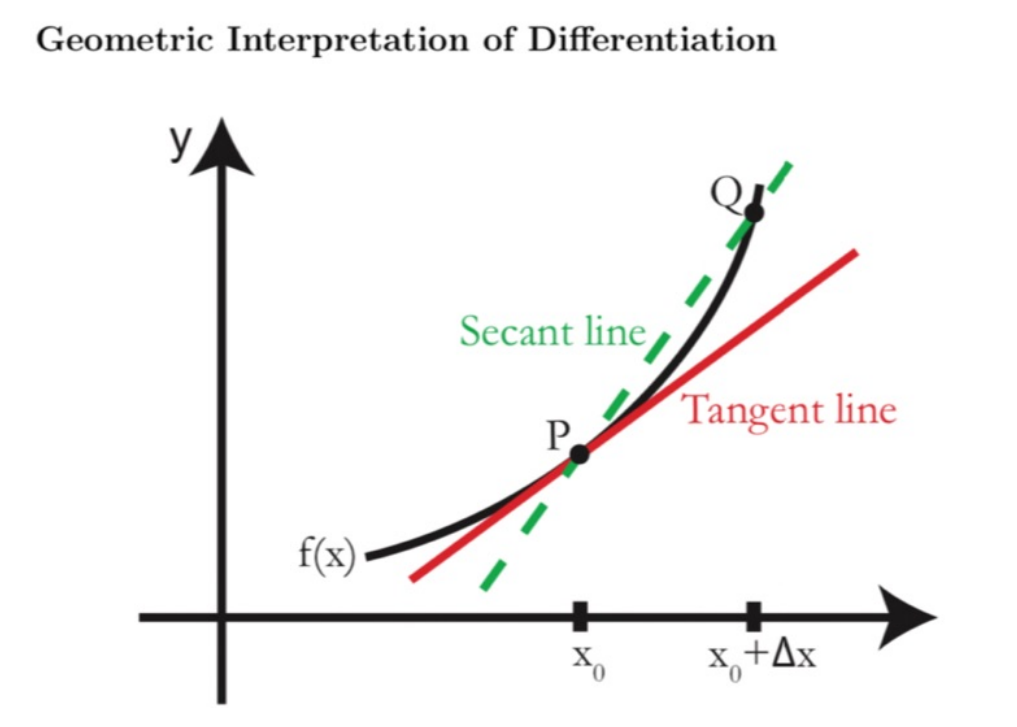
\includegraphics[width=9cm]{Capture}
\centering
\end{figure}
\noindent The derivative of $f(x)$ at $x=x_0$ is the slope of the tangent line to $f(x)$ at the
point $(x_0,f(x_0))$. Supposing $PQ$ is a secant line of $f(x)$, the tangent line can be viewed
as the limit of secant lines $PQ$ as $Q\to P$ ($P$ is fixed while $Q$ varies).
\newpage
\noindent Now consider a closer perspective of the secant line:
\begin{figure}[h]
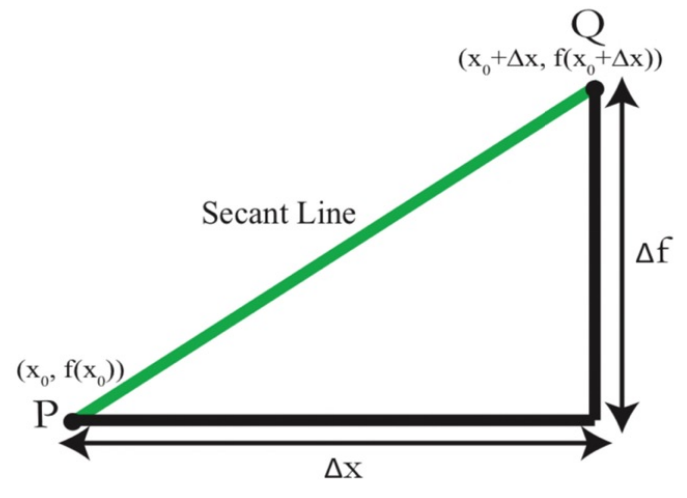
\includegraphics[width=9cm]{Capture2}
\centering
\end{figure}
Since the derivative is the slope of the tangent line at $P$, it is also the slope of the secant
line as $Q\to P$; therefore:
\begin{align*}
\underbrace{m}_{\text{derivative}}=\lim_{Q\to P}\frac{\Delta f}{\Delta x}
=\lim_{\Delta x\to 0}\frac{\Delta f}{\Delta x}
\end{align*}
Since we can further define $\Delta f=f(x_0+\Delta x)-f(x_0)$, We can now formulate the derivative as:
\begin{align*}
m=f'(x_0)=\lim_{\Delta x\to 0}\frac{\Delta f}{\Delta x}
=\underbrace{\lim_{\Delta x\to 0}\frac{f(x_0+\Delta x)-f(x_0)}{\Delta x}}
_{\text{\textbf{Difference quotient}}}
\end{align*}
A machine could use this formula together with coordinates $(x_0.f(x_0))$ to draw a tangent line.
This formula also serves as the basis for many other proofs for derivatives.
\newpage

\subsection{Derivative of $\frac{1}{x}$} %130524
As mentioned in \ref{fundamentals:differentiation:definition}, the formula for the derivative:
\begin{equation*}
f'(x)=\lim_{\Delta x\to 0}\frac{f(x_0+\Delta x)-f(x_0)}{\Delta x}
\end{equation*}
is fundamental to deriving many other functions; here we find the derivative of the function
$f(x)=\frac{1}{x}$ at point $x=x_0$. First we formulate the gradient of the secant line:
\begin{align*}
\frac{\Delta f}{\Delta x}&=\frac{f(x_0+\Delta x)-f(x_0)}{\Delta x}\\
&=\frac{\frac{1}{x_0+\Delta x}-\frac{1}{x_0}}{\Delta x}\\
&=\frac{(x_0+\Delta x)(x_0)}{(x_0+\Delta x)(x_0)}
\frac{\frac{1}{x_0+\Delta x}-\frac{1}{x_0}}{\Delta x}\\
&=\frac{x_0-(x_0+\Delta x)}{(x_0+\Delta x)(x_0)(\Delta x)}\\
&=\frac{-\Delta x}{(x_0+\Delta x)(x_0)(\Delta x)}\\
&=\frac{-1}{(x_0+\Delta x)(x_0)}
\end{align*}
Next, as $\Delta x$ tends to zero:
\begin{align*}
f'(x)=\lim_{\Delta x\to 0}\frac{\Delta f}{\Delta x}
=\lim_{\Delta x\to 0}\frac{-1}{(x_0+\Delta x)(x_0)}=\Aboxed{-\frac{1}{x_0^2}}
\end{align*}

\subsection{Notation} %130524
Note the typical notation for the derivative comes from taking the limit as $\Delta x\to 0$:
\begin{align*}
\frac{\Delta y}{\Delta x}&\to \frac{dy}{dx}&\text{(Leibniz' notation)}\\
\frac{\Delta f}{\Delta x}&\to f'(x_0)&\text{(Newton's notation)}
\end{align*}
Note that:
\begin{equation*}
\Delta y=\Delta f=f(x)-f(x_0)=f(x_0+\Delta x)-f(x_0)
\end{equation*}

\newpage
\subsection{Derivative of $x^n$ where $n=1,2,3\ldots$ (Power rule)} %130524
We plug $y=f(x)$ into the definiton of the difference quotient 
(see \ref{fundamentals:differentiation:definition}):
\begin{equation*}
\frac{\Delta y}{\Delta x}=\frac{f(x+\Delta x)-f(x)}{\Delta x}=\frac{(x+\Delta x)^n-x^n}{\Delta x}
\end{equation*}
Since $(x+\Delta x)^n$ can be written as:
\begin{equation*}
(x+\Delta x)(x+\Delta x)\ldots (x+\Delta x)\quad\text{(n times)}
\end{equation*}
It can be rewritten as:
\begin{equation*}
(x+\Delta x)^n=x^n+n(\Delta x)x^{n-1}+O(\Delta x)^2
\end{equation*}
where $O(\Delta x)^2$ represents all the terms containing  $(\Delta x)^2, (\Delta x)^3$, and so on
up till $(\Delta x)^n$. (Regarding $n(\Delta x)x^{n-1}$, consider that there were $n$ different
$\Delta x$'s that one could choose to multiply by, so one gets this result $n$ different ways.)\\
\vspace{2mm}\\
Returning to the difference quotient:
\begin{equation*}
\frac{\Delta y}{\Delta x}=\frac{(x+\Delta x)^n-x^n}{\Delta x}
=\frac{(x^n+n(\Delta x)x^{n-1}+O(\Delta x)^2)-x^n}{\Delta x}
=nx^{n-1}+O(\Delta x)
\end{equation*}
(Where $O(\Delta x)$ represents all the terms containing  $(\Delta x), (\Delta x)^2
\ldots(\Delta x)^n$.)\\
\vspace{2mm}\\
Taking the limit as $\Delta x\to 0$:
\begin{equation*}
\lim_{\Delta x\to 0}\frac{\Delta y}{\Delta x}=nx^{n-1}
\end{equation*}
and therefore,
\begin{equation*}
\underbrace{\frac{d}{dx}x^n=nx^{n-1}}_{\text{\textbf{power rule}}}
\end{equation*}
\newpage

\subsection{Derivative of a Sum}%150524
Here we prove, where $u$ and $v$ are differentiable functions of $x$:
\begin{equation*}
(u+v)'(x)=u'(x)+v'(x)
\end{equation*}
Note that $(u+v)(x)=u(x)+v(x)$\\
\vspace{2mm}\\
\textbf{Proof:} using the difference quotient:
\begin{align*}
(u+v)'(x)&=\lim_{\Delta x\to 0}\frac{(u+v)(x+\Delta x)-(u+v)(x)}{\Delta x}\\
&=\lim_{\Delta x\to 0}\frac{u(x+\Delta x)+v(x+\Delta x)-u(x)-v(x)}{\Delta x}\\
&=\lim_{\Delta x\to 0}\left\{\frac{u(x+\Delta x)-u(x)}{\Delta x}+
\frac{v(x+\Delta x)-v(x)}{\Delta x}\right\}\\
\end{align*}
Because $u$ and $v$ are differentiable (and therefore continuous), the limit of the sum is the
sum of the limits. Therefore:
\begin{align*}
(u+v)'(x)&=\lim_{\Delta x\to 0}\frac{u(x+\Delta x)-u(x)}{\Delta x}
+\lim_{\Delta x\to 0}\frac{v(x+\Delta x)-v(x)}{\Delta x}\\
&=u'(x)+v'(x)
\end{align*}
\newpage

\subsection{Proof of limit for $\lim_{x\to 0}\frac{\sin x}{x}$} %150524
In order to compute specific formulas for the derivatives of $\sin x$ and $\cos x$, we run into 
the the limit $\lim_{\Delta x\to 0}\frac{\sin\Delta x}{\Delta x}$. Here we show that
\begin{equation*}
\lim_{x\to 0}\frac{\sin x}{x}=1
\end{equation*}
Using $\theta$ as our parameter, consider:
\begin{figure}[h]
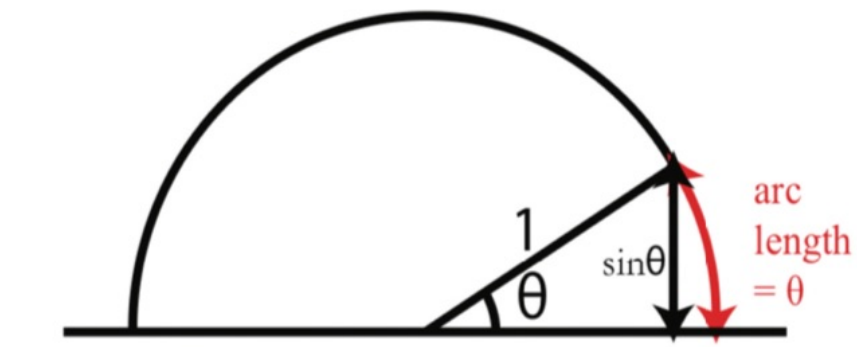
\includegraphics[width=9cm]{Capture7}
\centering
\text{\textbf{Figure:} Radius 1, arc of angle $\theta$}
\end{figure}\\
Notice that our function of interest $\frac{\sin\theta}{\theta}$ is the ratio of the edge length
to the arc length.
(Note the highlighted arc length is only equal to $\theta$ when $\theta$ is measured in
\textbf{radians})\\
\vspace{2mm}\\
Now consider what happens as $\theta$ becomes smaller.\\ When $\theta=\frac{\pi}{2}$ rad,
$\sin\theta=1$ and $\frac{\sin\theta}{\theta}=\frac{2}{\pi}\approx\frac{2}{3}$.\\
When $\theta=\frac{\pi}{4}$ rad,
$\sin\theta=\frac{\sqrt{2}}{2}$ and $\frac{\sin\theta}{\theta}=\frac{2\sqrt{2}}{\pi}
\approx\frac{9}{10}$.\\
\begin{figure}[h]
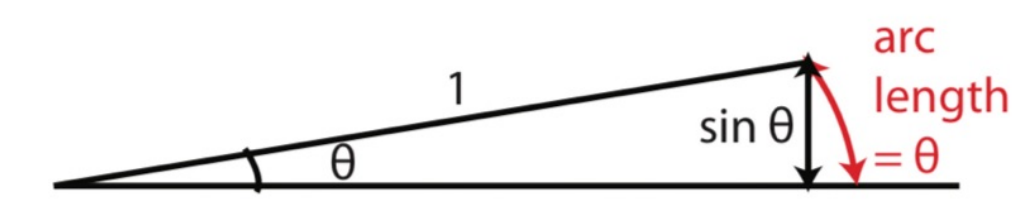
\includegraphics[width=9cm]{Capture8}
\centering
\text{\textbf{Figure:} What happens as $\theta$ becomes very small?}
\end{figure}\\
As $\theta$ shrinks, the length of the segment $\sin\theta$ gets closer to the arc length $\theta$
; thus we conclude:
\begin{align*}
\lim_{\theta\to 0}\frac{\sin\theta}{\theta}&=1\quad\text{and}\\
\lim_{x\to 0}\frac{\sin x}{x}&=1
\end{align*}
\newpage

\subsection{Proof of limit for $\lim_{x\to 0}\frac{1-\cos x}{x}$}%150524
In order to compute specific formulas for the derivatives of $\sin x$ and $\cos x$, we run into 
the the limit $\lim_{\Delta x\to 0}\frac{\cos\Delta x-1}{\Delta x}$. Here we show that
\begin{equation*}
\lim_{x\to 0}\frac{1-\cos x}{x}=\lim_{x\to 0}\frac{\cos x-1}{x}=0
\end{equation*}
Using $\theta$ as our parameter, consider:
\begin{figure}[h]
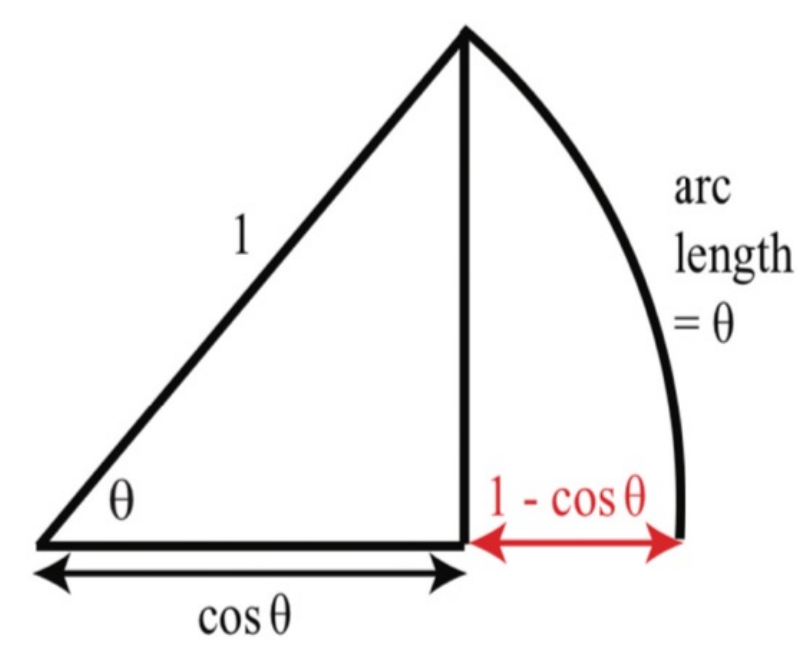
\includegraphics[width=9cm]{Capture9}
\centering
\text{\textbf{Figure:} Radius 1, arc of angle $\theta$}
\end{figure}\\ 
Notice that as $\theta\to 0$, the horizontal gap $1-\cos\theta$ gets much smaller compared to
the length of the arc (This can be confirmed with a calculator or any graphing tool):
\begin{figure}[h]
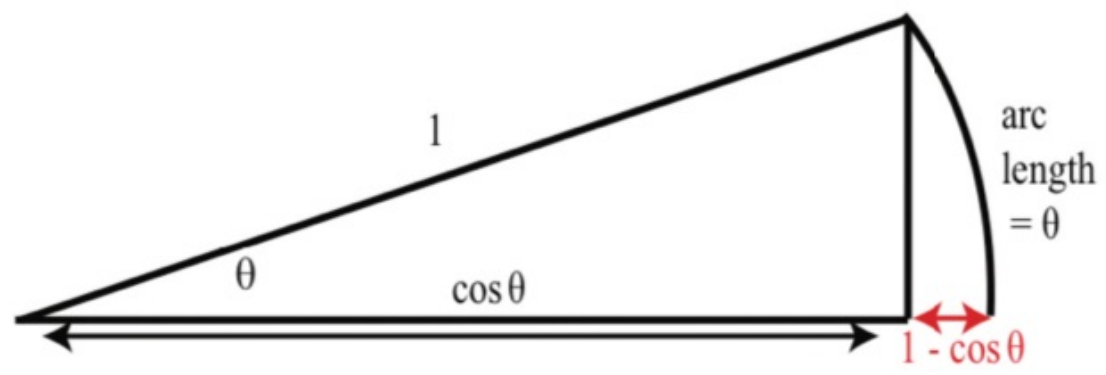
\includegraphics[width=9cm]{Capture10}
\centering
\text{\textbf{Figure:} as $\theta$ becomes very small}
\end{figure}\\ 
(next page)
\newpage    
\noindent Since $|1-\cos\theta|$ becomes increasingly smaller than 
$\theta$ as $\theta$ decreases, we can conclude:
\begin{align*}
\lim_{x\to 0}\frac{1-\cos\theta}{\theta}&=\lim_{x\to 0}\frac{\cos\theta-1}{\theta}
=0\quad\text{and}\\
\lim_{x\to 0}\frac{1-\cos x}{x}&=\lim_{x\to 0}\frac{\cos x-1}{x}=0
\end{align*}

\newpage
\subsection{Derivative of $\sin x$, Algebraic proof; Angle formulas} %150524
Here we compute a specific formula for the derivative of $\sin x$. We begin with the
definition of the derivative/difference quotient:
\begin{equation*}
\frac{d}{dx}\sin x=\lim_{\Delta x\to 0}\frac{\sin(x+\Delta x)-\sin x}{\Delta x}
\end{equation*}
using the angle formula (proof below):
\begin{equation*}
\sin(a+b)=\sin(a)\cos(b)+\sin(b)\cos(a)
\end{equation*}
we get:
\begin{align*}
\frac{d}{dx}\sin x&=\lim_{\Delta x\to 0}\frac{(\sin x\cos\Delta x+\sin\Delta x\cos x)-\sin x}
{\Delta x}\\
&=\lim_{\Delta x\to 0}\left[\frac{\sin x(\cos\Delta x-1)}{\Delta x}+
\frac{\sin\Delta x\cos x}{\Delta x}\right]\\
&=\lim_{\Delta x\to 0}\sin x\left(\frac{\cos\Delta x-1}{\Delta x}\right)+
\lim_{\Delta x\to 0}\cos x\left(\frac{\sin\Delta x}{\Delta x}\right)\\
&=\sin x\lim_{\Delta x\to 0}\left(\frac{\cos\Delta x-1}{\Delta x}\right)
+\cos x\lim_{\Delta x\to 0}\left(\frac{\sin\Delta x}{\Delta x}\right)
\end{align*}
Using the fact that
\begin{align*}
&\lim_{\Delta x\to 0}\frac{\cos\Delta x-1}{\Delta x}=0\quad\text{and}\\
&\lim_{\Delta x\to 0}\frac{\sin\Delta x}{\Delta x}=1
\end{align*}
We conclude:
\begin{align*}
\frac{d}{dx}\sin x&=\sin x\lim_{\Delta x\to 0}\left(\frac{\cos\Delta x-1}{\Delta x}\right)
+\cos x\lim_{\Delta x\to 0}\left(\frac{\sin\Delta x}{\Delta x}\right)\\
&=\cos x
\end{align*}
(Proof of angle formula on next page)
\newpage
Proof of:
\begin{align*}
&\sin(\alpha+\beta)=\sin\alpha\cos\beta+\sin\beta\cos\alpha\quad\text{and}\\
&\cos(\alpha+\beta)=\cos\alpha\cos\beta-\sin\alpha\sin\beta
\end{align*}
\begin{figure}[h]
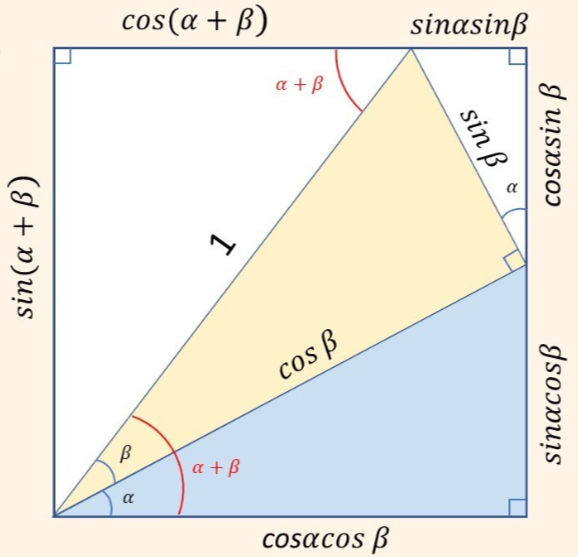
\includegraphics[width=9cm]{Capture6}
\centering
\end{figure}
\newpage

\subsection{Derivative of $\cos x$, Algebraic proof} %150524
Here we compute a specific formula for the derivative of $\cos x$. We begin with the
definition of the derivative/difference quotient:
\begin{equation*}
\frac{d}{dx}\cos x=\lim_{\Delta x\to 0}\frac{\cos(x+\Delta x)-\cos x}{\Delta x}
\end{equation*}
using the angle formula
\begin{equation*}
\cos(a+b)=\cos a\cos b-\sin a\sin b
\end{equation*}
we get:
\begin{align*}
\frac{d}{dx}\cos x&=\lim_{\Delta x\to 0}\frac{\cos(x+\Delta x)-\cos x}{\Delta x}\\
&=\lim_{\Delta x\to 0}\frac{(\cos x\cos\Delta x-\sin x\sin\Delta x)-\cos x}{\Delta x}\\
&=\lim_{\Delta x\to 0}\left[\cos x\frac{\cos\Delta x-1}{\Delta x}
-\sin x\frac{\sin\Delta x}{\Delta x}\right]\\
&=\cos x\lim_{\Delta x\to 0}\frac{\cos\Delta x-1}{\Delta x}
-\sin x\lim_{\Delta x\to 0}\frac{\sin\Delta x}{\Delta x}
\end{align*}
Using the fact that
\begin{align*}
&\lim_{\Delta x\to 0}\frac{\cos\Delta x-1}{\Delta x}=0\quad\text{and}\\
&\lim_{\Delta x\to 0}\frac{\sin\Delta x}{\Delta x}=1
\end{align*}
We conclude:
\begin{align*}
\frac{d}{dx}\cos x&=\cos x\lim_{\Delta x\to 0}\frac{\cos\Delta x-1}{\Delta x}
-\sin x\lim_{\Delta x\to 0}\frac{\sin\Delta x}{\Delta x}\\
&=-\sin x
\end{align*}
\newpage

\subsection{Derivative of $\sin x$, Geometric proof} %150524
This appendix also contains an algebraic proof for the derivative of $\sin x$; however while that
proof was valid, it did not make use of the definition of the sine function. Here we prove that
the derivative of $\sin\theta$ is $\cos\theta$ directly from the definition of the sine function 
as the ratio $\frac{|\text{opposite}|}{|\text{hypotenuse}|}$ of the a right triangle.
Consider a circle:
\begin{figure}[h]
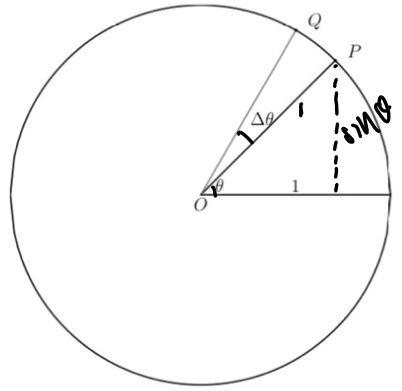
\includegraphics[width=9cm]{Capture11}
\centering\\
\text{\textbf{Figure:} point $P=\sin\theta$}
\end{figure}\\
Notice that $\sin\theta$ is the vertical distance between $P$ and the $x$ axis,
we increment $\theta$ slightly by the addition of $\Delta\theta$.
Notice now that point $Q$ is the point on the unit 
circle at angle $\theta+\Delta\theta$, and that the $y$-coordinate of $Q$ is
$\sin(\theta+\Delta\theta)$. To find the rate of change of $\sin\theta$ with respect to $\theta$
we just need to find the rate of change of $y=\sin\theta$.\\
(next page)
\newpage
\noindent Now consider a close-up view of segment $PQ$:
\begin{figure}[h]
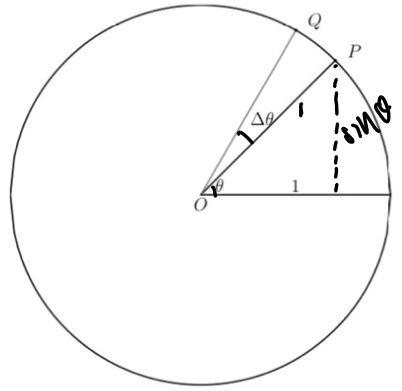
\includegraphics[width=5cm]{Capture11}
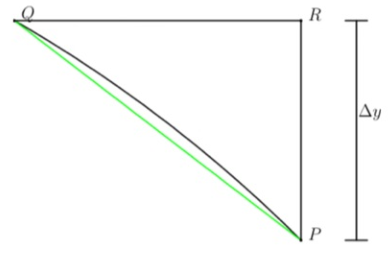
\includegraphics[width=5cm]{Capture12}
\centering\\
\text{\textbf{Figure:} When $\Delta\theta$ is small, \textbf{segment} $PQ\approx$ 
\textbf{arc} $PQ$}
\end{figure}\\
Notice that $\Delta y=|PR|$ and \textbf{segment} $PQ$ is a straight line that approximates to 
\textbf{arc} $PQ$ as $\Delta\theta$ becomes smaller. Also note that since the circle is of 
radius 1, arc $PQ=\Delta\theta$ and segment
$PQ\approx\Delta\theta$ (as $\Delta\theta$ decreases).\\
\vspace{2mm}\\
Since $\Delta\theta$ is small, segment $PQ$ is (nearly) tangent to the circle, and angle
$\angle OPQ$ is (nearly) a right angle. We can say therefore that $\angle RPQ$ and $\theta$ are
(nearly) congruent angles.\\
\vspace{2mm}\\
The arc $PQ=\Delta\theta$ approximates to $|PQ|$(hypotenuse), and $\angle RPQ$ 
approximates to $\theta$ (As $\Delta\theta$ becomes small). Now consider that
$\cos\theta\approx\cos(\angle RPQ)$ and therefore
\begin{equation*}
\cos\theta\approx\frac{|PR|}{\Delta\theta}=\frac{\Delta y}{\Delta\theta}
=\frac{\sin(\theta+\Delta\theta)-\sin\theta}{\Delta\theta}\quad
\text{(As $\Delta\theta$ becomes small)}
\end{equation*}
As $\Delta\theta\to0$ \textbf{arc} $PQ$ approximates \textbf{segment} $PQ$ more closely and 
$\angle OPQ$ approximates a right angle more closely. This means that
$\frac{\sin(\theta+\Delta\theta)-\sin\theta}{\Delta\theta}$ more closely approximates 
$\cos\theta$. We can therefore conclude that:
\begin{equation*}
\underbrace{\lim_{\Delta\theta\to0}\frac{\sin(\theta+\Delta\theta)-\sin\theta}
{\Delta\theta}}_{\frac{d}{dx}\sin\theta}=\cos\theta
\end{equation*}
\newpage

\subsection{Product rule} %160522
Here we prove the product rule, the derivative of the product of two functions:
\begin{equation*}
(uv)'=u'v+uv'
\end{equation*}
We start with the definition of the derivative:
\begin{align*}
\frac{d}{dx}(uv)&=\lim_{\Delta x\to0}\frac{(uv)(x+\Delta x)-(uv)(x)}{\Delta x}\\
&=\lim_{\Delta x\to0}\frac{u(x+\Delta x)v(x+\Delta x)-u(x)v(x)}{\Delta x}\\
=\lim_{\Delta x\to0}&\frac{u(x+\Delta x)v(x+\Delta x)-u(x)v(x)
+u(x+\Delta x)v(x)-u(x+\Delta x)v(x)}{\Delta x}\\
=\lim_{\Delta x\to0}&\frac{u(x+\Delta x)(v(x+\Delta x)-v(x))
+v(x)(u(x+\Delta x)-u(x))}{\Delta x}\\
=\lim_{\Delta x\to0}&\left[u(x+\Delta x)\frac{v(x+\Delta x)-v(x)}{\Delta x}\right]
+v(x)\left[\lim_{\Delta x\to0}\frac{u(x+\Delta x)-u(x))}{\Delta x}\right]\\
&=u(x)v'(x)+v(x)u'(x)\\
&=u'(x)v(x)+u(x)v'(x)
\end{align*}
Note we used the fact that:
\begin{equation*}
\lim_{\Delta x\to0}u(x+\Delta x)=u(x)
\end{equation*}
This works because we assume $u$ is differentiable and continuous.
\newpage

\subsection{Quotient rule} %170524
Here we derive a specific function for differentiating quotients (fractions), the quotient rule:
\begin{equation*}
\left(\frac{u}{v}\right)'=\frac{u'v-uv'}{v^2}
\end{equation*}
(Note that this can simply be seen as an extension of taking the derivative of
$(uv^{-1})$, where the product rule can also be used.)\\
\vspace{2mm}\\
We start with the definition of the derivative:
\begin{equation*}
\left(\frac{u}{v}\right)'=\lim_{\Delta x\to0}\frac{\frac{u(x+\Delta x)}{v(x+\Delta x)}
-\frac{u(x)}{v(x)}}{\Delta x}
\end{equation*}
First we simplify the numerator using:
\begin{align*}
u(x+\Delta x)-u(x)&=\Delta u\quad\text{(not $u(\Delta x)$)}\\
u(x+\Delta x)&=u(x)+\Delta u 
\end{align*}
where
\begin{align*}
\frac{u(x+\Delta x)}{v(x+\Delta x)}-\frac{u(x)}{v(x)}&=\frac{u+\Delta u}{v+\Delta v}
-\frac{u}{v}\\
&=\frac{v(u+\Delta u)-u(v+\Delta v)}{v(v+\Delta v)}\\
&=\frac{(\Delta u)v-u(\Delta v)}{v(v+\Delta v)}
\end{align*}
Now back to the derivative:
\begin{align*}
\lim_{\Delta x\to0}\frac{\frac{u(x+\Delta x)}{v(x+\Delta x)}-\frac{u(x)}{v(x)}}{\Delta x}
&=\lim_{\Delta x\to0}\frac{\frac{(\Delta u)v-u(\Delta v)}{v(v+\Delta v)}}{\Delta x}\\
&=\lim_{\Delta x\to0}\frac{1}{\Delta x}\frac{(\Delta u)v-u(\Delta v)}{v(v+\Delta v)}\\
&=\lim_{\Delta x\to0}\frac{\left(\frac{\Delta u}{\Delta x}\right)v
-u\left(\frac{\Delta v}{\Delta x}\right)}{v(v+\Delta v)}\\
=&\frac{u'v-uv'}{v^2}
\end{align*}
\newpage

\subsection{Quotient rule derived from Product and Chain rule} %170524
As mentioned earlier, the Quotient rule is simply an extension of the product rule and the
chain rule:
\begin{align*}
\left(\frac{f(x)}{g(x)}\right)'=(f(x)(g(x))^{-1})'
\end{align*}
First we find the derivative of $(g(x))^{-1}$ using the chain rule:
\begin{align*}
\frac{d}{dx}(g(x))^{-1}&=\frac{d}{dg}(g(x))^{-1}\cdot\frac{d}{dx}g(x)\\
&=-(g(x))^{-2}\cdot g'(x)
\end{align*}
Therefore:
\begin{align*}
\left(\frac{f(x)}{g(x)}\right)'&=(f(x)(g(x))^{-1})'\\
&=f'(x)(g(x))^{-1}+f(x)((g(x))^{-1})'\\
&=f'(x)(g(x))^{-1}+f(x)(-(g(x))^{-2}g'(x))\\
&=\left[f'(x)g(x)-f(x)g'(x)\right](g(x))^{-2}\\
&=\underbrace{\frac{f'(x)g(x)-f(x)g'(x)}{(g(x))^2}}_{\text{product rule}}
\end{align*}
\newpage

\subsection{Chain rule} %170524
The composition or ''chain'' rule tells us how to find the derivative of a composition of
functions like $f(g(x))$ (note this is \textbf{not} the same as $fg(x)$).
\begin{figure}[h]
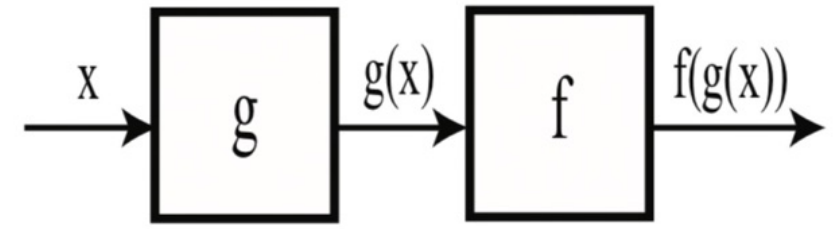
\includegraphics[width=10cm]{Capture13}
\centering\\
\text{\textbf{Figure:} Composition of functions: $(f\circ g)(x)=f(g(x))$}
\end{figure}\\
The chain rule can be viewed as using an intermediate variable to find a derivative. Consider
trying to find $\frac{dy}{dt}$:
\begin{align*}
\frac{\Delta y}{\Delta t}&=\frac{\Delta y}{\Delta x}\cdot\frac{\Delta x}{\Delta t}\\
\lim_{\Delta t\to0}\frac{\Delta y}{\Delta t}&=
\underbrace{\frac{dy}{dt}=\frac{dy}{dx}\cdot\frac{dx}{dt}}_{\text{\textbf{chain rule}}}
\end{align*}
The chain rule can also be written as
\begin{equation*}
\frac{d}{dx}(f\circ g)(x)=\frac{d}{dx}f(g(x))=\underbrace{f'(g(x))\cdot g'(x)}
_{\frac{dy}{dx}\cdot\frac{dx}{dt}}
\end{equation*}

\subsection{Chain rule example: $\frac{d}{dt}\sin^nt$} %170524
\textbf{Example:} Consider $y=\sin^{n}t$ (in the form of $y(t)$), where we want to
find $\frac{dy}{dt}$; we can introduce a function $x$ where $x=\sin t$, and now 
$y=x^{n}$ (notice it is now in the form $y(x(t)$). Now applying the chain rule:
\begin{align*}
\frac{dy}{dt}=\frac{d}{dt}\sin^{n}t&=\frac{dy}{dx}\cdot\frac{dx}{dt}\\
&=\frac{dy}{dx}x^{n}\cdot\frac{d}{dt}\sin t\\
&=nx^{n-1}\cdot\cos t\\
&=n\sin^{n-1} t\cdot\cos t
\end{align*}
\newpage

\subsection{Chain rule example: $\frac{d}{dt}\sin(nt)$} %170524
\textbf{Example:} Consider $y=\sin(nt)$ (in the form of $y(t)$),
where we want to find $\frac{dy}{dt}$; we can introduce a function $x$ where $x=nt$, 
and now $y=\sin x$ (notice it is now in the form $y(x(t)$). Now applying the chain rule:
\begin{align*}
\frac{dy}{dt}=\frac{d}{dt}\sin nt&=\frac{dy}{dx}\cdot\frac{dx}{dt}\\
&=\frac{dy}{dx}\sin x\cdot\frac{d}{dt}nt\\
&=\cos x\cdot n\\
&=n\cos(nt)
\end{align*}
\newpage

\subsection{Derivative of $y=x^a$, where a is rational: Rational exponent rule
(via implicit differentiation)} %180524
Here we prove the rational exponent rule, where
\begin{equation*}
\frac{d}{dx}x^a=ax^{a-1}
\end{equation*}
Where $a$ is a rational number (i.e $\frac{m}{n}$)\\
\vspace{2mm}\\
Consider $y=x^{\frac{m}{n}}$, where $m$ and $n$ are integers; we want to compute $\frac{dy}{dx}$.
Unlike most proofs, starting with the definition of derivative does not work here (since we 
get stuck on $(x+\Delta x)^{\frac{m}{n}}$). We get around this by:
\begin{align*}
y&=x^{\frac{m}{n}}\\
y^n&=x^{\frac{m}{n}\cdot n}\\
y^n&=x^m
\end{align*} 
Now we perform \textbf{implicit differentiation}, where we take the derivative of a function
that cannot be explicitly expressed as $f(x)$, in this case $y^n$:
\begin{align*}
y^n&=x^m\\
\frac{d}{dx}y^n&=\frac{d}{dx}x^m
\end{align*}
using the chain rule to simplify $\frac{d}{dx}y^n$:
\begin{align*}
\frac{d}{dx}y^n&=\frac{d}{dy}y^n\cdot\frac{dy}{dx}\\
&=ny^{n-1}\frac{dy}{dx}
\end{align*}
we now have:
\begin{align*}
\frac{d}{dx}y^n&=\frac{d}{dx}x^m\\
ny^{n-1}\frac{dy}{dx}&=mx^{m-1}
\end{align*}
(next page)
\newpage
\noindent Now we can rearrange:
\begin{align*}
ny^{n-1}\frac{dy}{dx}&=mx^{m-1}\\
\frac{dy}{dx}&=\frac{mx^{m-1}}{ny^{n-1}}
\end{align*}
Finally we can replace $y$ with $x^{\frac{m}{n}}$:
\begin{align*}
\frac{dy}{dx}&=\frac{mx^{m-1}}{ny^{n-1}}\\
&=\frac{m}{n}\left(\frac{x^{m-1}}{x^{\frac{m}{n}\cdot(n-1)}}\right)\\
&=\frac{m}{n}x^{(m-1)-\frac{m(n-1)}{n}}\\
&=\frac{m}{n}x^{\frac{n(m-1)}{n}-\frac{m(n-1)}{n}}\\
&=\frac{m}{n}x^{\frac{m-n}{n}}\\
&=\frac{m}{n}x^{(\frac{m}{n}-1)}
\end{align*}
For any rational number $a$, the derivative of $x^a$ is $ax^{a-1}$.
\newpage

\subsection{Derivative of the inverse of a function} %180524
Consider $f(x)=\sqrt{x}$ plotted against its inverse function:
\begin{figure}[h]
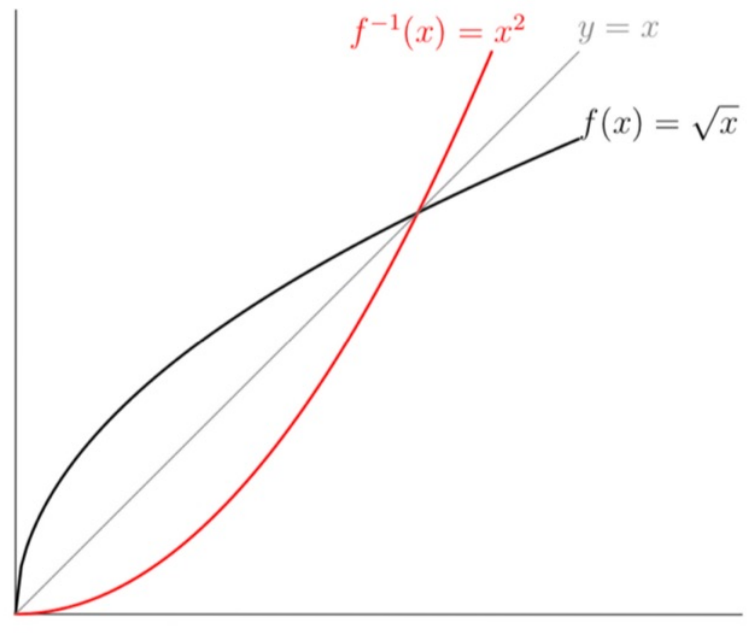
\includegraphics[width=7cm]{Capture14}
\centering
\text{\textbf{Figure:} $f^{-1}(x)$ is a reflection of $f(x)$ across the line $y=x$}
\end{figure}\\
Since an inverse function $f^{-1}$ can generally be found by exchanging the $x-$ and 
$y-$coordinates of $f$ (a reflection across $y=x$), one might posit that if $\frac{dy}{dx}$ is
the slope of a line tangent to $f$, then
\begin{equation*}
\frac{dx}{dy}=\frac{1}{(\frac{dy}{dx})}
\end{equation*}
would be the slope of a line tangent to $f^{-1}$. Here we prove this through
implicit differentiation; consider:
\begin{align*}
y&=f(x)\\
f^{-1}(y)&=x\\
\frac{d}{dx}(f^{-1}(y))&=\frac{d}{dx}x=1
\end{align*}
by the chain rule:
\begin{align*}
&\frac{d}{dy}(f^{-1}(y))\frac{dy}{dx}=1\\
&\frac{d}{dy}(f^{-1}(y))=\frac{1}{\frac{dy}{dx}}
\end{align*}
\newpage

\subsection{Derivative of $\tan(x)$ and $\arctan(x)$/$\tan^{-1}(x)$} %180524
\textbf{Derivative of $\tan(x)$:}\\
First we prove the derivative of $\tan(x)$ using the product rule:
\begin{align*}
\tan(x)&=\frac{\sin(x)}{\cos(x)}\\
\frac{d}{dx}\tan(x)&=\frac{d}{dx}\frac{\sin(x)}{\cos(x)}\\
\end{align*}
Now by product rule:
\begin{align*}
\frac{d}{dx}\frac{\sin(x)}{\cos(x)}&=\frac{\cos(x)\cdot\cos(x)
-\sin(x)\cdot(-\sin(x))}{(\cos(x))^{2}}\\
&=\frac{\sin^2(x)+\cos^2(x)}{\cos^2(x)}\\
&=\frac{1}{\cos^2(x)}=\sec^2(x)
\end{align*}
\vspace{2mm}\\
\textbf{Derivative of $\arctan(x)$/$\tan^{-1}(x)$}:
Here we use implicit differentiation to find the derivative of $y=\tan^{-1}(x)=\arctan(x)$:
\begin{align*}
y&=\tan^{-1}(x)\\
\tan(y)&=x\\
\frac{d}{dx}\tan(y)&=\frac{d}{dx}x\\
\frac{d}{dy}\tan(y)\cdot\frac{dy}{dx}&=1\quad\text{(Chain rule)}\\
\frac{1}{\cos^2(y)}\cdot\frac{dy}{dx}&=1\\
\frac{dy}{dx}&=\cos^2(y)
\end{align*}
Now we can substitute in $y=\tan^{-1}(x)$ to get
\begin{equation*}
\frac{dy}{dx}=\cos^2(\tan^{-1}(x))
\end{equation*}
Although this result is valid, it can still be simplified greatly.\\
(next page)
\newpage
\noindent Our earlier result was:
\begin{align*}
\frac{dy}{dx}&=\cos^2(y)\\
\frac{dy}{dx}&=\cos^2(\tan^{-1}(x))
\end{align*}
We can use geometry to simplify this result; consider:
\begin{figure}[h]
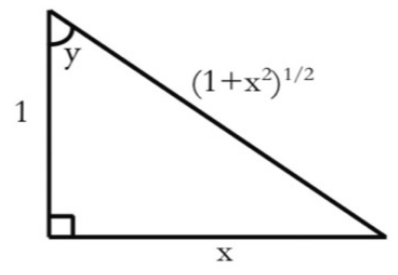
\includegraphics[width=6cm]{Capture15}\\
\centering
\text{\textbf{Figure:} Triangle where $\tan(y)=x$}
\end{figure}\\
Using the Pythagorean theorem we know that the hypotenuse of this theoretical triangle is
\begin{equation*}
h=\sqrt{1+x^2}
\end{equation*}
so now we can compute
\begin{align*}
\cos(y)&=\frac{1}{\sqrt{1+x^2}}\\
\cos^2(y)&=\frac{1}{1+x^2}\\
\end{align*}
Therefore,
\begin{equation*}
\frac{d}{dx}\tan^{-1}(x)=\frac{d}{dx}\arctan(x)=\frac{dy}{dx}=\cos^2(y)=\frac{1}{1+x^2}
\end{equation*}
\newpage

\subsection{Derivative of $\arcsin(x)$/$\sin^{-1}(x)$} %190524
\label{fundamentals:differentiation:arcsin}
We can solve for the derivative of $y=\arcsin(x)=\sin^{-1}(x)$ by implicit differentiation:
\begin{align*}
y&=\sin^{-1}(x)\\
\sin(y)&=x\\
\frac{d}{dx}\sin(y)&=\frac{d}{dx}x\\
\frac{d}{dy}\sin(y)\cdot\frac{dy}{dx}&=1\\
(\cos(y))\cdot\frac{dy}{dx}&=1\\
\frac{dy}{dx}&=\frac{1}{\cos(y)}\\
\end{align*}
Since
\begin{align*}
&\sin^2(y)+\cos^2(y)=1\\
&\cos(y)=\sqrt{1-\sin^2(y)}
\end{align*}
(Notice that we made a choice between a positive and negative square root when solving for 
$\cos(y)$. We chose the positive square root as $\sin^{-1}(x)$ is usually defined to have outputs
between $-\pi/2$ and $\pi/2$, a range in which the cosine function is always positive.)\\
\vspace{2mm}\\
We can now simplify the derivative:
\begin{align*}
\frac{dy}{dx}&=\frac{1}{\cos(y)}\\
&=\frac{1}{\sqrt{1-\sin^2(y)}}\\
&=\frac{1}{\sqrt{1-x^2}}
\end{align*}
\newpage

\subsection{Intuition and definition of $e$\\(Derivative of $a^x$ part 1)} %190524
\label{introduction:differentiation:$e$}
Here we attempt to provide an introduction and a sense of intuition to Euler's number $e$. 
This is done by attempting to find the derivative of $a^x$, where $e$ is a natural result
that falls out of the math during the derivation.\\
\vspace{1mm}\\
We begin with the goal of calculating the derivative $\frac{d}{dx}a^x$. We start with the
definition of the derivative:
\begin{align*}
\frac{d}{dx}a^x&=\lim_{\Delta x\to0}\frac{a^{x+\Delta x}-a^x}{\Delta x}\\
&=\lim_{\Delta x\to0}\frac{a^xa^{\Delta x}-a^x}{\Delta x}\\
&=\lim_{\Delta x\to0}a^x\frac{a^{\Delta x}-1}{\Delta x}\\
&=a^x\lim_{\Delta x\to0}\frac{a^{\Delta x}-1}{\Delta x}
\end{align*}
We can see that $\frac{d}{dx}a^x$ is $a^x$ multiplied by some value that we don't yet know. 
We denote that value by $M(a)$:
\begin{equation*}
M(a)=\lim_{\Delta x\to0}\frac{a^{\Delta x}-1}{\Delta x}
\end{equation*}
So
\begin{equation*}
\frac{d}{dx}a^x=M(a)a^x
\end{equation*}
Notice that when we plug $x=0$ into the definition of the derivative $\frac{d}{dx}a^x$:
\begin{align*}
\left.\frac{d}{dx}a^x\right|_{x=0}&=
\lim_{\Delta x\to0}\left.\frac{a^{x+\Delta x}-a^x}{\Delta x}\right|_{x=0}\\
&=\lim_{\Delta x\to0}\frac{a^{0+\Delta x}-a^0}{\Delta x}\\
&=\lim_{\Delta x\to0}\frac{a^{\Delta x}-1}{\Delta x}=M(a)
\end{align*}
(we could also observe that $\left.\frac{d}{dx}a^x\right|_{x=0}=M(a)a^0=M(a)$)\\
\vspace{1mm}\\
\textbf{Notice that $M(a)$ is the value of the derivative of $a^x$ when $x=0$.}\\
(next page)
\newpage
\noindent\textbf{On the necessity for $e$:} The result
\begin{equation*}
\left.\frac{d}{dx}a^x\right|_{x=0}=M(a)=\lim_{\Delta x\to0}\frac{a^{\Delta x}-1}{\Delta x}
\end{equation*}
indicates that $M(a)$ can be thought of as the gradient of $a^x$ at $x=0$, meaning we only
need to know the value of the gradient at $x=0$ to know the gradient at any point on the curve
(note that the shape of the curve depends on the value of $a$, resulting in different
tangent lines and different $M(a)$): 
\begin{figure}[h]
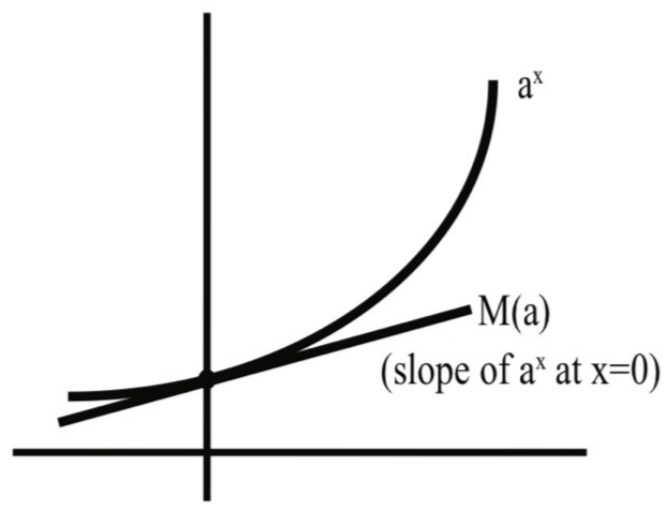
\includegraphics[width=8cm]{Capture16}\\
\centering
\text{\textbf{Figure:} Geometric definition of $M(x)$}
\end{figure}\\
However, one runs into difficulty when attempting to exactly identify $M(a)$. This issue is
circumvented by the introduction of $e$.\\
\vspace{1mm}\\
\textbf{Definition of $e$:}\\
We need to know what $M(a)$ is to find the derivative of $a^x$. It turns out the easiest way to 
understand $M(a)$ is to give up trying to calculate it and to \textit{define} a number 
$e$ as the number where $M(e)=1$. This would lead to the result
\begin{equation*}
\frac{d}{dx}e^x=e^x
\end{equation*}
The gradient of the tangent line to $y=e^x$ at $x=0$ is 1. This can be confirmed:
\begin{equation*}
\left.\frac{d}{dx}e^x\right|_{x=0}=e^0=1
\end{equation*}
(next page)
\newpage
\noindent\textbf{On the existence and identity of $e$:}\\
We define $e$ to be the number where:
\begin{equation*}
\frac{d}{dx}e^x=e^x,\quad M(e)=1
\end{equation*}
Now we elaborate on why $e$ exists. We know that the $M(a)$ (gradient of $a^x$ at $x=0$) 
increases as $a$ increases. Consider:
\begin{figure}[h]
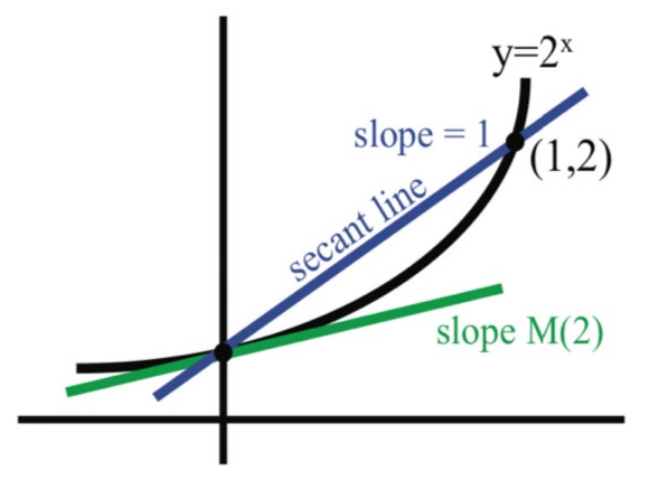
\includegraphics[width=4.8cm]{Capture17}
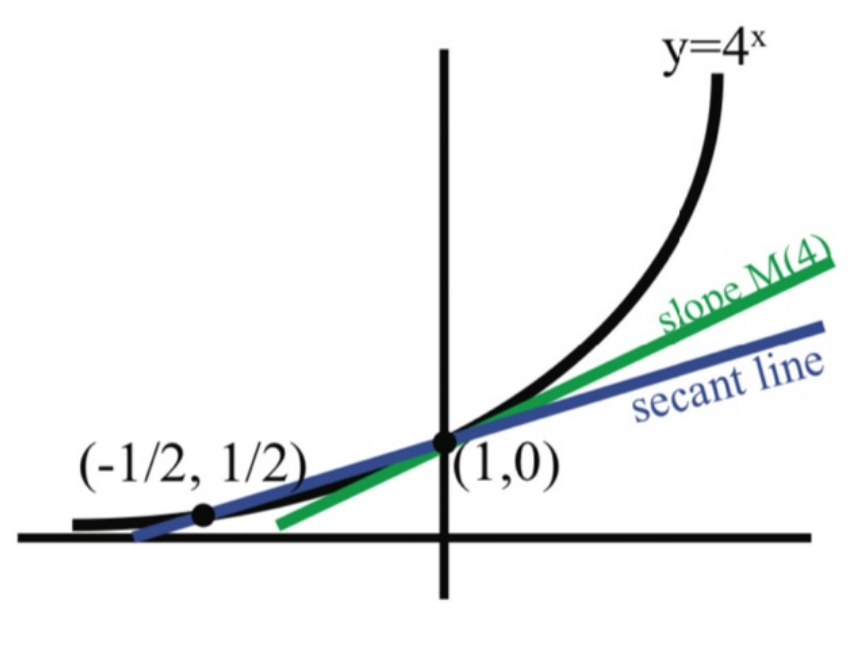
\includegraphics[width=5cm]{Capture18}
\centering
\text{\textbf{Left:} $M(2)$ compared with secant line of gradient 1}\\
\text{\textbf{Right:} $M(4)$ compared with secant line of gradient 1}
\end{figure}\\
The figures plot $y=2^x$ (left) and $y=4^x$ (right) against $y=x+1$ (line of gradient 1 
passing through (1,0)). Notice that $M(2)<1$ while $M(4)>1$. Using this we can conclude
that $e$ exists, and that $2<e<4$.\\
\vspace{1mm}\\
In conclusion, we define $e$ as the unique number where:
\begin{equation*}
M(e)=1
\end{equation*}
or
\begin{equation*}
\lim_{h\to0}\frac{e^h-1}{h}=1
\end{equation*}
or
\begin{equation*}
\frac{d}{dx}e^x=1\quad\text{at $x=0$}
\end{equation*}

\subsection{Differentiating $e^{f(x)}$} %210524
\begin{align*}
\frac{d}{dx}e^{f(x)}&=\frac{d}{df}e^{f(x)}\cdot\frac{df}{dx}\quad\text{(chain rule)}\\
&=e^{f(x)}\cdot\frac{df}{dx}\\
&=f'(x)e^{f(x)}
\end{align*}
\newpage

\subsection{Natural Logarithm and its derivative} %200524
\textbf{Intuition and definition:}\\
Recall that:
\begin{equation*}
M(a)=\lim_{\Delta x\to0}\frac{a^{\Delta x}-1}{\Delta x}
\end{equation*}
Is the value for the derivative $\frac{d}{dx}a^x=M(a)a^x$, and is equivalent to the value of the
derivative of $a^x$ at $x=0$ ($\left.\frac{d}{dx}a^x\right|_{x=0}$ gives $M(a)$). Also recall
how this naturally leads to $e$ ($M(e)=0$ so $\frac{d}{dx}e^x=e^x$) 
(see \ref{introduction:differentiation:$e$}).\\
\vspace{1mm}\\
Here we introduce and derive the natural logarithm. The natural log function $\ln(x)$ is the 
inverse of the function $e^x$; it is defined as follows:
\begin{equation*}
\text{If}\quad y=e^x,\quad\text{then}\quad\ln(y)=x
\end{equation*}
or
\begin{equation*}
\text{If}\quad w=\ln(x),\quad\text{then}\quad x=e^w
\end{equation*}
\vspace{1mm}\\
\textbf{Properties}: The natural log has additive properties:
\begin{equation*}
\ln(x_1x_2)=\ln(x_1)+\ln(x_2)
\end{equation*}
This can be proved with simple concepts, consider:
\begin{equation*}
x_1=a\quad\text{and}\quad x_2=b
\end{equation*}
so, since $e^{\ln(x)}$ is equivalent to $f(f^{-1}(x))=x$: 
\begin{equation*}
x_1=e^{\ln(a)}\quad\text{and}\quad x_2=e^{\ln(b)}
\end{equation*}
therefore
\begin{align*}
\ln(x_1x_2)&=\ln(e^{\ln(a)}e^{\ln(b)})\\
&=\ln(e^{(\ln(a)+\ln(b))})\\
&=(\ln(a)+\ln(b))=\ln(x_1)+\ln(x_2)
\end{align*}
Other properties also include:
\begin{equation*}
\ln(1)=0\quad(\ln(e^0)=0)
\end{equation*}
\begin{equation*}
\ln(e)=1\quad(\ln(e^1)=e)
\end{equation*}
Also note that the nature of $\ln(x)$ as the inverse of $e^x$ means that it lies entirely to the
right of the $y$-axis, and has a gradient of 1 at $x=0$ ($\left.\frac{dx}{dy}e^x\right|_{x=0}$).
Next we find the derivative of $\ln(x)$.\\
(next page)
\newpage
\noindent\textbf{Derivative of natural log:} We use implicit differentiation:
\begin{align*}
y&=\ln(x)\\
e^y&=x\\
\frac{d}{dx}e^y&=\frac{d}{dx}x\\
\frac{d}{dy}e^y\cdot\frac{dy}{dx}&=1\quad\text{(chain rule)}\\
e^y\cdot\frac{dy}{dx}&=1\\
\frac{dy}{dx}&=\frac{1}{e^y}\\
\end{align*}
Since $y=\ln(x)$ and $e^y=x$:
\begin{align*}
\frac{dy}{dx}=\frac{d}{dx}\ln(x)&=\frac{1}{e^y}=\frac{1}{x}\\
\frac{d}{dx}\ln(x)&=\frac{1}{x}
\end{align*}
And for function $f(x)$, differentiating $\ln(f(x))$:
\begin{align*}
\frac{d}{dx}\ln(f(x))&=\frac{d}{df}\ln(f(x))\cdot\frac{df}{dx}\quad\text{(chain rule)}\\
&=\frac{1}{f(x)}\cdot f'(x)\\
&=\frac{f'(x)}{f(x)}
\end{align*}

\subsection{Proof of $\ln(a^x)=x\ln(a)$} %210524
Here we prove:
\begin{equation*}
\ln(a^x)=x\ln(a)
\end{equation*}
Since $e^{\ln(x)}=x$,
\begin{align*}
\ln(a^x)&=\ln((e^{\ln(a)})^x)\\
&=\ln(e^{x\ln(a)})\\
&=x\ln(a)
\end{align*}
\newpage

\subsection{Derivative of $a^x$ part 2} %210524-220524
Here we outline the the derivative of $a^x$, this can be done through different methods:\\
\textbf{Method 1: Conversion to base $e$}\\
Since (by chain rule) $\frac{d}{dx}e^{f(x)}=f'(x)e^{f(x)}$, we convert the base to $e$:
\begin{align*}
\frac{d}{dx}a^x&=\frac{d}{dx}(e^{\ln(a)})^x\\
&=\frac{d}{dx}e^{\ln(a)x}\\
&=\frac{d}{dx}(\ln(a)x)\cdot e^{\ln(a)x}\\
&=\ln(a)a^x
\end{align*}
Recall that $\frac{d}{dx}a^x=M(a)\cdot a^x$. We can now define $M(a)$:  
\begin{equation*}
M(a)=\ln(a)
\end{equation*}
\textbf{Method 2: Logarithmic}\\
We can use $\frac{d}{dx}\ln(f(x))=\frac{f'(x)}{f(x)}$ to avoid changing bases and differentiate implicitly:
\begin{align*}
y&=a^x\\
\ln(y)&=\ln(a^x)\\
\frac{d}{dx}\ln(y)&=\frac{d}{dx}(x\ln(a))\\
\frac{d}{dy}\ln(y)\frac{dy}{dx}&=\ln(a)\quad\text{(chain rule)}\\
\frac{1}{y}\frac{dy}{dx}&=\ln(a)\\
\frac{dy}{dx}&=\ln(a)y\\
&=\ln(a)a^x
\end{align*}
Note therefore that both methods yield the same solution:
\begin{equation*}
\frac{d}{dx}a^x=\ln(a)a^x
\end{equation*}
\newpage

\subsection{$\frac{d}{dx}x^r=rx^{r-1}$ for any \textit{real} $r$\\ (another power rule proof)}
Earlier in this appendix are sections detailing proofs of the power rule regarding the derivative
of $x^r$ for integer and rational values of $r$. Here we show two proofs that the power rule
\begin{equation*}
\frac{d}{dx}x^r=rx^{r-1}
\end{equation*}
applies for any \textit{real} value of $r$.\\
\vspace{1mm}\\
\textbf{Method 1: Base $e$}\\
Since $x=e^{\ln(x)}$,
\begin{align*}
x^r&=(e^{\ln(x)})^r\\
\frac{d}{dx}x^r&=\frac{d}{dx}(e^{r\ln(x)})\\
&=\frac{d}{dx}(r\ln(x))e^{r\ln(x)}\\
&=\frac{r}{x}e^{r\ln(x)}\\
&=\frac{r}{x}x^r\\
&=rx^{r-1}
\end{align*}
\textbf{Method 2: Logarithmic}\\
We start with the fact that, defining $f(x)=x^r$
\begin{align*}
(\ln(f))'&=\frac{f'}{f}\\
f'&=f(\ln(f))'
\end{align*}
Now we find $(\ln(f))'$:
\begin{align*}
(\ln(f))'&=(\ln(x^r))'\\
&=(r\ln(x))'\\
&=\frac{r}{x}
\end{align*}
Therefore,
\begin{equation*}
f'=f(\ln(f))'=(x^r)\frac{r}{x}=rx^{r-1}
\end{equation*}
\newpage

\subsection{On the value of $e$ (Moving exponent)} %230524
Here we present a method for computing the value of $e$. This comes from attempting to
find the value of the limit
\begin{equation*}
\lim_{n\to\infty}\left(1+\frac{1}{n}\right)^n
\end{equation*}
Note that this limit contains a moving exponent $n$. To begin evaluating the limit we
first apply a logarithm to turn the exponent into a multiple.
\begin{equation*}
\ln\left(1+\frac{1}{n}\right)^n=n\ln\left(1+\frac{1}{n}\right)
\end{equation*}
Now consider the idea that
\begin{equation*}
\lim_{n\to\infty}\frac{1}{n}=\lim_{\Delta x\to0}\Delta x
\end{equation*}
We apply that idea here, changing the limit to substitute $\frac{1}{n}$ for $\Delta x$:
\begin{align*}
\lim_{n\to\infty}\left[n\ln\left(1+\frac{1}{n}\right)\right]&=
\lim_{\Delta x\to0}\left[\frac{1}{\Delta x}\ln\left(1+\Delta x\right)\right]\\
&=\lim_{\Delta x\to0}\left[\frac{\ln(1+\Delta x)-\ln(1)}{\Delta x}\right]\quad
\text{(since $\ln(1)=\ln(e^0)=0$)}\\
&=\left.\frac{d}{dx}\ln(x)\right|_{x=1}
=\left.\frac{1}{x}\right|_{x=1}=1
\end{align*}
Now we return to the original problem:
\begin{align*}
\lim_{n\to\infty}\left(1+\frac{1}{n}\right)^n
&=\lim_{n\to\infty}\left(e^{\ln(1+\frac{1}{n})}\right)^n\\
&=\lim_{n\to\infty}e^{n\ln(1+\frac{1}{n})}\\
&=e^{\lim_{n\to\infty}\left[n\ln(1+\frac{1}{n})\right]}\\
&=e^1=e
\end{align*}
Therefore, since $e$ happens to be the result where
\begin{equation*}
\lim_{n\to\infty}\left(1+\frac{1}{n}\right)^n=e
\end{equation*}
We can use this to compute a value of $e$. For instance
\begin{equation*}
\left(1+\frac{1}{10000}\right)^{10000}\approx 2.7182
\end{equation*}
\newpage

\subsection{Derivatives of Hyperbolic Sine and Cosine}
Hyperbolic sine:
\begin{equation*}
\sinh(x)=\frac{e^x-e^{-x}}{2}
\end{equation*}
Hyperbolic cosine:
\begin{equation*}
\cosh(x)=\frac{e^x+e^{-x}}{2}
\end{equation*}
Intuition for these hyperbolic functions comes from Euler's notation,
see [TBD].\\
\vspace{1mm}\\
The derivative of $\sinh(x)$ is $\cosh(x)$ and vice versa:
\begin{align*}
\frac{d}{dx}\sinh(x)=\frac{d}{dx}\left(\frac{e^x-e^{-x}}{2}\right)
&=\left(\frac{e^x+e^{-x})}{2}\right)=\cosh(x)\\
\text{likewise,}\quad\frac{d}{dx}\cosh(x)&=\sinh(x)
\end{align*}
Also note an important identity:
\begin{equation*}
\cosh^2(x)-\sinh^2(x)=1
\end{equation*}
Proof:
\begin{align*}
\cosh^2(x)-\sinh^2(x)&=\left(\frac{e^x+e^{-x}}{2}\right)^2
-\left(\frac{e^x-e^{-x}}{2}\right)^2\\
&=\frac{1}{4}(e^{2x}+2e^xe^{-x}+e^{-2x})
-\frac{1}{4}(e^{2x}-2e^xe^{-x}+e^{-2x})\\
&=1
\end{align*}
\textbf{Some intuition:}\\
Letting $u=\cosh(x)$ and $v=\sinh(x)$, then
\begin{equation*}
u^2-v^2=1
\end{equation*}
Which is the equation of a hyperbola
\newpage

%%%%%%%%%%%%%%%%%%%%%%%%%%%%%%%%%%%%%
%% applications of differentiation %%
%%%%%%%%%%%%%%%%%%%%%%%%%%%%%%%%%%%%%

\section{Applications of differentiation}

\subsection{Intuition for Linear approximation} %230524
\textbf{Graphical intuition}\\
Consider a curve $f(x)$; now consider an $x$-coordinate $x_0$. One can intuit 
that the curve is approximately the same as its tangent line 
$y=f(x_0)+f'(x_0)(x-x_0)$:
\begin{figure}[h]
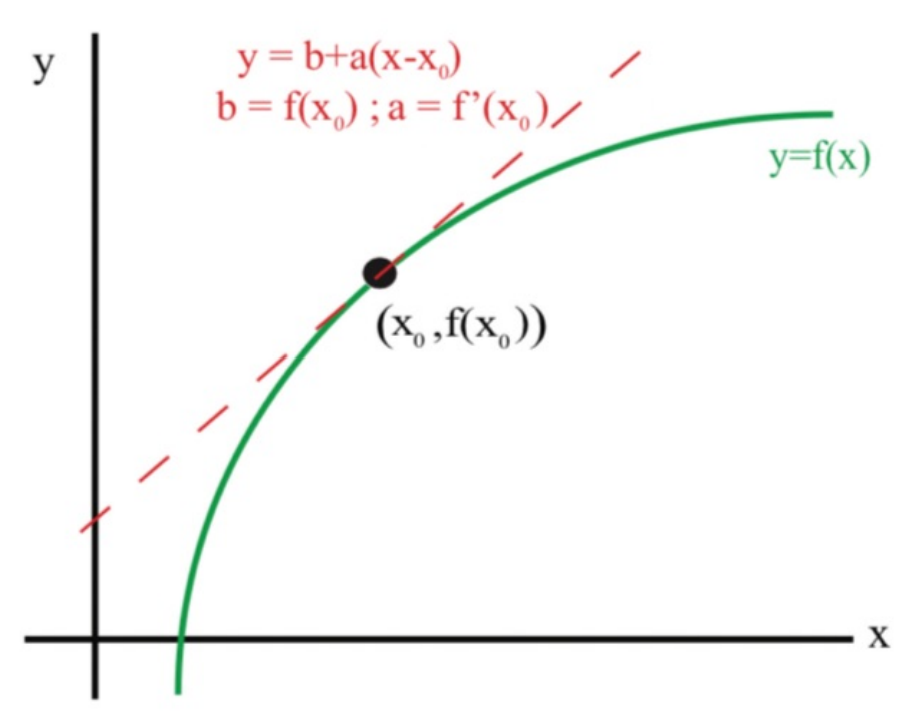
\includegraphics[width=9cm]{Capture19}\\
\centering
\text{\textbf{Figure:} approximation grows less accurate moving away from $x_0$}
\end{figure}\\
The tangent line approximates $f(x)$ near the tangent point $x_0$. However, moving
away from $x_0$, the approximation
\begin{equation*}
f(x)\approx f(x_0)+f'(x_0)(x-x_0)
\end{equation*}
grows less accurate.\\
(next page)
\newpage
\noindent\textbf{Intuition from the derivative}\\
Another way to understand the formula for linear approximation involves
the definition of the derivative:
\begin{equation*}
f'(x_0)=\lim_{\Delta x\to0}\frac{\Delta f}{\Delta x}
\end{equation*}
This can be interpreted to mean:
\begin{equation*}
\frac{\Delta f}{\Delta x}\approx f'(x_0)\quad\text{as $\Delta x\to0$}
\end{equation*}
Note that $\Delta x$ refers to $x-x_0$, allowing us to rewrite:
\begin{align*}
\frac{f(x)-f(x_0)}{x-x_0}&\approx f'(x)\\
f(x)-f(x_0)&\approx f'(x_0)(x-x_0)\\
f(x)&\approx f(x_0)+f'(x_0)(x-x_0)
\end{align*}
\newpage

\subsection{Linear approximations near 0 for\\ Sine, Cosine, and Exponential functions} %230524
Here we describe the linear approximation of several common functions at 0. 
To simplify things we use base point $x_0=0$ and assume that $x\approx 0$; this gives us 
a simplified general formula:
\begin{align*}
f(x)\approx f(&x_0)+f'(x_0)(x-x_0)\\
&\text{becomes}\\
f(x)\approx &f(0)+f'(0)(x)
\end{align*}
Note therefore that these approximations won't work when $x$ is not near 0.\\
We summarise the values of $f'(x),f(x),f'(0)$ and $f(0)$ as follows:
\begin{align*}
&f(x)    & &f'(x)    & &f(0) & &f'(0)\\
&\sin(x) & &\cos(x)  & &0    & &1\\
&\cos(x) & -&\sin(x) & &1    & &0\\
&e^x     & &e^x      & &1    & &1
\end{align*}
Plugging the above values into our simplified formula $
f(x)\approx f(0)+f'(0)(x)$, we get:
\begin{align*}
1.&\quad\sin(x)\approx x\quad\text{(if $x\approx 0$)}\quad\text{(see figure (a))}\\
2.&\quad\cos(x)\approx 1\quad\text{(if $x\approx 0$)}\quad\text{(see figure (b))}\\
3.&\quad e^x\approx 1+x\quad\text{(if $x\approx 0$)}
\end{align*}
\begin{figure}[h]
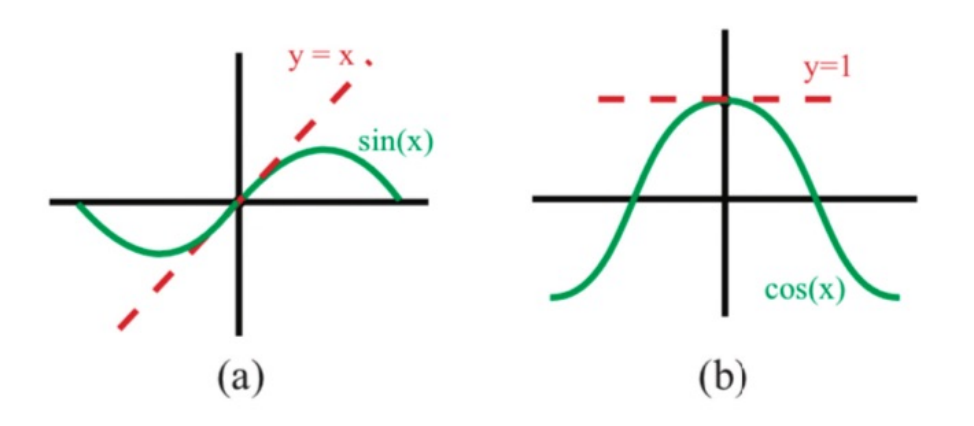
\includegraphics[width=9cm]{Capture20}
\centering
\text{\textbf{Figures:} Graphical intuition for linear approximations when $x\approx 0$}
\end{figure}
\newpage

\subsection{Linear approximations near 0 for\\$\ln(1+x)$ and $(1-x)^r$} %230524
Here we describe the linear approximation of $\ln(1+x)$ and $(1-x)^r$ at 0. 
To simplify things we use base point $x_0=0$ and assume that $x\approx 0$; this gives us 
a simplified general formula:
\begin{align*}
f(x)\approx f(&x_0)+f'(x_0)(x-x_0)\\
&\text{becomes}\\
f(x)\approx &f(0)+f'(0)(x)
\end{align*}
We summarise the values of $f'(x),f(x),f'(0)$ and $f(0)$ as follows:
\begin{align*}
&f(x)     & &f'(x)          & &f(0) & &f'(0)\\
&\ln(1+x) & &\frac{1}{1+x}  & &0    & &1\\
&(1+x)^r  & &r(1-x)^{r-1}   & &1    & &r
\end{align*}
This gives us the approximations:
\begin{align*}
1.&\quad\ln(1+x)\approx x\quad\text{(if $x\approx 0$)}\\
2.&\quad(1-x)^r\approx 1+rx\quad\text{(if $x\approx 0$)}
\end{align*}
Note that we approximate $\ln(1+x)$ because $\ln(x)\to -\infty$ as $x\to0$.
Similarly, we approximate $(1+x)^r$ because apparently for some values of $r$
$x^r$ is not well behaved when $x=0$. If we really need an approximation for $x^r$ 
we can get one via change of variables.\\
\textbf{Example of change of variables}\\
Approximating $\ln(x)$ at $x\approx 1$ via the linear approximation formula:
\begin{equation*}
f(x)\approx f(x_0)+f'(x_0)(x-x_0)
\end{equation*}
Where $x_0=1$ in this case, gives us $\ln(x)\approx x-1$. Notice that by substituing
$u\approx 1+x$ into the result it yields:
\begin{align*}
\ln(x)\approx x-1&\quad\text{for $x\approx 1$}\\
\text{becomes}\\
\underbrace{\ln(1+u)\approx u}_{\text{derived above}}&\quad\text{for $u\approx 0$}
\end{align*}
Therefore, knowing $\ln(x)\approx x-1$ for $x\approx1$, one can approximate $\ln(1+u)$ by change of variables. (vice versa works too)
\newpage

\subsection{Quadratic Approximation - Definition and Intuition} %240524
\textbf{Formula}\\
Quadratic approximation can be seen as an extension of linear approximation.
The formula for quadratic approximation is as follows:
\begin{equation*}
f(x)\approx \underbrace{f(x_0)+f'(x_0)(x-x_0)}_{\text{Linear part}}
+\underbrace{\frac{f''(x_0)}{2}(x-x_0)^2}_{\text{Quadratic part}}
\quad\text{for $(x\approx x_0)$}
\end{equation*}
\textbf{Intuition}\\
Consider attempting to approximate a function that is a parabola. Intuitively, 
if the graph of a function is a parabola, that function \textit{is a quadratic function} 
and would therefore be best approximated by an identical quadratic function. Consider:
\begin{equation*}
f(x)=a+bx+cx^2;\quad f'(x)=b+2cx;\quad f''(x)=2c
\end{equation*}
Notice that by plugging in base point $x_0$, we can find formulas for the constants of the original function:
\begin{align*}
&f(x_0)=a+bx_0+cx_0^2\quad\implies&&a=f(x_0)-bx_0-cx_0^2\\
&f'(x_0)=b+2cx_0\quad\implies&&b=f'(x_0)-2cx_0\\
&f''(x_0)=2c\quad\implies&&c=\frac{f''(x_0)}{2}
\end{align*}
Now we attempt to find $f(x)$ (assuming $x=x_0$):
\begin{align*}
f(x)&=a+bx+cx^2\\
&=f(x_0)-bx_0-cx_0^2+bx+cx^2\quad\text{(plug in $a$)}\\
&=f(x_0)+b(x-x_0)+c(x^2-x_0^2)\\
&=f(x_0)+(f'(x_0)-2cx_0)(x-x_0)+c(x^2-x_0^2)\quad\text{($b$ now)}\\
&=f(x_0)+f'(x_0)(x-x_0)-2cx_0x+2cx_0^2+c(x^2-x_0^2)\\
&=f(x_0)+f'(x_0)(x-x_0)+c(x_0^2-2x_0x+x^2)\\
&=f(x_0)+f'(x_0)(x-x_0)+\frac{f''(x_0)}{2}(x-x_0)^2\quad\text{($c$ now)}
\end{align*}
Note that quadratic approximation would therefore obviously perfectly approximate
a \textit{quadratic} function. The point of quadratic approximation is to approximate
an otherwise oddly shaped function with a simpler polynomial.\\
\vspace{1mm}\\
One can think of quadratic approximation as an attempt
to \textit{fit} a parabola to a specific point on a function. Just as linear approximation
attempts to fit a straight line to a point on a function.
\newpage
\noindent\textbf{Geometric significance}
As mentioned, the quadratic approximation gives the best-fit parabola to a function. 
Here we consider $\cos(x)$:
\begin{figure}[h]
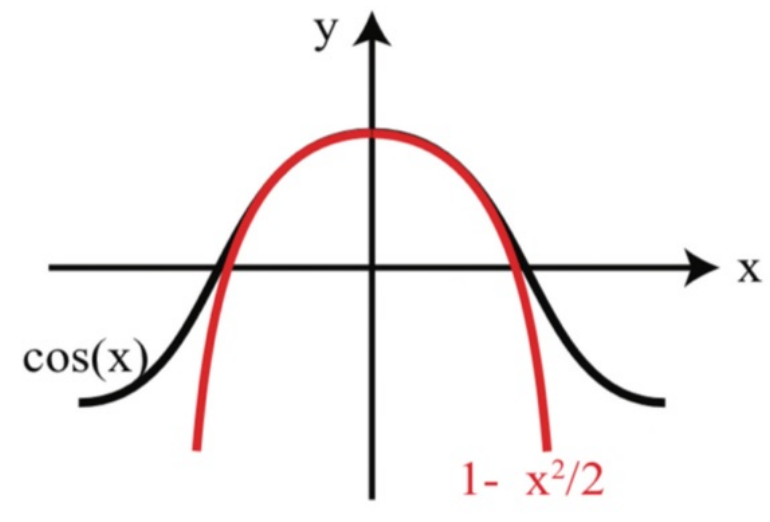
\includegraphics[width=9cm]{Capture21}\\
\centering
\text{\textbf{Figure:} Quadratic approximation to $\cos(x)$} 
\end{figure}\\
Consider a \textit{linear} approximation to $\cos(x)$ near $x_0=0$, which would 
approximate the graph by a straight horizontal line $y=1$, which obviously isn't a good approximation.\\
\vspace{1mm}\\
Now consider a similar \textit{quadratic} approximation, as illustrated. The 
geometric intuition of both linear and quadratic approximation are similar,
but quadratic approximation evidently allows for better approximation in this case.
\newpage

\subsection{Quadratic approsimations near 0} %270524
As per the formula for Quadratic Approximation:
\begin{equation*}
f(x)\approx f(x_0)+f'(x_0)(x-x_0)+\frac{f''(x_0)}{2}(x-x_0)\quad\text{where $x\approx x_0$}
\end{equation*}
Here we list the quadratic approximations at $x_0=0$ for a few common functions; 
we compute the second derivatives for the following functions, listed below:
\begin{align*}
&f(x)&&f'(x)&&f''(x)&&f(0)&&f'(0)&&f''(0)\\
&\sin(x)&&\cos(x)&-&\sin(x)&&0&&1&&0\\
&\cos(x)&-&\sin(x)&-&\cos(x)&&1&&0&-&1\\
&e^x&&e^x&&e^x&&1&&1&&1\\
\ln&(1+x)&&\frac{1}{1+x}&-&\frac{1}{(1+x)^2}&&0&&1&-&1\\
(1&+x)^r&r(1&+x)^{r-1}&r(r-1&)(1+x)^{r-1}&&1&&r&r&(r-1)
\end{align*}
Plugging in the values of $f(0),f'(0),$ and $f''(0)$:
\begin{align*}
&1.\quad\sin(x)\approx x\quad\text{(if $x\approx0$)}\\
&2.\quad\cos(x)\approx a-\frac{x^2}{2}\quad\text{(if $x\approx0$)}\\
&3.\quad e^x\approx 1+x+\frac{1}{2}x^2\quad\text{(if $x\approx0$)}\\
&4.\quad\ln(1+x)\approx x-\frac{1}{2}x^2\quad\text{(if $x\approx0$)}\\
&5.\quad(1+x)^r\approx1+rx+\frac{r(r-1)}{2}x^2\quad\text{(if $x\approx0$)}
\end{align*}
\newpage

\subsection{Degree $n$ approximation} %270524
Recall Linear and Quadratic approximation:
\begin{align*}
&\text{1. Linear:}&&f(x)\approx f(x_0)+f'(x_0)(x-x_0)\\
&\text{2. Quadratic:}&&f(x)\approx f(x_0)+f'(x_0)(x-x_0)+f''(x_0)(x-x_0)
\end{align*}
When $x\approx x_0$, $x_0$ being a predefined $x$-coordinate.\\
\vspace{1mm}\\
Linear and Quadratic approximations describe 1 and 2 degree approximations
(degree referring to the highest derivative). 
Here we define higher degree approximations, with intuition similar
to that of Linear and Quadratic approximation.\\
\vspace{1mm}\\
Here we focus on finding approximations \textit{near the value $x_0=0$}; the calculations
 for the general case are very similar. Consider a general equation for a 
higher-order polynomial (a general formula for the approximation):
\begin{equation*}
A(x)=a_0+a_1x+a_2x^2+a_3x^3+\ldots+a_{n-1}x^{n-1}a_nx^n
\end{equation*}
Consider using derivatives, and the fact that $x_0=0$ to solve for coefficients $a$:
\begin{align*}
A(x_0)=A(0)&=a_0+a_1(0)+a_2(0)+\ldots+a_n(0)\\
&=a_0+0+0+\ldots+0\quad&&a_0=A(0)\\
A'(0)&=a_1+2a_2(0)+3a_3(0)+\ldots+(n-1)a_n(0)\quad&&a_1=A'(0)\\
A^{(2)}(0)&=2a_2+6a_3(0)+\ldots+(n-1)(n-2)a_n(0)\quad&&a_2=\frac{A^{(2)}(0)}{2}\\
A^{(3)}(0)&=6a_3+\ldots+(n)(n-1)(n-1)a_n(0)\quad&&a_3=\frac{A^{(3)}(0)}{6}\\
&\quad\vdots&&\quad\vdots\\
A^{(n)}(0)&=[(n)(n-1)(n-2)\cdot\ldots\cdot(2)(1)]a_n\quad&&a_n=\frac{A^{(n)}(0)}{n!}\\
\end{align*}
So our approximation would look something like (for $x\approx x_0=0$):
\begin{equation*}
f(x)\approx A(x_0)=A(0)+A'(0)x+\frac{A^{(2)}(0)}{2}x^2+\frac{A^{(3)}(0)}{6}x^3+
\ldots+\frac{A^{(n)}(0)}{n!}x^n
\end{equation*}
(next page)
\newpage
\noindent Notice that the derivative of $a_nx^n$ is multiplied by a constant decreasing in increments of 1:
\begin{align*}
\frac{d}{dx}a_nx^n&=(n)a_nx^{n-1}\\
\frac{d^2}{dx^2}a_nx^n&=(n)(n-1)a_nx^{n-2}\\
&\vdots\\
\frac{d^n}{dx^n}a_nx^n&=(n)(n-1)\ldots(3)(2)(1)a_n\\
&=n!a_n
\end{align*}
Together, we have a general formula for each term:
\begin{equation*}
a_i\approx \frac{f^{(i)}}{i!}
\end{equation*}
With this we can conclude (when $x\approx x_0=0$):
\begin{equation*}
f(x)\approx f(0)+f'(0)x+\frac{f^{(2)}(0)}{2}x^2+\ldots
+\frac{f^{(n-1)}(0)}{(n-1)!}x^{n-1}
+\frac{f^{(n)}(0)}{n!}x^n
\end{equation*}
\newpage

\subsection{Mean Value Theorem (MVT)} %290524
Here we introduce the Mean Value Theorem (MVT);
\begin{align*}
\frac{f(b)-f(a)}{b-a}=f'(c)\quad\text{(for some $c,a<c<b$)}
\end{align*}
Provided that $f$ is \textbf{differentiable} on $a<x<b$,
and \textbf{continuous} on $a\leq x\leq b$.\\
\vspace{1mm}\\
\textbf{Geometric inutition of MVT}: Consider
a graph of $f(x)$:
\begin{figure}[h]
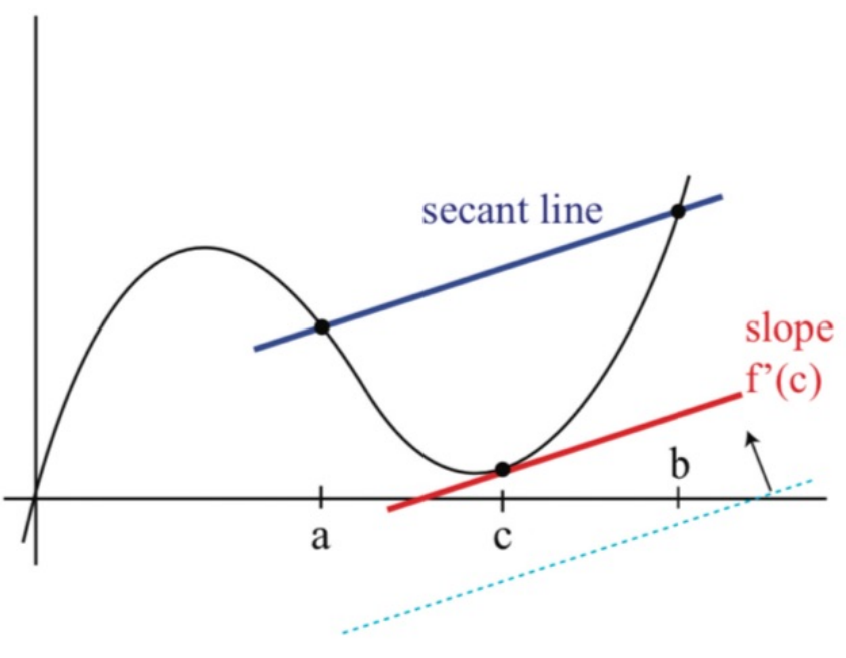
\includegraphics[width=9cm]{Capture22}\\
\centering
\text{\textbf{Figure:} A point $c$ exists where the $m_{\text{tangent}}
=m_{\text{secant}}$}
\end{figure}\\
The MVT essentially states that there is some point $c$ between $a$ and $b$ 
where the gradient of the secant line joining points $(a,f(a))$ and $(b,f(b))$ 
is equal to that of the slope of the tangent at that point 
(only if the graph is continuous and differentiable between points $a$ and $b$).\\
\vspace{1mm}\\
Geometrically this can be seen by shifting a line parallel to the secant line
vertically and noticing that it eventually touches a point between $a$ and $b$.\\
(next page)
\newpage
\noindent\textbf{MVT only works if a function is continuous and differentiable:}\\
Note that a discontinuity in the function (not continuous) or in the gradient 
of the function (not differentiable) would prevent the MVT from holding. Consider graphing $y=|x|$:\\
\begin{figure}[h]
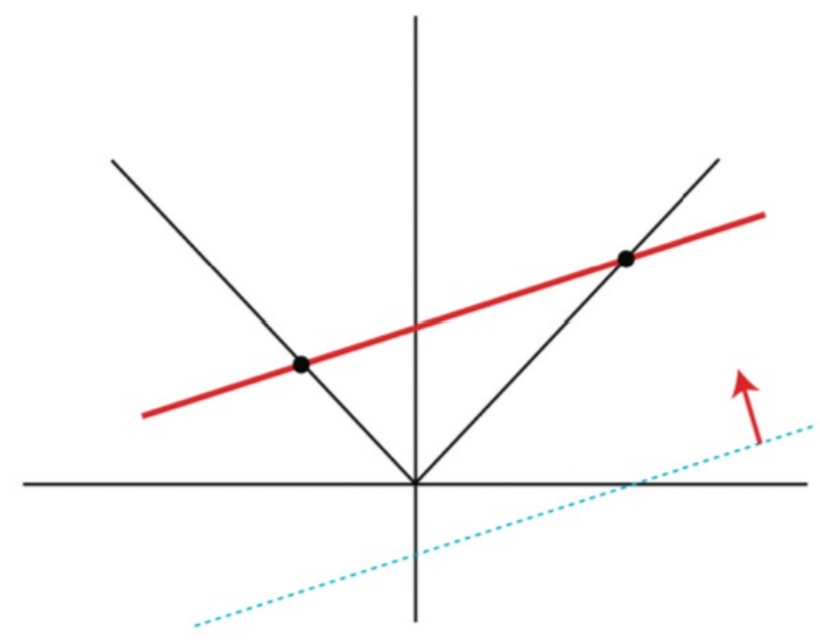
\includegraphics[width=9cm]{Capture23}\\
\centering
\text{\textbf{Figure:} $y=|x|$ is not differentiable between $a$ and $b$, MVT doesn't hold}
\end{figure}\\
Inuitively, there isn't a gradual change in gradient, meaning
that the 'range' of $f'(x)$ between $a$ and $b$ doesn't include all values
between $f'(a)$ and $f'(b)$.
\newpage

\subsection{Taylor's theorem from MVT} %300524
Here we use the Mean Value Theorem (MVT) to derive Taylor's theorem. First recall
the MVT, which states that given a continuous function $f$ on a closed interval $[a,b]$
which is differentiable on $(a,b)$, there is a number $c$ in $(a,b)$ such that 
\begin{equation*}
f'(c)=\frac{f(b)-f(a)}{b-a}
\end{equation*}
Rearranging terms, we can make this equation look similar to a that of a linear approximation
for $f(b)$ using $a$ as a base point. 
\begin{align*}
\text{from MVT:}\quad f(b)&=f(a)+f'(c)(b-a)\\
\text{linear approximation:}\quad f(b)&\approx f(a)+f'(a)(b-a)
\end{align*}
Notice that the only difference between a linear approximation is that the term $f'(a)$  
has been \textit{replaced} by $f'(c)$ for some point $c$ in order to achieve an \textbf{exact}
equality. However remember that the MVT only gives the existence of such a point $c$, 
and not a method to find $c$.\\
\vspace{1mm}\\
We interpret this as meaning that the difference between $f(b)$ and $f(a)$ is given by 
an expression resembling the \textit{next} term in the Taylor polynomial.
Here $f(a)$ is a ''0-th degree'' Taylor polynomial. A $n$-th order Taylor polynomial $P(x)$ for $f(x)$ 
with base point $x=a$ has the form:
\begin{equation*}
P(x)=f(a)+f'(a)(x-a)+\frac{f''(a)}{2}(x-a)^2+\ldots
+\frac{f^{(n)}(a)}{n!}(x-a)^n
\end{equation*}
Taylor's theorem for a first-degree Taylor polynomial is similarly:
\begin{equation*}
f(b)=\underbrace{[f(a)+f'(a)(b-a)]}_{\text{1st degree taylor polynomial}}
+\frac{f''(c)}{2}(b-a)^2
\end{equation*}
Generalising to an $n$-th degree Taylor polynomial:
\begin{align*}
&\text{\textbf{$n$-th degree approximation:}}\\
f(b)\approx&P(b)=f(a)+f'(a)(b-a)+\frac{f''(a)}{2}(b-a)^2
+\ldots+\frac{f^{(n)}(a)}{n!}(b-a)^n\\
&\text{\textbf{Using Taylor's theorem:}}\\
&f(b)=f(a)+f'(a)(b-a)+\frac{f''(a)}{2}(b-a)^2
+\ldots\\
&\quad\quad\ldots+\frac{f^{(n)}(a)}{n!}(b-a)^n+
\frac{f^{(n+1)}(a)}{(n+1)!}(b-a)^{n+1}
\end{align*}
Taylor's theorem, therefore, is the idea that given $n$-th degree Taylor polynomial:
\begin{equation*}
f(b)-P(b)=\frac{f^{(n+1)}(a)}{(n+1)!}(b-a)^{n+1}
\end{equation*}
\newpage

\subsection{Difference between linear approximation and MVT} %310524
Here we elaborate on the differences between the Mean Value Theorem (MVT) and linear approximation for the sake of intuition.\\
\vspace{1mm}\\
A linear approximation can be expressed as (for some base point $a$):
\begin{align*}
f(x)&\approx f(a)+f'(a)(x-a)\\
f(x)-f(a)&\approx f'(a)\Delta x\\
\frac{\Delta f}{\Delta x}&\approx f'(a)
\end{align*}
The MVT can be expressed similarly:
\begin{align*}
\frac{f(b)-f(a)}{b-a}&=f'(c)\quad\text{for some $c$ where $a<c<b$}\\
f(b)&=f(a)+f'(c)(b-a)\\
\frac{f(b)-f(a)}{b-a}&=f'(c)
\end{align*}
The MVT tells us that $\frac{\Delta f}{\Delta x}$ is exactly equal to $f'(c)$ for some $c$ between $a$ and $b$. 
This means that the 'average change' on the interval $[a,b]$ is between the
 minimum and maximum values of $f'(x)$ (This works because $f$ is continuous and
differentiable on the interval):
\begin{equation*}
\min_{a\leq x\leq b}\leq \frac{f(b)-f(a)}{b-a}=f'(c)\leq \max_{a\leq x\leq b}
\end{equation*}
Illustrated:
\begin{figure}[h]
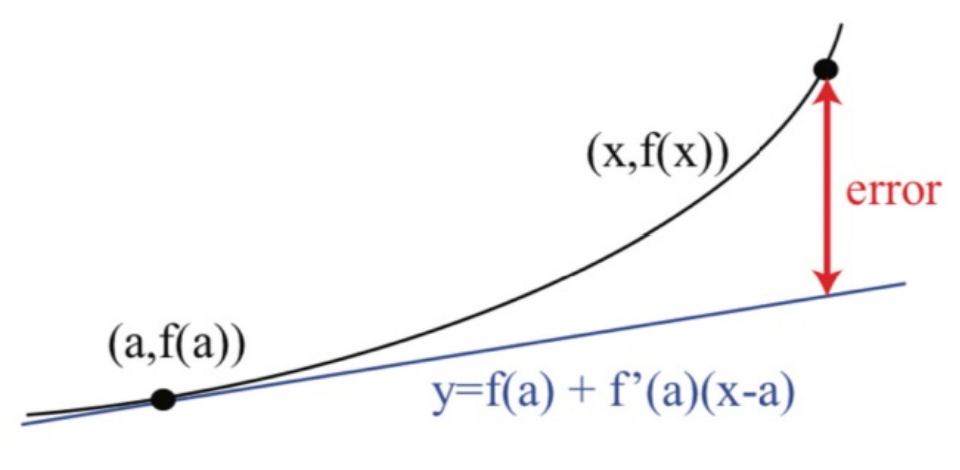
\includegraphics[width=9cm]{Capture24}\\
\centering
\text{\textbf{Figure:}  MVT vs Linear approximation}
\end{figure}\\
The MVT tells us that the slope of the secant line from $(a,f(a))$ to $(x,f(x))$ is 
between the minimum and maximum values of $f'(x)$ on the interval.
Linear approximation assumes that $f'(a)$ remains relatively constant, at least
until $(x f(x))$. Together this assures us that since Linear approximation projects
in a reasonable direction, it gives a reasonable approximation.
\newpage

\subsection{Differentials} %310524
Here we define the notation of a differential. Given a function 
$y=f(x)$, the \textit{differential} of $y$ is
\begin{equation*}
dy=f'(x)dx
\end{equation*}
Because $y=f(x)$ this can also be called the differential of $f$. 
Both $dy$ and $f'(x)dx$ are differentials. The common notation $\frac{dy}{dx}=f'(x)$ can
be thought of as the quotient of differentials.
\newpage

%%%%%%%%%%%%%%%%%
%% integration %%
%%%%%%%%%%%%%%%%%

\section{Integration}
\subsection{Antiderivatives/Indefinite Integrals} %310524
Here we introduce the notion of the antiderivative; we say 
that $G(x)=\int g(x)dx$ is the \textit{antiderivative} of $g$. Other ways of saying this are:
\begin{equation*}
G'(x)=g(x)\quad\text{or,}\quad dG=g(x)dx
\end{equation*}
Note that the definition includes a differential $dx$.
The antiderivative
\begin{equation*}
G(x)=\int g(x)dx
\end{equation*}
is also known as the \textit{indefinite integral} of $g$.\\
\vspace{1mm}\\
\textbf{Example:} $\sin x$\\
The integral/antiderivative of $g(x)=\sin x$ is the function whose derivative
is $\sin x$. Since the derivative of $-\cos x$ is $\sin x$, it is an antiderivative, $G(x)$ of $\sin x$:
\begin{align*}
G(x)&=-\cos x,\quad\text{then}\\
G'(x)&=\sin(x)=g(x)
\end{align*}
On the other hand any $G(x)=-\cos x+c$ for any constant $c$ would be valid
since the derivative of a constant is 0. Therefore we write:
\begin{equation*}
\int\sin x\,dx=-\cos x+c
\end{equation*}
This is called the \textit{indefinite integral} of $\sin x$ because $c$ can be any
constant - an indefinite value.
\newpage

\subsection{Antiderivative of $x^a$} %310524
Here we describe the antiderivative of $x^a$, which intuitively would be
\begin{align*}
\text{Since}\quad d(\frac{x^{a+1}}{a+1})&=x^adx\\
\frac{x^{a+1}}{a+1}+c&=\int x^adx\quad\text{for $a\neq -1$}
\end{align*}
Note that this antiderivative doesn't work in the case where $a=-1$. Therefore we 
separately consider a case for the antiderivative of $x^-1$ or $\frac{1}{x}$, which intuitively is:
\begin{equation*}
\int\frac{1}{x}dx=\ln x+c
\end{equation*}
However since $\ln x$ is not valid for $x<0$, a more standard form would be:
\begin{equation*}
\int\frac{1}{x}dx=\ln|x|+c
\end{equation*} 
This can be verified by taking the value of $\ln|x|$; since $|x|=x$ doesn't change for $x\geq0$,
we only need to check the case where $x$ is negative.
\begin{align*}
\frac{d}{dx}\ln|x|&=\frac{d}{dx}\ln(-x)\quad\text{$(|x|=-x$ when $x<0$)}\\
&=\frac{1}{-x}\frac{d}{dx}(-x)\quad\text{(chain rule)}\\
&=-\frac{1}{-x}\\
&=\frac{1}{x}
\end{align*}
$\ln|x|+c$ is the antiderivative/indefinite integral of $\frac{1}{x}$ or, in this context, $x^a$ when $a=-1$.
\newpage

\subsection{Integration by Substitution with examples} %310524
In some cases a 'messy' integral can be substituted with another variable
to greatly simplify the integral. This is best illustrated through examples.\\
\vspace{1mm}\\
\textbf{Example:} $\int x^3(x^4+2)^5dx$\\
Integration by substitution involves substituing the 'messiest' function in the integral,
in this case we substitute $u=x^4+2$. Note that the differential of $u$ 
is $du=u'dx=4x^3dx$. This gives us
\begin{align*}
\int x^3(x^4+2)^5dx&=\int\underbrace{(x^4+2)^5}_{u^5}
\underbrace{x^3dx}_{\frac{1}{4}du}\\
&=\int\frac{u^5}{4}du\\
&=\frac{u^6}{4\cdot6}+c=\frac{u^6}{24}+c
\end{align*}
Notice that the integral is greatly simplified by the introduction of $u$. Now we 
can bring plug $x$ back in to get
\begin{align*}
\int x^3(x^4+&2)^5dx=\frac{u^6}{24}+c\\
&=\frac{(x^4+2)^6}{24}+c
\end{align*}
\vspace{1mm}\\
\textbf{Example:} $\int\frac{x}{\sqrt{1+x^2}}dx$\\
We substitute:
\begin{equation*}
u=1+x^2\quad\text{and}\quad du=2x\,dx
\end{equation*}
To get
\begin{align*}
\int\frac{x}{\sqrt{1+x^2}}dx&=
\int\frac{1}{2\sqrt{u}}du\\
&=\int\frac{1}{2}u^{-1/2}du\\
&=\frac{1}{2}\cdot2u^{1/2}+c\\
&=u^{1/2}+c\\
&=\sqrt{1+x^2}+c
\end{align*}
\newpage

\subsection{Intuition for Definite Integrals} %010624
\textbf{Definition}\\
A definite integral can be thought of as the area under a curve,
or more specifically, the cumulative sum of the area under a range of discreticised, 
infinitesimal points on a curve.
\begin{figure}[h]
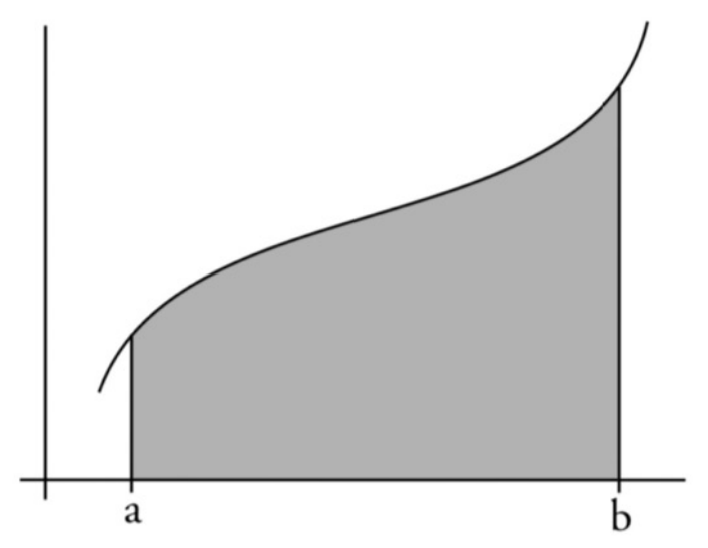
\includegraphics[width=6.5cm]{Capture25}\\
\centering
\text{\textbf{Figure:} Area under a curve}
\end{figure}\\
The notation we use to describe this is the \textit{definite integral}
\begin{equation*}
\int_a^bf(x)dx
\end{equation*}
Unlike an \textit{indefinite} integral, a definite integral has specified
start and end points.
The idea of discretised rectangles is illustrated here:
\begin{figure}[h]
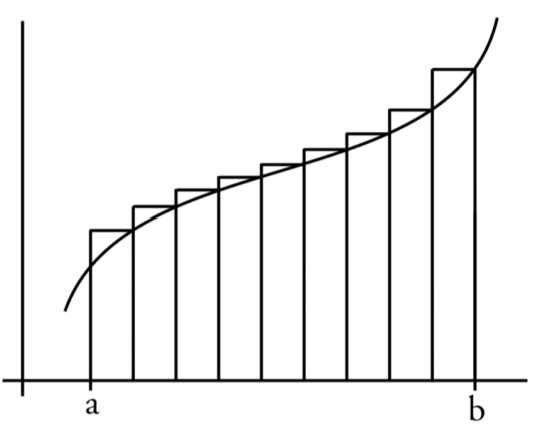
\includegraphics[width=6.5cm]{Capture26}\\
\centering
\text{\textbf{Figure:} Area under curve divided into rectangles}
\end{figure}\\
The idea here is to take the cumulative area of the rectangles as
their width becomes infinitesimally small.\\
(next page)
\newpage
\noindent\textbf{Intuition}\\
Consider the curve $f(x)=x^2$, where we add up the area under
the curve from point $a=0$ to point $b$:
\begin{figure}[h]
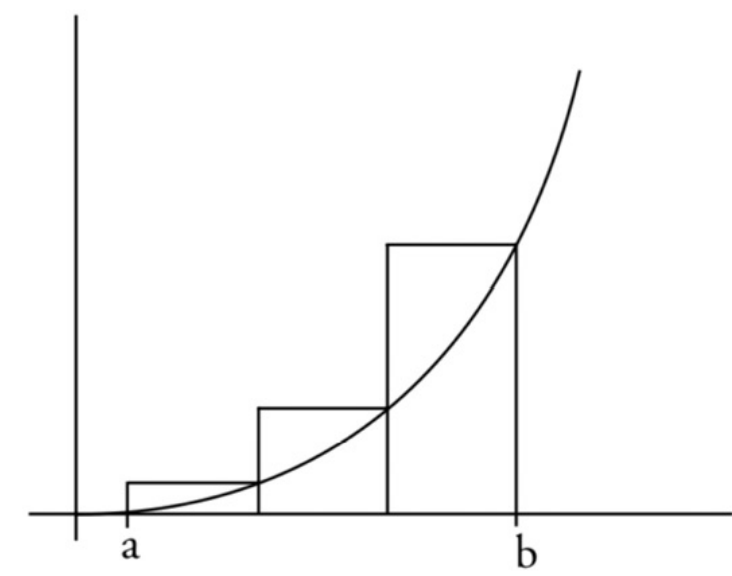
\includegraphics[width=8cm]{Capture27}\\
\centering
\text{\textbf{Figure:} $\int_a^bf(x)dx$ approximated by 3 rectangles}
\end{figure}\\
The interval from $a=0$ to $b$ is subdivided into $n$ sections; the above figure illustrates $n=3$. 
Each subdivision forms the base of a rectangle, with the top of each rectangle touching the graph;
here we choose to have the intersection of each rectangle and the graph be at the
upper right hand of the rectangle. This causes the cumulative area of the rectangles
to be larger than the actual area under the curve.\\
\vspace{1mm}\\
Now we add up the areas of the rectangles to get an
approximation of the area under the curve:
\begin{equation*}
\underbrace{\left(\frac{b}{n}\right)}_{\text{base}}
\underbrace{\left(\frac{b}{n}\right)^2}_{\text{height}}
+\left(\frac{b}{n}\right)\left(\frac{2b}{n}\right)^2
+\left(\frac{b}{n}\right)\left(\frac{3b}{n}\right)^2
+\ldots+\left(\frac{b}{n}\right)\left(\frac{nb}{n}\right)^2
\end{equation*}
First we simplify by factoring out $\left(\frac{b}{n}\right)^3$:
\begin{align*}
\left(\frac{b}{n}\right)\left(\frac{b}{n}\right)^2+&
\left(\frac{b}{n}\right)\left(\frac{2b}{n}\right)^2+
\left(\frac{b}{n}\right)\left(\frac{3b}{n}\right)^2+
\ldots+\left(\frac{b}{n}\right)\left(\frac{nb}{n}\right)^2\\
&=\left(\frac{b}{n}\right)^3(1+2^2+\ldots+(n-1)^2+n^2)
\end{align*}
Next we use geometry to simplify this\\
(next page)
\newpage
\noindent Consider a pyramid made up of a $n$ by $n$ by 1 base, 
followed by a $(n-1)$ by $(n-1)$ by 1 layer, and so on until it has a height $n$.
\begin{figure}[h]
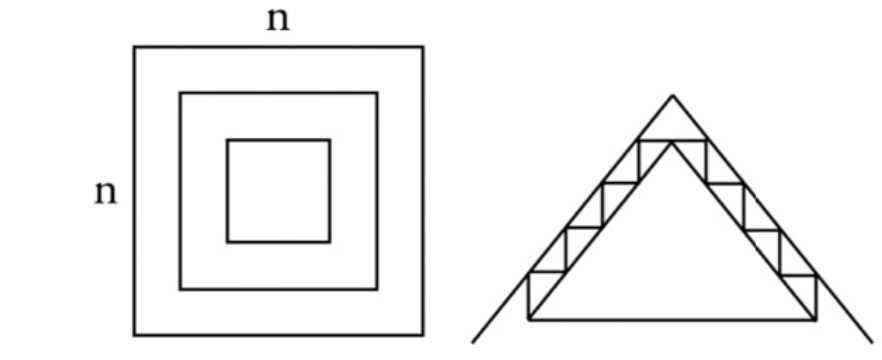
\includegraphics[width=9cm]{Capture28}\\
\centering
\text{\textbf{Figure:} Top and side views of proposed pyramid}
\end{figure}\\
The volume of the pyramid is $(1^2+2^2+\ldots+(n-1)^2+n^2)$. 
Now consider the largest pyramid that can fit inside our proposed structure; it would
have a volume of $\frac{1}{3}$ $\cdot$ base $\cdot$ height=$\frac{1}{3}n^3$. This gives us the inequality
\begin{equation*}
\frac{1}{3}n^3<1^2+2^2+\ldots+(n-1)^2+n^2
\end{equation*}
Finally, consider the the smallest ordinary pyramid that could contain our proposed structure;
it would have a base and height of $n+1$, giving it a volume of $\frac{1}{3}(n+1)^3$,
completing our inequality:
\begin{equation*}
\frac{1}{3}n^3<1^2+2^2+\ldots+(n-1)^2+n^2
<\frac{1}{3}(n+1)^3
\end{equation*}
Dividing throughout by $n^3$ gives us
\begin{equation*}
\frac{1}{3}<\frac{1^2+2^2+\ldots+(n-1)^2+n^2}{n^3}
<\frac{1}{3}\cdot\left(\frac{n+1}{n}\right)^3
=\frac{1}{3}\left(1+\frac{1}{n}\right)^3
\end{equation*}
Since $\lim_{n\to\infty}\left(1+\frac{1}{n}\right)=1$
\begin{equation*}
\lim_{n\to\infty}\frac{1^2+2^2+\ldots+(n-1)^2+n^2}{n^3}=\frac{1}{3}
\end{equation*}
Thus, going back to our original problem:
\begin{align*}
\left(\frac{b}{n}\right)^3(1+2^2+\ldots+(n-1)^2+&n^2)
=b^3\left(\frac{1+2^2+\ldots+(n-1)^2+n^2}{n^3}\right)
=\frac{1}{3}b^3
\end{align*}
This leads us to the result:
\begin{equation*}
\int_0^bx^2dx=\frac{1}{3}b^3
\end{equation*}
\newpage

\subsection{Riemann Sums} %010624
Here we define a Riemann Sum. An intuitive way to find a definite integral 
$\int_a^bf(x)\,dx$ is by approximating the area under a curve using sums
of rectangles.
\begin{figure}[h]
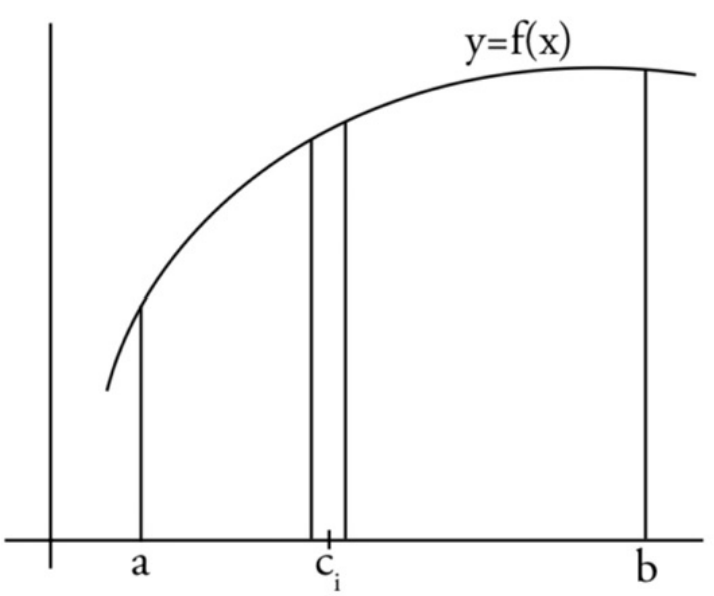
\includegraphics[width=8cm]{Capture29}\\
\centering
\text{\textbf{Figure:} Area under a curve}
\end{figure}\\
With this we can come up with a general procedure:
\begin{itemize}
\item Divide $[a,b]$ into $n$ equal pieces of length 
$\Delta x=\frac{b-a}{n}$.
\item Pick \textit{any} $c_i$ in the $i^{\text{th}}$ interval and use $f(c_i)$
to compute the height for each rectangle.
\item Sum the areas of the rectangles:
\begin{align*}
\underbrace{f(c_1)}_{\text{height}}\underbrace{(\Delta x)}_{\text{base}}
+f(c_2)&\Delta x+\ldots+f(c_{n-1})\Delta x+f(c_n)\Delta x\\
&=\sum_{i=1}^nf(c_i)\Delta x
\end{align*}
\end{itemize}
The sum $\sum_{i=1}^nf(c_i)\Delta x$ is called a \textbf{Riemann Sum}.\\
\vspace{1mm}\\
As $n$ approaches infinity, the sum approaches the value of a definite integral:
\begin{equation*}
\sum_{i=1}^nf(c_i)\Delta x=\int_a^bf(x)\,dx
\end{equation*}
Which is the area under the curve $f(x)$ above the interval $[a,b]$.
\newpage

\subsection{Introduction to Fundamental theorem of Calculus (FTC1)} %010624
Here we introduce the fundamental theorem of calculus.
There are two versions of it so we abbreviate them as
FTC1 and FTC2. Here we cover FTC1.\\
\vspace{1mm}\\
\textbf{Theorem:} If $f(x)$ is continuous and $F'(x)=f(x)$, then:
\begin{equation*}
\int_a^bf(x)\,dx=F(b)-F(a)
\end{equation*}
Recall the notation of the antiderivative:
\begin{equation*}
F(x)=\int f(x)\,dx
\end{equation*}
The FTC1 can also be written as
\begin{equation*}
\int_a^bf(x)\,dx=F(x)|_a^b
\end{equation*}
\textbf{Example:} Consider $f(x)=x^2$, using FTC we get:
\begin{equation*}
\int_a^bx^2dx=\int_a^bf(x)\,dx=F(b)-F(a)=
\frac{b^3}{3}-\frac{a^3}{3}
\end{equation*}
By using the FTC we avoid the elaborate computation required by Riemann sums.
\newpage

\subsection{Properties of Integrals} %010624
Here we list a number of properties of integrals. Most are intuitive:\\
\vspace{1mm}\\
1. The integral of a sum is the sum of integrals
\begin{equation*}
\int_a^b(f(x)+g(x))\,dx=\int_a^bf(x)\,dx+\int_a^bg(x)\,dx
\end{equation*}
2. Constant multiples can be factored out:
\begin{equation*}
\int_a^bcf(x)\,dx=c\int_a^bf(x)\,dx
\end{equation*}
(scaling the area under a graph by a multiple is the same as scaling the graph
itself by the multiple then finding the area under it)\\
\vspace{1mm}\\
3. We can combine definite integrals; if $a<b<c$ then
\begin{equation*}
\int_a^bf(x)\,dx+\int_b^cf(x)\,dx=\int_a^cf(x)\,dx
\end{equation*}
Graphically:
\begin{figure}[h]
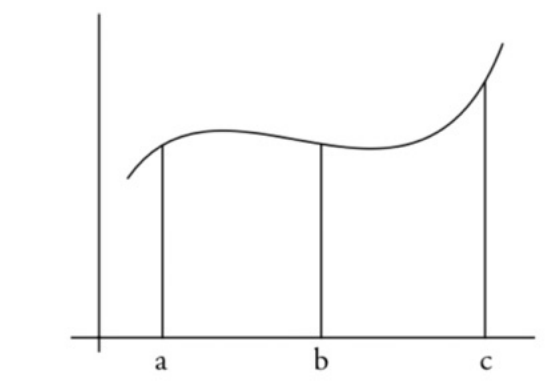
\includegraphics[width=8cm]{Capture30}\\
\centering
\text{\textbf{Figure:} Combining two areas under a curve}
\end{figure}\\
4. A definite integral over a range of length 0 is 0:
\begin{equation*}
\int_a^af(x)\,dx=0
\end{equation*}
(next page)
\newpage
\noindent5. Taking the upper limit to be lower than the lower limit:
\begin{equation*}
\int_a^bf(x)\,dx=-\int_b^af(x)\,dx
\end{equation*}
(Since $F(b)-F(a)=-(F(a)-F(b))$)\\
\vspace{1mm}\\
6. \textit{Estimation}: If $f(x)\leq g(x)$ and $a<b$, then
\begin{equation*}
\int_a^bf(x)\,dx\leq\int_a^bg(x)\,dx
\end{equation*}
7. \textit{Substitution/Change of variables}: In terms of indefinite integrals,
if $u=u(x)$ then $du=u'(x)\,dx$ and 
$\int g(u)\,du=\int g(u(x))u'(x)\,dx$ (substitution).
We can apply this concept to definite integrals by adapting the limits accordingly:
\begin{equation*}
\int_{u_1}^{u_2}g(u)\,du=\int_{x_1}^{x_2}g(u(x))u'(x)\,dx
\end{equation*}
where $u_1=u(x_1)$ and $u_2=u(x_2)$. Note that this is true if $u$ is always increasing 
or always decreasing on $x_1<x<x_2$ (the variables $u$ and $x$ must be one-to-one 
or a value of $u$ can correspond to multiple values of $x$ or vice-versa.)\\
\vspace{1mm}\\
\textbf{Example of Substitution/Change of variables}:\\
Consider $\int_1^2(x^3+2)^5x^2dx$, we attempt to find the result by substitution. 
Here we use $u=x^3+2$, taking the limits into account; 
we have $du=3x^2dx$, $u(1)=3$ and $u(2)=10$. This gives us:
\begin{align*}
\int_{x=1}^{x=2}(x^3+2)^5x^2dx
&=\int_{u=3}^{u=10}u^5\frac{1}{3}du\\
&=\left.\frac{u^6}{6\cdot3}\right|_{u=3}^{u=10}\\
&=\frac{1}{18}(10^6-3^6)
\end{align*}
\newpage

\subsection{The Fundamental Theorem and the Mean Value Theorem} %020624
Here we compare the FTC1 with the Mean Value Theorem (MVT).
Substituting $\Delta F=F(b)-F(a)$ and $\Delta x=b-a$, the FTC1 tells us that:
\begin{equation*}
\Delta F=\int_a^bf(x)\,dx
\end{equation*}
Dividing both sides by $\Delta x$:
\begin{equation*}
\frac{\Delta F}{\Delta x}
=\underbrace{\frac{1}{b-a}\int_a^bf(x)\,dx}_{\text{Average$(f)$}}
\end{equation*}
Consider the Riemann sum:
\begin{equation*}
\int_0^nf(x)\,dx\approx f(1)+f(2)+\ldots+f(n)
\end{equation*}
Which is a cumulative sum of the values of $f(x)$ over a specified range;
this means that
\begin{align*} 
\frac{\int_0^nf(x)\,dx}{n}&\approx
\frac{f(1)+f(2)+\ldots+f(n)}{n}\\
&=\text{Average}(f)
\quad\text{(Over the specified range)}
\end{align*}
Going back to the original problem, this means that:
\begin{align*}
\frac{\Delta F}{\Delta x}
&=\frac{1}{b-a}\int_a^bf(x)\,dx\\
&=\text{Average}(F')
\quad\text{(Over a range from $a$ to $b$)}
\end{align*}
Rearranging:
\begin{equation*}
\Delta F=\text{Average}(F')\Delta x
\end{equation*}
Compare this with the MVT, which gives us
\begin{align*}
\frac{\Delta F}{\Delta x}=\frac{F(b)-F(a)}{b-a}
&=F'(c)\quad\text{For some $c$ where $a\leq c\leq b$}\\
\Delta F&=F'(c)\Delta x
\end{align*}
(next page)
\newpage
\noindent The FTC1 and MVT give us:
\begin{align*}
\text{MVT:}\quad\Delta F&=F'(c)\Delta x\\
\text{FTC1:}\quad\Delta F&=\text{Average}(F')\Delta x
\end{align*}
The value of Average($F'$) in the first fundamental theorem is very specific, 
while $F'(c)$ from the mean value theorem is not, since all we know is $a\leq c\leq b$.\\
\vspace{1mm}\\
For the MVT, even though we don't know what $c$ is, we can say that
\begin{align*}
\left(\min_{a<x<b}F'(x)\right)\leq&F'(c)
\leq\left(\max_{a<x<b}F'(x)\right)\\
\left(\min_{a<x<b}F'(x)\right)\Delta x\leq F'(c)&\Delta x
=\Delta F\leq\left(\max_{a<x<b}F'(x)\right)\Delta x
\end{align*}
Notice that the FTC1 allows us to make the same deduction, but with a much more
specific function Average($F'$)
\begin{align*}
\left(\min_{a<x<b}F'(x)\right)\leq\text{Average}(F')&
\leq\left(\max_{a<x<b}F'(x)\right)\\
\left(\min_{a<x<b}F'(x)\right)\Delta x\leq\text{Average}(F')\Delta x&
=\Delta F\leq\left(\max_{a<x<b}F'(x)\right)\Delta x
\end{align*}
The fundamental theorem of calculus is clearly much stronger than the MVT, allowing us
to abandon the mean value theorem, since either theorem gives us the same conclusion
\begin{equation*}
\left(\min_{a<x<b}F'(x)\right)\Delta x\leq
\Delta F\leq\left(\max_{a<x<b}F'(x)\right)\Delta x
\end{equation*}
\newpage

\subsection{Second Fundamental Theorem of Calculus} %040624
Here we introduce the Second Fundamental Theorem of Calculus. These two theorems are 
key to finding the intuition toward the relationship between integrals and derivatives.\\
\vspace{1mm}\\
\textbf{Theorem:} If $f$ is continuous and 
$G(x)=\int_{a}^xf(t)\,dt$, then $G'(x)=f(x)$.\\
\vspace{1mm}\\
\textbf{Intuition}\\
The variable $t$ is a dummy variable. What matters here is the upper limit---$x$.
The upper limit of the integral is \textit{changing with respect to $x$}.
This is the link between the area under a curve (integrals) and the change with
respect to $x$ (derivatives). See below (\ref{fundamentals:integrals:FTC_proof}).

\subsection{Intuition and proofs---Fundamental\\Theorem of Calculus} %050624
\label{fundamentals:integrals:FTC_proof}
\textbf{Second Fundamental Theorem}\\
Recall the FTC2: If $f$ is continuous and 
$F(x)=\int_{a}^xf(t)\,dt$, then $F'(x)=f(x)$. Here we use the interpretation 
that $F(x)$ equals the area under the curve from $a$ to $x$, taking its derivative 
to show that its equal to $f$. This links the idea of the integral and the derivative.
\begin{figure}[h]
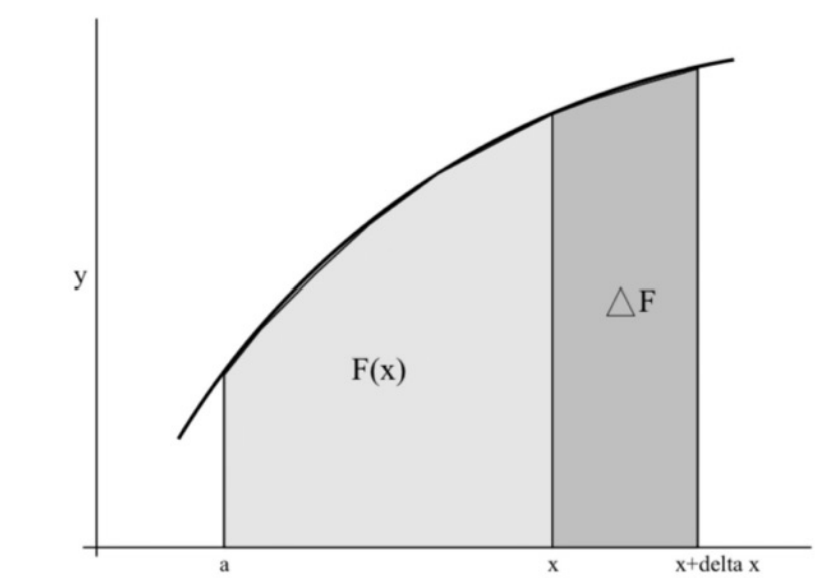
\includegraphics[width=8cm]{Capture31}\\
\centering
\text{\textbf{Figure:} Graph of $f(x)$ with shaded area $F(x)$}
\end{figure}\\
As $\Delta x$ becomes smaller, we can apporximate $\Delta F$ to be a rectangle of 
width $\Delta x$ and height $f(x)$. So
\begin{equation*}
\Delta F\approx \Delta xf(x)
\end{equation*}
So as $\Delta x\to0$:
\begin{equation*}
F'(x)=\lim_{\Delta x\to0}\frac{\Delta F}{\Delta x}=f(x)
\end{equation*}
(next page)
\newpage
\noindent\textbf{First Fundamental Theorem}\\
\textbf{Theorem:} (First Fundamental Theorem of Calculus) If $f$ is continuous and
$F'=f$, then $\int_a^bf(x)\,dx=F(b)-F(a)$.\\
\vspace{1mm}\\
Here we define an antiderivative $G$ of $f$ before using it to calculate
$F(b)-F(a)$. We start with $F'=f$, where $f$ is continuous (not strictly necessary, but 
allows us to use FTC2). Now consider $G(x)=\int_a^xf(t)\,dt$; by FTC2:
\begin{equation*}
G'(x)=f(x)
\end{equation*}
So $F'(x)=G'(x)=f(x)$. This means that $F$ and $G$ differ only by a constant:
\begin{equation*}
F(x)=G(x)+c
\end{equation*} 
Now we can show:
\begin{align*}
F(b)-F(a)&=(G(b)+c)-(G(a)+c)\\
&=G(b)-G(a)\\
&=\int_a^bf(t)\,dt-\int_a^af(t)\,dt\\
&=\int_a^bf(t)\,dt-0\\
F(b)-F(a)&=\int_a^bf(x)\,dx
\end{align*}
\newpage

\subsection{Integrals and Averages} %050624
Here we show how integrals can act as continous analogues of averages. Consider
finding the average value of a function $y-f(x)$ on an interval:
\begin{align*}
\text{Discrete Average}&\approx\frac{y_1+y_2+\ldots+y_n}{n}\\
\text{Continuous Average}&=\frac{1}{b-a}\int_a^bf(x)\,dx=\text{Ave}(f)
\end{align*} 
The continous average is essentially the discrete average as the number of values $n$ 
approaches infinity.\\
\vspace{1mm}\\
\textbf{Intuition}\\
Consider $f(x)$ over an interval $[a,b]$:
\begin{figure}[h]
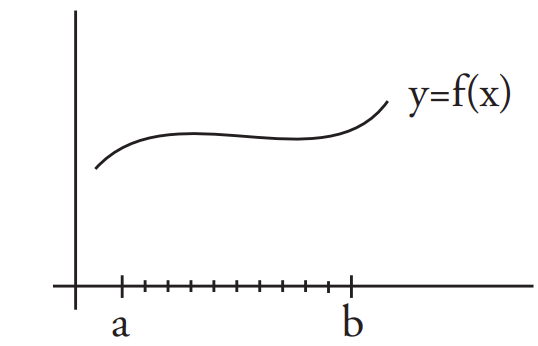
\includegraphics[width=8cm]{Capture32}\\
\centering
\text{\textbf{Figure:} $f(x)$ over $[a,b]$}
\end{figure}\\
Consider $n+1$ equally spaced points where $a=x_0<x_1<\ldots<x_n=b$
with the distance between each point being $\Delta x=\frac{b-a}{n}$. 
For $y_i=f(x_i)$, the Riemann sum approximating the area under $f$ over 
the specified range would be
\begin{equation*}
(y_0+y_1+\ldots+y_n)\Delta x
\end{equation*}
As $n\to\infty$, the Riemann sum approaches the area under the curve, 
\begin{equation*}
\int_a^bf(x)\,dx
\end{equation*}
(next page)
\newpage
\noindent Now we can show, as $n\to\infty$
\begin{align*}
\int_a^bf(x)\,dx&\approx(y_0+y_1+\ldots+y_n)\Delta x\\
\frac{1}{b-a}\int_a^bf(x)\,dx&\approx
\frac{1}{b-a}(y_0+y_1+\ldots+y_n)\Delta x\\
&=\frac{1}{b-a}(y_0+y_1+\ldots+y_n)\frac{b-a}{n}\\
\frac{1}{b-a}\int_a^bf(x)\,dx&\approx\frac{y_0+y_1+\ldots+y_n}{n}
\end{align*}
\textbf{Weighted averages}\\
Similarly, continuous \textit{weighted averages} are given by
\begin{equation*}
\frac{\int_a^b f(x)w(x)\,dx}{\int_a^b w(x)\,dx}
\end{equation*}
Where a discrete analogue might look like
\begin{equation*}
\frac{10w_1+20w_2+30w_3}{w_1+w_2+w_3}
\end{equation*}
\newpage

\subsection{Introduction---Numerical Integration} %060624
Many functions may not have easily describable antiderivatives, so many integrals
must be approximated by a computer/calculator. The simplest of these
techniques is Riemann Sums:\\
\vspace{1mm}\\
\textbf{Riemann Sums in numerical integration}\\
Riemann Sums approximate the area between the area between the $x$-axis and the 
curve over the interval $[a,b]$ by a sum of areas of rectangles:
\begin{figure}[h]
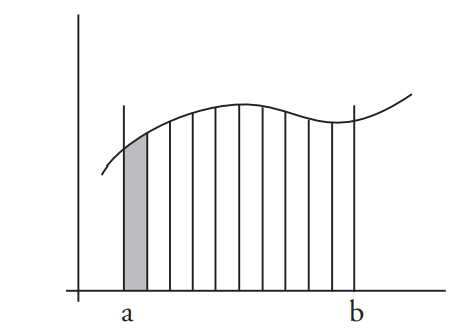
\includegraphics[width=8cm]{Capture33}\\
\centering
\text{\textbf{Figure:} Riemann sum of $f(x)$ over $[a,b]$}
\end{figure}\\
Each rectangle has a width $\Delta x=x_i-x_{i-1}$. There
are $n$ rectangles whose top edges have $x$-coordinates 
$a=x_0<x_1<\ldots<x_n=b$; the heights of the rectangles are therefore 
$y_0=f(x_0),y_1=f(x_1),\ldots,y_n=f(x_n)$.
Note that one can use either left or right Riemann sums to approximate the area. 
The formula for the left Riemann sum, where the top
left corner of each rectangle is set at the height of the graph, is
\begin{equation*}
(y_0+y_1+\ldots+y_{n-1})\Delta x
\end{equation*}
Similarly, if we left the top right corner of each rectangle be set to the
height of the graph we get the right Riemann sum:
\begin{equation*}
(y_1+y_2+\ldots+y_n)\Delta x
\end{equation*}
In the end both act as (inefficient) approximations to
\begin{equation*}
\int_a^bf(x)\,dx
\end{equation*}
\newpage

\subsection{Numerical Integration---Trapezoidal Rule} %060624
Similar to Numerical integration by Riemann sums, the Trapezoidal rule
divides the area under the graph into trapezoids (using segments of secant lines)
rather than rectangles (Riemann sums).
\begin{figure}[h]
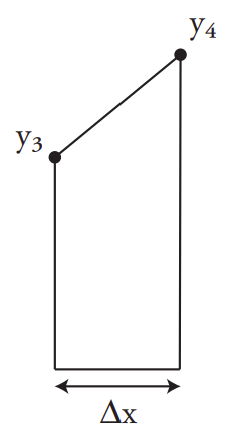
\includegraphics[width=3.2cm]{Capture34}
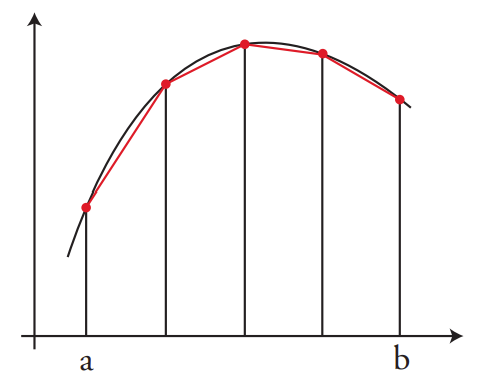
\includegraphics[width=6.8cm]{Capture35}\\
\centering
\begin{align*}
\text{\textbf{Left:}}&\text{ Single trapezoid}\\
\text{\textbf{Right:}}&\text{ Trapezoids approximate integral more accurately}
\end{align*}
\end{figure}\\
The trapezoids are able to approximate the area under the curve more accurately. 
Each trapezoid has a width $\Delta x=x_i-x_{i-1}$ where there
are $n$ trapezoids whose bottom edges have $x$-coordinates 
$a=x_0<x_1<\ldots<x_n=b$. The heights of each trapezoid are $y_{i-1}$ and $y_i$
where $y_{i}=f(x_i)$.\\
\vspace{1mm}\\
Trapezoid $i$ has area 
\begin{equation*}
\Delta x\left(\frac{y_{i-1}+y_i}{2}\right)
\end{equation*}
Adding up the areas of all the trapezoids we get
\begin{align*}
\text{Area}&=\Delta x\left(\frac{y_0+y_1}{2}+
\frac{y_1+y_2}{2}+\ldots+\frac{y_{n-1}+y_n}{2}\right)\\
&=\Delta x\left(\frac{y_0}{2}+y_1+y_2+\ldots+y_{n-1}+
\frac{y_n}{2}\right)
\end{align*}
Notice that the trapezoidal rule is the average of the left and right
Riemann sums. It is much better than a Riemann sum, but is still not very efficient.
\newpage

\subsection{Numerical Integration---Simpson's rule} %090624
\textbf{Intuition:}\\
Here we introduce Simpson's rule, which is similar to Riemann sum and Trapezoid rule 
approximation, but instead approximates $f(x)$ using parabolas instead of horizontal
or secant lines.\\
\vspace{1mm}\\
Same with the former two approximations, we divide the range we want to approximate 
into $n$ intervals, with the base of each interval being $\Delta x=x_i-x_{i-1}$.
We use the corresponding $y_i=f(x_i)$ to fit a parabola to the curve at each interval.	
\begin{figure}[h]
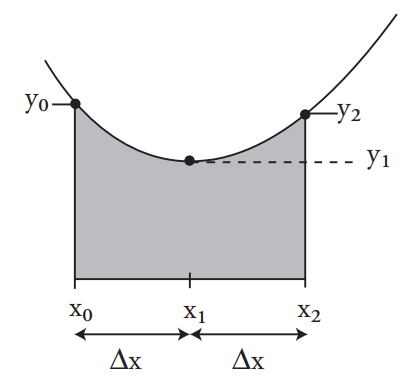
\includegraphics[width=4.7cm]{Capture36}
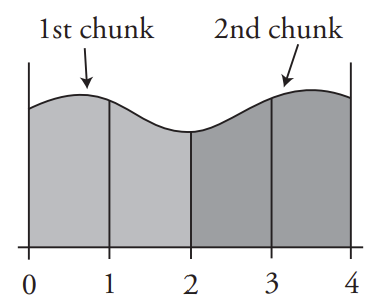
\includegraphics[width=5.3cm]{Capture37}\\
\centering
\begin{align*}
\text{\textbf{Left:}}&\text{ Parabolic approximation over two intervals/one chunk}\\
\text{\textbf{Right:}}&\text{ Simpson's rule for $n$ intervals ($n$ must be even)}
\end{align*}
\end{figure}\\
Notice we fit a parabola over an interval of $2\Delta x$, and therefore
require an \textit{even} number of intervals over the range we are approximating. Each 'chunk' of two intervals has the area:
\begin{equation*}
\frac{\Delta x}{3}(y_0+4y_1+y_2)
\end{equation*}
The area of all $n$ chunks summed up gives us the total estimate of the area:
\begin{equation*}
\int_a^bf(x)\,dx\approx \frac{\Delta x}{3}(y_0+4y_1+2y_2
+4y_3+2y_4+\ldots+2y_{n-2}+4y_{n-1}+y_n) 
\end{equation*}
\newpage

\subsection{Simpson's rule---Derivation} %070624
Here we derive the formula for Simpson's rule, a method for Numerical integration:
\begin{equation*}
\int_a^bf(x)\,dx\approx \frac{\Delta x}{3}(y_0+4y_1+2y_2
+4y_3+2y_4+\ldots+2y_{n-2}+4y_{n-1}+y_n) 
\end{equation*}
The area under our function is divided into an even number of intervals 
as shown, approximation occurs in 'chunks', which is equivalent to 2 intervals:
\begin{figure}[h]
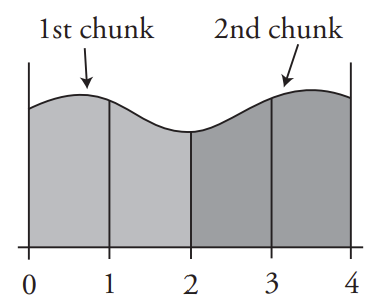
\includegraphics[width=6cm]{Capture37}\\
\centering
\text{\textbf{Figure:} Each chunk is made up of two intervals}
\end{figure}\\
First we derive the equation for the area of each 'chunk' approximating the area of
one of $n$ segments:
\begin{equation*}
\frac{\Delta x}{3}(y_0+4y_1+y_2)
\end{equation*}
Each 'chunk' is equal to the width of two intervals/$2\Delta x$:
\begin{figure}[h]
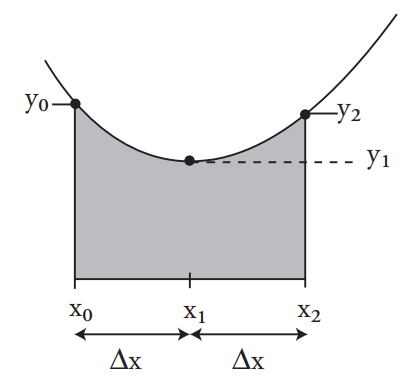
\includegraphics[width=5cm]{Capture36}\\
\centering
\text{\textbf{Figure:} We use three points to approximate a parabola over two $\Delta x$}
\end{figure}\\
(Notice that we fit a parabola over an interval of $2\Delta x$, and therefore
require an \textit{even} number of intervals over the range we are approximating.)\\
(next page)
\newpage
\noindent Our approximation $P(x)$ for the upper edge of our area has the formula:
\begin{equation*}
P(x)=ax^2+bx+c
\end{equation*}
Thus we require three points. Taking $x_1$ to be 0 (this can be done since we only care
about estimating the area below a parabola made of our three $y_i$),
our area can be expressed as:
\begin{equation*}
\text{Area}=\int_{-\Delta x}^{\Delta x}P(x)\,dx=\int_{-\Delta x}^{\Delta x}ax^2+bx+c\,dx
\end{equation*}
\begin{figure}[h]
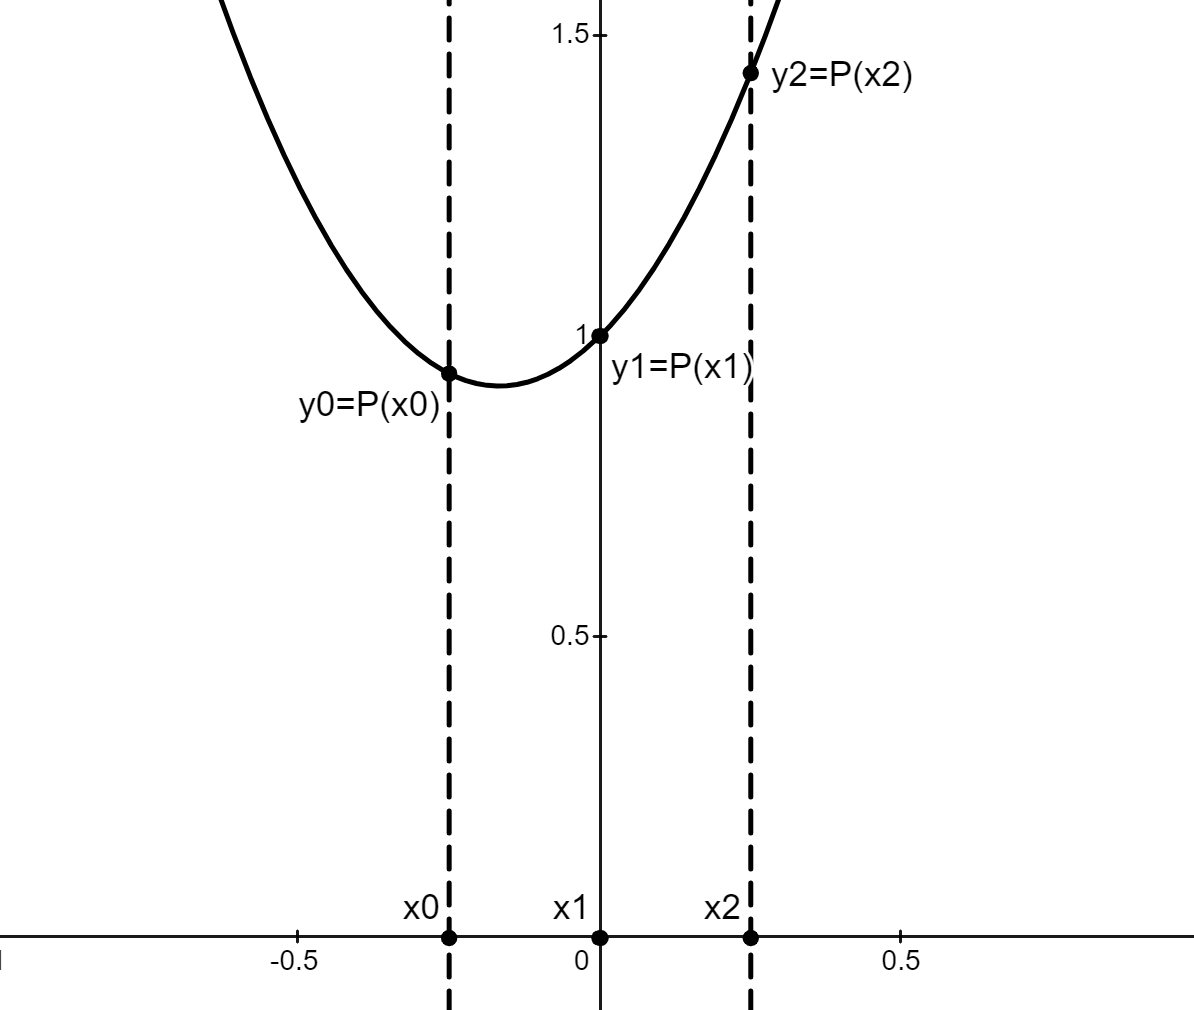
\includegraphics[width=6cm]{Capture38}\\
\centering
\text{\textbf{Figure:} Our points shifted such that $x_1=0$}
\end{figure}\\
Simplifying our integral:
\begin{align*}
\text{Area}=\int_{-\Delta x}^{\Delta x}ax^2+b&x+c\,dx
=\left.\frac{a}{3}x^3-\frac{b}{2}x^2+cx\right|^{\Delta x}_{-\Delta x}\\
&=\frac{2}{3}a(\Delta x)^3+2c\Delta x
\end{align*}
Since we have $x_1=0$, $P(x_1)=P(0)=y_1=c$. This means
\begin{align*}
\text{Area}=\frac{2}{3}a(\Delta x)^3+2c\Delta x
&=\frac{2}{3}a(\Delta x)^3+2y_1\Delta x\\
&=\frac{\Delta x}{3}(2a(\Delta x)^2+6y_1)
\end{align*}\\
(next page)
\newpage
\noindent Since
\begin{align*}
P(\Delta x)&=a(\Delta x)^2+b\Delta x+c=y_2\\
P(-\Delta x)&=a(\Delta x)^2-b\Delta x+c=y_0
\end{align*}
and $y_1=c$, we can also show
\begin{align*}
2a(\Delta x)^2+2c&=y_0+y_2\\
2a(\Delta x)^2&=y_0+y_2-2y_1
\end{align*}
Therefore, returning to finding the area under our single chunk:
\begin{align*}
\text{Area}&=\frac{\Delta x}{3}(2a(\Delta x)^2+6y_1)\\
&=\frac{\Delta x}{3}(y_0+y_2-2y_1+6y_1)\\
&=\frac{\Delta x}{3}(y_0+4y_1+y_2)
\end{align*}
We add up the chunks to get the approximated value of our integral:
\begin{equation*}
\text{Total Area}=\frac{\Delta x}{3}
[(y_0+4y_1+y_2)+(y_2+4y_3+y_4)+\ldots+(\ldots y_n)]
\end{equation*}
With that we get the final form of Simpson's rule
\begin{equation*}
\int_a^bf(x)\,dx\approx \frac{\Delta x}{3}(y_0+4y_1+2y_2
+4y_3+2y_4+\ldots+2y_{n-2}+4y_{n-1}+y_n) 
\end{equation*} 
\newpage 

\subsection{Area under Bell Curve}%110624
Here we prove the value
\begin{equation*}
\int^{\infty}_0e^{-x^2}dx=\frac{\sqrt{\pi}}{2}
\end{equation*}
\textbf{Volume about vertical axis:}\\
Consider the volume of revolution created by rotating the curve $e^{-r^2}$ around the \textit{vertical} axis:
\begin{equation*}
V=\int^{\infty}_02\pi re^{-r^2}dr
\end{equation*}
(Think of it as a Riemann sum of circular 3-dimensional strips around the vertical axis,
with each strip having circumference $2\pi r$, height $e^{-r^2}$ and thickness $dr$). 
This evaluates to:
\begin{align*}
V&=\int^{\infty}_02\pi re^{-r^2}dr\\
&=\left.-\pi e^{-r^2}\right|_0^\infty\\
&=\pi
\end{align*}
\textbf{Area under curve:}\\
We aim to find the volume under the entire curve:
\begin{equation*}
Q=\int_{-\infty}^{\infty}e^{-t^2}dt
\end{equation*}
Illustrated:
\begin{figure}[h]
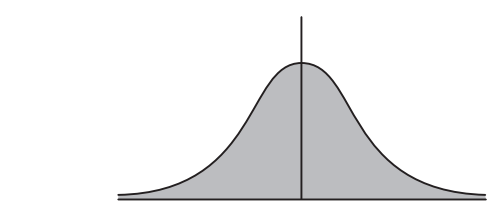
\includegraphics[width=6cm]{Capture39}\\
\centering
\text{\textbf{Figure:} $Q$=Area under $e^{-t^2}$}
\end{figure}\\
Now we show that
\begin{align*}
Q^2&=V=\pi\\
Q&=\sqrt{\pi}
\end{align*}
(next page)
\newpage
\noindent We prove that $V=Q^2$ using slices; imagine 3-dimsntional slices of our 
revolution of $e^{-r^2}$ about the vertical axis:
\begin{figure}[h]
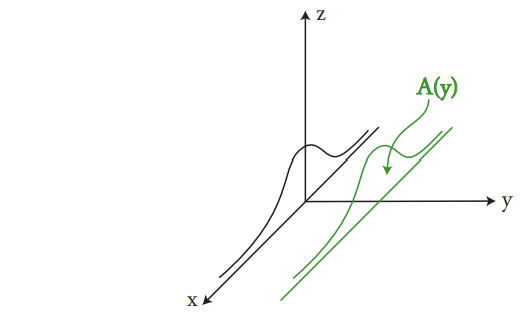
\includegraphics[width=6cm]{Capture40}\\
\centering
\text{\textbf{Figure:} Three dimensional slices of the volume of rotation of $e^{-r^2}$}
\end{figure}\\
Where each slice has an area $A(y)$.
Here we slice along the $y$-axis. We want an expression for $A(y)$, so we fix $y=b$ 
and vary $x$, using the pythagorean theorem to find $r$:
\begin{figure}[h]
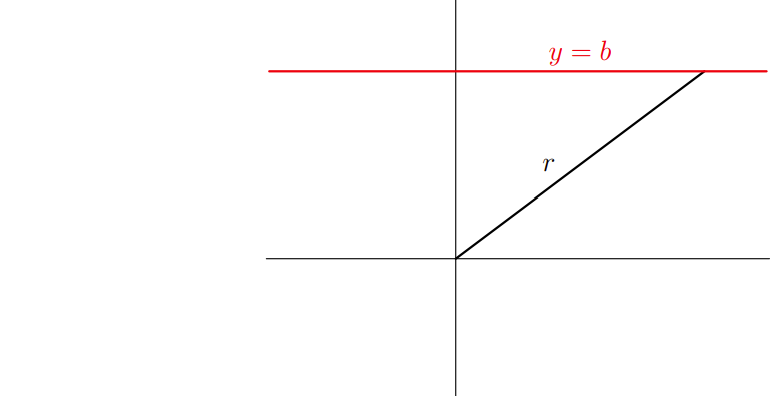
\includegraphics[width=6cm]{Capture41}\\
\centering
\text{\textbf{Figure:} Top down view of a single slice; $r^2=b^2+x^2$}
\end{figure}\\
The height of our slice follows the formula
\begin{equation*}
\text{Height}=e^{-r^2}=e^{-(b^2+x^2)}
\end{equation*}
The total volume of our slices is equal to $V$, and can be expressed as 
\begin{equation*}
V=\int_{-\infty}^{\infty}A(y)\,dy
\end{equation*}
With our $y$-coordinate fixed at $b$,
\begin{align*}
A(b)&=\int_{-\infty}^{\infty}e^{-(b^2+x^2)}dx\\
&=e^{-b^2}\int_{-\infty}^{\infty}e^{-x^2}dx\\
&=e^{-b^2}Q
\end{align*}
(next page)
\newpage
\noindent Since
\begin{equation*}
A(b)=e^{-b^2}Q
\end{equation*}
And our volume is given by
\begin{equation*}
V=\pi=\int_{-\infty}^{\infty}A(y)\,dy
\end{equation*}
We can show
\begin{align*}
V&=\int_{-\infty}^{\infty}A(y)\,dy\\
&=\int_{-\infty}^{\infty}e^{-y^2}Q\,dy\\
&=Q\int_{-\infty}^{\infty}e^{-y^2}\,dy\\
&=Q^2\quad\text{(since $Q=\int^{\infty}_{-\infty}e^{-t^2}dt$)}
\end{align*}
With that we get 
\begin{align*}
\int^{\infty}_{-\infty}e^{-t^2}dt&=Q\\
&=\sqrt{V}\\
&=\sqrt{\pi}\\
\int^{\infty}_{0}e^{-t^2}dt&=\frac{\sqrt{\pi}}{2}
\end{align*}
\newpage

%%%%%%%%%%%%%%%%%%%%%%%%%%%%%%%
%% Techniques of Integration %%
%%%%%%%%%%%%%%%%%%%%%%%%%%%%%%%

\section{Techniques of Integration}

\subsection{Review of Trigonometric Identities ($\sin$ and $\cos$)} %110624
Here we review angle formulas, in particular
\begin{align*}
\cos^2\theta&=\frac{1+\cos(2\theta)}{2}\\
\sin^2\theta&=\frac{1-\cos(2\theta)}{2}
\end{align*}
Recall:
\begin{align*}
\sin^2\theta+\cos^2\theta&=1\\
\cos(2\theta)&=\cos^2\theta-\sin^2\theta\\
\sin(2\theta)&=2\sin\theta\cos\theta
\end{align*}
We can show
\begin{align*}
\cos(2\theta)&=\cos^2\theta-\sin^2\theta\\
&=\cos^2\theta-(1-cos^2\theta)\\
&=2\cos^2\theta-1\\
\cos^2\theta&=\frac{1+\cos(2\theta)}{2}
\end{align*}
We can further show
\begin{align*}
\sin^2\theta&=1-\cos^2\theta\\
&=1-\left(\frac{1+\cos(2\theta)}{2}\right)\\
&=\frac{1-\cos(2\theta)}{2}
\end{align*}
\newpage

\subsection{Integral of $\sin^nx\cos^mx$---Part 1 (Odd Exponents)} %110624
Here we derive more complicated formulas involving integrals of the form:
\begin{equation*}
\int\sin^nx\cos^mx\,dx
\end{equation*}
Where $m$ and $n$ are non-negative integers. The integral can be divided into two
cases. First we consider the easier case---where at least one exponent is odd.\\
\vspace{1mm}\\
\textbf{Example:} $m=1$, $\int\sin^nx\cos x$\\
The idea here is to integrate via substitution, where $u=\sin x$ so $du=\cos x\,dx$:
\begin{align*}
\int\sin^nx\cos x\,dx&=\int u^n\,du\\
&=\frac{u^n+1}{n+1}+c\\
&=\frac{\sin^{n+1}x}{n+1}+c
\end{align*}
\textbf{Example:} $\int\sin^3x\cos^2x\,dx$\\
Similar to the first example, one of the exponents is odd. We turn this integral into
one in which the odd exponent is 1 using trigonometric identities. In this case the 
odd exponent is on $\sin x$, so we use
\begin{equation*}
\sin^2x=1-\cos^2x
\end{equation*}
so we get
\begin{align*}
\int\sin^3x\cos^2x\,dx&=\int(1-\cos^2x)\cdot
\sin x\cos^2x\,dx\\
&=\int(\cos^2x-\cos^4x)\cdot\sin x\,dx
\end{align*}
Similarly, we substitute the $u=\cos x$, $du=-\sin x\,dx$ (notice this removes the single exponent function):
\begin{align*}
\int(\cos^2x-\cos^4x)\cdot\sin x\,dx
&=\int(u^4-u^2)\,du\\
&=\frac{u^5}{5}-\frac{u^3}{3}+c\\
&=\frac{\cos^5x}{5}-\frac{\cos^3x}{3}+c
\end{align*}
\newpage

\subsection{Integral of $\sin^nx\cos^mx$---Part 2 (Even Exponents)} %120624
Here we consider the harder case---
$\int\sin^nx\cos^mx\,dx$ where both exponents are even.
This case is harder by virtue of being more tedious; it is solved by repeatedly applying
angle formulas rather than integration by substitution.\\
\vspace{1mm}\\
\textbf{Example:} $\int\cos^2x\,dx$\\
This example illustrates that the antiderivative for $\cos^2x$ is not straight forward:
\begin{align*}
\int\cos^2x\,dx&=\int\frac{1+\cos(2x)}{2}dx\\
&=\frac{x}{2}-\frac{\sin(2x)}{4}+c
\end{align*}
\textbf{Example:} $\int\sin^2x\cos^2x\,dx$\\
We use angle formulas to turn our \textit{product} of functions into \textit{sums}:
\begin{align*}
\sin^2x\cos^2x\,dx&=\left(\frac{1-\cos(2x)}{2}\right)
\cdot\left(\frac{1+\cos(2x)}{2}\right)\\
&=\frac{1-\cos^2(2x)}{4}\\
&=\frac{1}{4}-\frac{(1+\cos(4x))/2}{4}\\
&=\frac{1}{8}-\frac{\cos(4x)}{8}
\end{align*}
Our integral therefore looks like:
\begin{align*}
\int\sin^2x\cos^2x\,dx&=\int\frac{1}{8}-\frac{\cos(4x)}{8}dx\\
&=\frac{x}{8}-\frac{\sin(4x)}{32}+c
\end{align*}
(next page)
\newpage
\noindent Note that our example $\int\sin^2x\cos^2x\,dx$
can also be separated using
the other half angle formula
\begin{equation*}
\sin(2\theta)=2\sin\theta\cos\theta
\end{equation*}
we end up with the same expression 
\begin{align*} 
\sin^2x\cos^2x&=(\sin x\cos x)^2\\
&=\left(\frac{\sin(2x)}{2}\right)^2\\
&=\frac{\sin^2(2x)}{4}\\
&=\frac{1}{4}\left(\frac{1-\cos(4x)}{2}\right)\\
&=\frac{1}{8}-\frac{\cos(4x)}{8}
\end{align*}
\newpage

\subsection{Review of Trigonometric identities ($\tan$, $\sec$)} %150624
Here we briefly show
\begin{equation*}
\sec^2x=1+\tan^2x
\end{equation*}
this is apparent once we express $\sec$ in terms of $\sin$ and $\cos$:
\begin{align*}
\sec^2x&=\frac{1}{\cos^2x}\\
&=\frac{\cos^x+\sin^2x}{\cos^2x}\\
&=1+\tan^2x
\end{align*}

\subsection{Integration of $\tan$, $\sec$, $\csc$, $\cot$} %150624
\textbf{Integrating $\tan x$:}\\
Intuitively, we know
\begin{equation*}
\int\sec^2x\,dx=\tan x+c
\end{equation*}
This is relatively simple since it naturally falls out of the
derivative of $\tan x$. Here we derive the integral for $\tan x$:
\begin{equation*}
\int\tan x\,dx=-\ln|\cos x|+c
\end{equation*}
We express $\tan x$ in terms of $\sin x$ and $\cos x$ before 
substituting $u=\cos x$, $du=-\sin x\,dx$:
\begin{align*}
\int\tan x\,dx&=\int\frac{\sin x}{\cos x}dx\\
&=\int-\frac{1}{u}du\\
&=-\ln|u|+c\\
&=-\ln|\cos x|+c
\end{align*}
(next page)
\newpage
\noindent\textbf{Integrating $\cot x$:}\\
We show
\begin{equation*}
\int\cot x\,dx=-\ln|\sin x|+c
\end{equation*}
Substituting $u=\sin x$, $du=-\cos x\,dx$
\begin{align*}
\int\cot x\,dx&=\int\frac{\cos x}{\sin x}dx\\
&=\int-\frac{1}{u}du\\
&=-\ln|u|+c\\
&=-\ln|\sin x|+c
\end{align*}
\textbf{Integrating $\sec x$:}\\
We show
\begin{equation*}
\int\sec x\,dx=\ln|\sec x+\tan x|+c
\end{equation*}
Consider that
\begin{align*}
\frac{d}{dx}(\sec x+\tan x)&=\frac{\sin x}{\cos^2x}+\sec^2x\\
&=\sec x\tan x+\sec^2x\\
&=\sec x\cdot(\sec x+\tan x)
\end{align*}
Substituting $u=\sec x+\tan x$, notice
\begin{align*}
\frac{d}{dx}(\sec x+\tan x)&=\sec x\cdot(\sec x+\tan x)\\
\sec x&=\frac{\frac{d}{dx}(\sec x+\tan x)}{\sec x+\tan x}\\
&=\frac{u'}{u}=(\ln|u|)'
\end{align*}
Therefore we conclude
\begin{align*}
\sec x=(\ln|u|)'&=(\ln|\sec x+\tan x|)'\\
\int\sec x\,dx&=\ln|\sec x+\tan x|+c
\end{align*}
(next page)
\newpage
\noindent\textbf{Integrating $\csc x$:}\\
Here we show
\begin{equation*}
\int\csc x\,dx=\ln|\csc x-\cot x|+c
\end{equation*}
First note the derivatives of $\csc x$ and $\cot x$:
\begin{align*}
\frac{d}{dx}\csc x&=-\frac{\cos x}{\sin^2x}\\
&=-\csc x\cot x\\
&\text{and}\\
\frac{d}{dx}\cot x&=\frac{-\sin^2x-\cos^2x}{\sin^2x}\\
&=-\csc^2x
\end{align*}
Proof is similar to that of the integral of $\sec x$:
\begin{align*}
\frac{d}{dx}(\csc x-\cot x)&=-\csc x\cot x+\csc^2x\\
&=\csc x\cdot(\csc x-\cot x)
\end{align*}
Where
\begin{align*}
\csc x&=\frac{\frac{d}{dx}(\csc x-\cot x)}{(\csc x-\cot x)}\\
&=\frac{d}{dx}\ln|\csc x-\cot x|
\end{align*}
Thus we conclude
\begin{equation*}
\int\csc x\,dx=\ln|\csc x-\cot x|+c
\end{equation*}
\newpage

\subsection{Trigonometric substitution (and Polar coordinates)} %150624
Here we introduce trigonometric substitution, which helps solve ugly integrals. Consider:
\begin{equation*}
\int\frac{1}{x^2\sqrt{1+x^2}}dx
\end{equation*}
notice this fairly ugly integral can be made simpler by substituting 
$x=\tan\theta$, $dx=\sec^2\theta\,d\theta$, and $\sec^2=1+\tan^2\theta$:
\begin{align*}
\int\frac{1}{x^2\sqrt{1+x^2}}dx
&=\int\frac{\sec^2\theta}{\tan^2\theta\sqrt{1+\tan^2\theta}}d\theta\\
&=\int\frac{\sec^2\theta}{\tan^2\theta\sqrt{\sec^2\theta}}d\theta\\
&=\int\frac{\sec\theta}{\tan^2\theta}d\theta\\
&=\int\frac{\frac{1}{\cos\theta}}{\frac{\sin^2\theta}{\cos^2\theta}}d\theta\\
&=\int\frac{\cos\theta}{\sin^2\theta}d\theta
\end{align*}
which can be evaluated ($u=\sin\theta$, $du=\cos\theta\,d\theta$):
\begin{align*}
\int\frac{1}{x^2\sqrt{1+x^2}}dx&=\int\frac{\cos\theta}{\sin^2\theta}d\theta\\
&=\int\frac{1}{u^2}du\\
&=-\frac{1}{u}+c\\
&=-\csc\theta+c
\end{align*}
Now for expression in terms of $x$, consider our substitution
$x=\tan\theta$ visualised:
\begin{figure}[h]
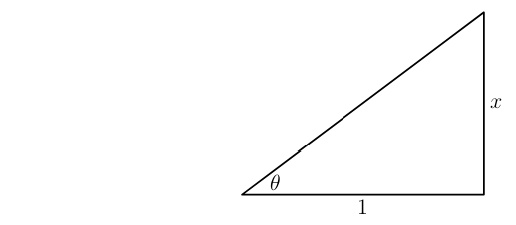
\includegraphics[width=6cm]{Capture44}\\
\centering
\text{\textbf{Figure:} Undoing trig substitution}
\end{figure}\\
This gives us $1/\sin\theta=\csc\theta=\sqrt{1+x^2}/x$ and
\begin{equation*}
\int\frac{1}{x^2\sqrt{1+x^2}}dx=-\frac{\sqrt{1+x^2}}{x}+c
\end{equation*}
(next page)
\newpage
\noindent\textbf{Example: Polar Coordinates}\\
Consider a circle of radius $a$, cut out a tab of height $b$:
\begin{figure}[h]
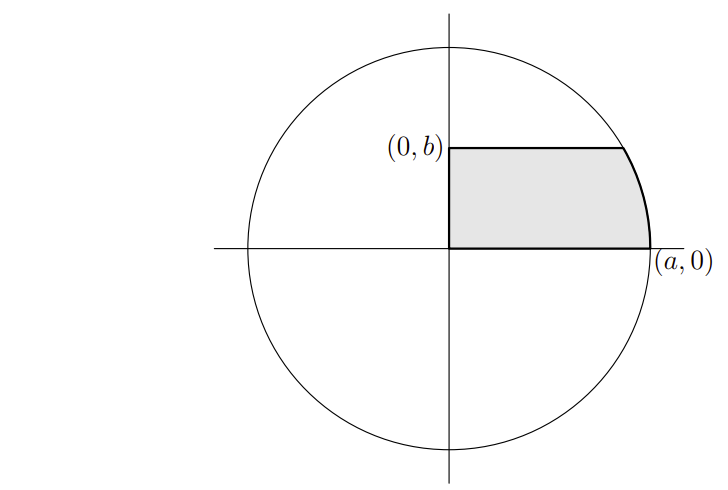
\includegraphics[width=6cm]{Capture42}\\
\centering
\text{\textbf{Figure:} Notice the upper border is non-differentiable} 
\end{figure}\\
An intuitive approach might be to integrate with respect to $y$, where the circle equation 
in terms of $x$ would be $x=\sqrt{a^2-y^2}$:
\begin{equation*}
\text{Area}=\int_0^bx\,dy=\int_0^b\sqrt{a^2-y^2}\,dy
\end{equation*}
One way to integrate this is by utilising polar coordinates:
\begin{figure}[h]
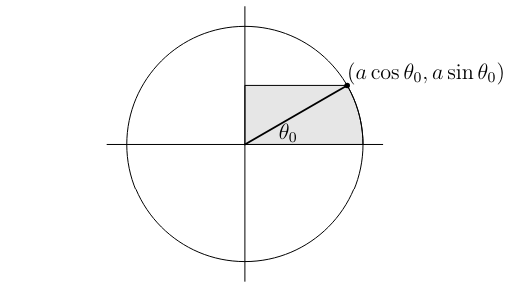
\includegraphics[width=8cm]{Capture43}\\
\centering
\text{\textbf{Figure:} Expression in terms of trigonometric functions} 
\end{figure}\\
We can express the coordinates of the upper right corner in terms of \textit{polar coordinates} 
$(a\cos\theta_0,a\sin\theta_0)$ (this is true in general).\\
(next page)
\newpage
\noindent Given our integral
\begin{equation*}
\text{Area}=\int_0^b\sqrt{a^2-y^2}\,dy
\end{equation*}
First consider the \textit{indefinite integral};
we substitute $y=a\sin\theta$ and\\ $dy=a\cos\theta\,d\theta$:
\begin{align*}
\int\sqrt{a^2-y^2}\,dy&=\int x\,dy\\
&=\int(a\cos\theta)(a\cos\theta)d\theta\\
&=a^2\int\cos^2x\,d\theta\\
&=a^2\left(\frac{\theta}{2}+\frac{\sin(2\theta)}{4}\right)+c
\end{align*}
We want to express our equation back in terms of $y$:
\begin{align*}
\int\sqrt{a^2-y^2}\,dy&=a^2\left(\frac{\theta}{2}+\frac{\sin(2\theta)}{4}\right)+c\\
&=a^2\left(\frac{\theta}{2}+\frac{\sin\theta\cos\theta}{2}\right)+c\\
&=\frac{a^2\theta}{2}+\frac{a\sin\theta\,a\cos\theta}{2}+c
\end{align*}
using $y=a\sin\theta$, we substitute
\begin{equation*}
\theta=\arcsin\left(\frac{y}{a}\right)
\end{equation*}
To get
\begin{equation*}
\int\sqrt{a^2-y^2}\,dy=\frac{a^2\arcsin(y/a)}{2}+\frac{y\sqrt{a^2-y^2}}{2}+c
\end{equation*}
Our definite integral, and therefore area, is given by
\begin{align*}
\int_0^b\sqrt{a^2-y^2}\,dy
&=\left.\left(\frac{a^2\arcsin(y/a)}{2}+\frac{y\sqrt{a^2-y^2}}{2}\right)\right|^b_0\\
&=\left(\frac{a^2\arcsin(b/a)}{2}+\frac{b\sqrt{a^2-b^2}}{2}\right)-0\\
&=\frac{a^2\arcsin(b/a)}{2}+\frac{b\sqrt{a^2-b^2}}{2}
\end{align*}
\newpage

\subsection{Summary of Trigonometric Substitution} %150624 {center}, {tabular}
Here are three basic forms which are integrated by trig substitution summarised
\begin{center}
\begin{tabular}{c|c|c}
Form&Substitute&Result\\[0.5ex]
\hline
&&\\
$\sqrt{a^2-x^2}$&$x=a\cos\theta$ or $x=a\sin\theta$&$a\sin\theta$ or $a\cos\theta$\\[2ex]
$\sqrt{a^2+x^2}$&$x=a\tan\theta$&$a\sec\theta$\\[2ex]
$\sqrt{x^2-a^2}$&$x=a\sec\theta$&$a\tan\theta$
\end{tabular}
\end{center}
Ugly integrals expressed in such a form are candidates for these methods.

\subsection{Partial Fractions}
Partial fractions allow for integration of functions of the form
\begin{equation*}
\frac{P(x)}{Q(x)}
\end{equation*}
Where $P(x)$ and $Q(x)$ are polynomials. Functions of this type are called \textit{rational functions}.
The method of partial fractions works by algebraically splitting $P(x)/Q(x)$ into pieces that
are easier to integrate. Consider
\begin{equation*}
\frac{4x-1}{(x-1)(x+2)}=\frac{A}{x-1}+\frac{B}{x+2}
\end{equation*}
We can solve for $A$ by:
\begin{align*}
\frac{4x-1}{(x-1)(x+2)}&=\frac{A}{x-1}+\frac{B}{x+2}\\
\frac{4x-1}{x+2}&=A+\frac{B}{x+2}(x-1)
\end{align*}
And substituting $x=1$ to get
\begin{equation*}
\frac{4(3)-1}{1+2}=A
\end{equation*}
(next page)
\newpage
\noindent\textbf{Repeated factors}\\
When faced with repeated factors in the denominator such as:
\begin{equation*}
\frac{x^2+2}{(x-1)^2(x+2)}
\end{equation*}
We require the addition of a second term for the repeated factor:
\begin{equation*}
\frac{x^2+2}{(x-1)^2(x+2)}=\frac{A}{x-1}+\frac{B}{(x-1)^2}+\frac{C}{x+2}
\end{equation*}
The same applies for factors repeated more times. Intuitively, this is the same as:
\begin{equation*}
\frac{7}{16}=\frac{0}{2}+\frac{1}{2^2}+\frac{1}{2^3}+\frac{1}{2^4}
\end{equation*}
\textbf{Quadratic Factors}\\
Consider
\begin{equation*}
\frac{x^2}{(x-1)(x^2+1)}
\end{equation*}
Notice the denominator cannot be split into any further factors
(other than using imaginary numbers). In this case we split the
fraction as follows:
\begin{equation*}
\frac{x^2}{(x-1)(x^2+1)}=\frac{A}{x-1}+\frac{Bx+C}{x^2+1}
\end{equation*}
The point here is that the numerator corresponding to the quadratic factor is linear, not
constant; generally it will be a polynomial with a degree one less than that of the denominator.
\newpage

\subsection{Integration by Parts} %170624
Integration of parts can be seen as the reverse of the product rule:
\begin{equation*}
(uv)'=u'v+uv'
\end{equation*}
We derive the formula for integration by parts from the product rule:
\begin{align*}
(uv)'&=u'v+uv'\\
uv'&=(uv)'-u'v\\
\int uv'dx&=\int(uv)'dx-\int u'v\,dx\\
\int uv'dx&=uv-\int u'v\,dx
\end{align*}
In the case of definite integrals:
\begin{equation*}
\int_a^buv'dx=uv|_a^b-\int_a^bu'v\,dx
\end{equation*}
\textbf{Example: }$\int\ln x\,dx$\\
Where $u=\ln x$, $v=1$, we get:
\begin{equation*}
\int\underbrace{\ln x}_{uv'}\,dx=\underbrace{(\ln x)(x)}_{uv}
-\int\underbrace{(\frac{1}{x})(x)}_{u'v}\,dx
\end{equation*}
and therefore
\begin{equation*}
\int\ln x\,dx=x\ln x-x+c
\end{equation*}
(next page)
\newpage
\noindent\textbf{Reduction Formulas}\\
Occasionally, integrals can be solved using \textit{reduction formulas}, where we apply a rule
to rewrite an integral in terms of another, simpler, integral.
Here are some examples:\\
\vspace{1mm}\\
\textbf{Example: }$\int(\ln x)^ndx$\\
Integrating by parts:
\begin{align*}
\int(\ln x)^ndx&=x(\ln x)^n-n\int(\ln x)^{n-1}\frac{1}{x}\cdot x\,dx\\
&=x(\ln x)^n-n\int(\ln x)^{n-1}\,dx
\end{align*}
Therefore, 
\begin{equation*}
F_n(x)=x(\ln x)^n-nF_{n-1}(x)\quad\text{where }F_i=\int(\ln x)^{i}dx
\end{equation*}
\textbf{Example: }$\int x^ne^xdx$
Replacing $e^x$ by $\sin x$ or $\cos x$ also leads to a similar derivation:
\begin{equation*}
\int x^ne^xdx=x^ne^x-\int nx^{n-1}e^xdx
\end{equation*}
where we get
\begin{equation*}
F_n(x)=x^ne^x-nF_{n-1}(x)\quad\text{where }F_i=\int x^ie^xdx
\end{equation*}
\newpage

\subsection{Arc length} %170624
Arc length can be calculated with a cumulative sum. Consider:
\begin{figure}[h]
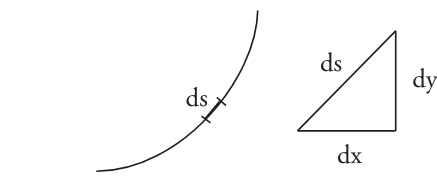
\includegraphics[width=8cm]{Capture45}\\
\centering
\text{\textbf{Figure:} Straight line approximation of arc length}
\end{figure}\\
We can approximate
\begin{equation*}
(\Delta s)^2\approx(\Delta x)^2+(\Delta y)^2
\end{equation*}
To get (as $\Delta s\to0$)
\begin{equation*}
ds=\sqrt{dx^2+dy^2}
\end{equation*}
We can factor out $dx$ to get
\begin{equation*}
\frac{ds}{dx}=\sqrt{1+\left(\frac{dy}{dx}\right)^2}
\end{equation*}
Therefore, if we have the $x$-coordinate range over our desired arc length:
\begin{align*}
\text{Arc Length}&=\text{Distance along the curve from $s_a$ to $s_b$}\\
&=\int_a^b\sqrt{1+\left(\frac{dy}{dx}\right)^2}dx=\int ds\\
&=\int_a^b\sqrt{1+f'(x)^2}dx
\end{align*}
Note that we are summing up changes in $s$, and not $y$. Thus we find arc length, not the area under the function.\\
(next page)
\newpage
\noindent\textbf{Example: Circular Arc}\\
Consider finding the arc length of a circle (centered at origin and radius 1), on 
the interval $0\leq x\leq a$:
\begin{figure}[h]
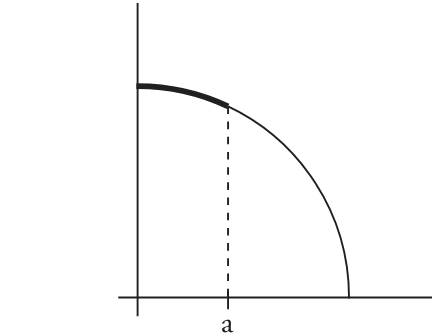
\includegraphics[width=6cm]{Capture46}\\
\centering
\text{\textbf{Figure:} Arc length of circle over $0\leq x\leq a$}
\end{figure}\\
Given our arc length formula, we need to find $f'(x)$:
\begin{align*}
y&=\sqrt{1-x^2}\\
y'&=\frac{-x}{\sqrt{1-x^2}}\\
\frac{ds}{dx}&=\sqrt{1+(y')^2}\\
&=\sqrt{1+\left(\frac{-x}{\sqrt{1-x^2}}\right)^2}
\end{align*}
We can simplify $1+\left(\frac{-x}{\sqrt{1-x^2}}\right)^2$:
\begin{align*}
\left(\frac{-x}{\sqrt{1-x^2}}\right)^2
&=1+\frac{x^2}{1-x^2}\\
&=\frac{1}{1-x^2}
\end{align*}
to get
\begin{equation*}
\frac{ds}{dx}=\sqrt{\frac{1}{1-x^2}}
\end{equation*}
(next page)
\newpage
\noindent Our arc length, $\alpha$, is therefore given by
\begin{align*}
\alpha&=\int_0^a\sqrt{\frac{1}{1-x^2}}dx\\
&=\left.\sin^{-1}x\right|_0^a\quad\text{(see \ref{fundamentals:differentiation:arcsin})}\\
\alpha&=\sin^{-1}a\quad\text{and}\quad\sin\alpha=a
\end{align*}
Notice that when our radius is 1, \textbf{the angle in radians is equal to our arc length}
\begin{figure}[h]
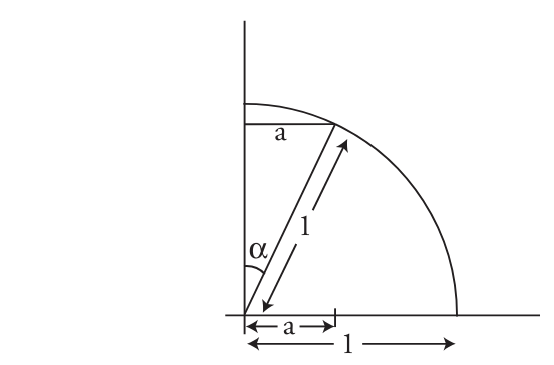
\includegraphics[width=6cm]{Capture47}\\
\centering
\text{\textbf{Figure:} angle (in radians) = arc length = $\alpha$}
\end{figure}\\
\vspace{1mm}
\newpage

\subsection{Parametric Equations} %170624
Parametric curves are essentially curves described by $x$ and $y$ being a function of a third 
variable $t$
\begin{align*}
x=x(t)\\
y=y(t)
\end{align*}
For instance, 
\begin{align*}
x=a\cos t\\
y=a\sin t
\end{align*}
Describes a circle:
\begin{align*}
x^2+y^2&=(x(t))^2+(y(t))^2\\
&=a^2\cos^2t+a^2\sin^2t\\
x^2+y^2&=a^2
\end{align*}
\begin{figure}[h]
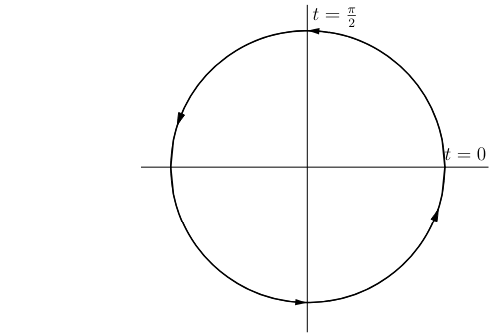
\includegraphics[width=6cm]{Capture48}\\
\centering
\text{\textbf{Figure:} $(a\cos t,a\sin t)$}
\end{figure}\\
\textbf{Example: Arc length}
Consider computing the arc length of the path of this trajectory. We have
\begin{align*}
ds&=\sqrt{dx^2+dy^2}\\
\frac{ds}{dt}&=\frac{1}{dt}\sqrt{dx^2+dy^2}\\
ds&=\sqrt{\left(\frac{dx}{dt}\right)^2+\left(\frac{dy}{dt}\right)^2}dt\\
\end{align*}
(next page)
\newpage
\noindent since
\begin{align*}
x&=a\cos t,\quad\frac{dx}{dt}=-a\sin t\\
y&=a\sin t,\quad\frac{dy}{dt}=-a\cos t
\end{align*}
We have
\begin{align*}
ds&=\sqrt{(-a\sin t)^2+(a\cos t)^2}dt\\
&=\sqrt{a^2}dt\\
&=a\,dt
\end{align*}
Should we define $t$ as time, we can conclude that a point moves
around the circle at speed $\frac{ds}{dt}=a$, constant speed.
\newpage

\subsection{Polar coordinates} %180624
Polar coordinates are another way of describing points in a plane:
\begin{figure}[h]
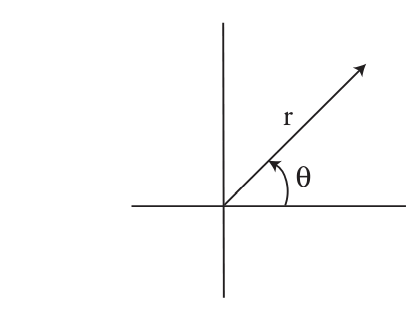
\includegraphics[width=6cm]{Capture49}\\
\centering
\text{\textbf{Figure:} Polar coordinates describe a radius $r$ and angle $\theta$}
\end{figure}\\
Unlike $x,y$ coordinates (called the rectangular coordinate system), which are essentially
coordinates on a grid,
Polar coordinates are defined by an angle and a distance to theorigin
Intuitively, therefore, conversion from polar coordinates to rectangular coordinates goes like
\begin{equation*}
x=r\cos\theta,\quad y=r\sin\theta
\end{equation*}
also intuitively, conversion from rectangular coordinates to polar coordinates:
\begin{equation*}
r=\sqrt{x^2+y^2},\quad\theta=\tan^{-1}\left(\frac{y}{x}\right)
\end{equation*}
Note this statement has ambiguity---$r$ could be $-\sqrt{x^2+y^2}$ and $\theta$ could be 
$\tan^{-1}\left(\frac{-y}{-x}\right)$. A diagramatic understanding of the coordinate is therefore also
required. Understand that 
both coordinate systems describe the \textit{same} space, just in different manners:
\begin{figure}[h]
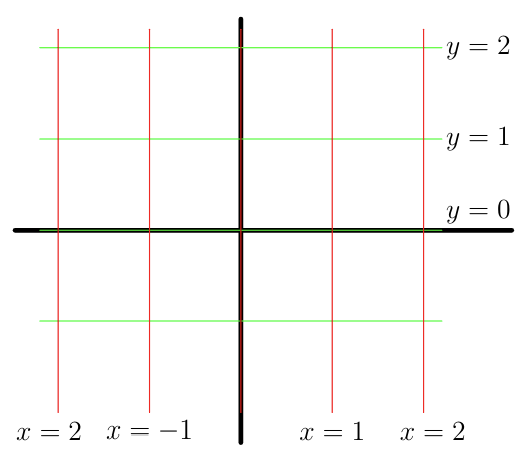
\includegraphics[width=5cm]{Capture50}
\includegraphics[width=5cm]{Capture51}\\
\centering
\text{\textbf{Figures:} Rectangular (left) vs Polar (right) coordinate systems}
\end{figure}\\
(next page)
\newpage
\noindent\textbf{Example: Translation into Polar Coordinates}\\
Consider translating $y=1$ into polar coordinates:
\begin{align*}
y&=r\sin\theta\\
1&=r\sin\theta\\
r&=\frac{1}{\sin\theta}
\end{align*}
Illustrated:
\begin{figure}[h]
\includegraphics[width=9cm]{Capture52}\\
\centering
\text{\textbf{Figure:} $r=\frac{1}{\sin\theta}$}
\end{figure}\\
Note here that as $\theta$ approaches 0 or $\pi/2$, $r$ tends to infinity. This gives us our
final answer:
\begin{equation*}
r=\frac{1}{\sin\theta},\quad0\leq\theta\leq\pi
\end{equation*}
\newpage

\subsection{Polar Coordinates and Area} %180624
We can directly calculate an area using polar coordinates. Similar to using Riemann sums, we 
divide the curve into 'slices':
\begin{figure}[h]
\includegraphics[width=7cm]{Capture53}\\
\centering
\text{\textbf{Figure:} A slice---radius $r$ and angle $d\theta$}
\end{figure}\\
where we can approximate each slice as a circular arc of arc length $rd\theta$. We define the 
incremental area of each slice as $dA$. To find $dA$, we use the idea that the proportion
of arc length is equal to the proportion of total area covered:
\begin{align*}
\frac{dA}{\pi r^2}&=\frac{rd\theta}{2\pi r}\\
dA&=\frac{d\theta}{2\pi }\cdot\pi r^2\\
dA&=\frac{1}{2}r^2d\theta
\end{align*}
Our final expression therefore looks like
\begin{equation*}
A=\int_{\theta_1}^{\theta_2}\frac{1}{2}r^2d\theta
\end{equation*}
Geometrically this looks like
\begin{figure}[h]
\includegraphics[width=8cm]{Capture54}\\
\centering
\text{\textbf{Figure:} Cumulative sum of area in 'slices' from curve to origin}
\end{figure}
\newpage

%%%%%%%%%%%%%%%%%%%%%%%%%%%%%%%%%%%%%%%%%%%%%%%%%%%%%%%%%%
%% L'Hospital's Rule, Improper Integrals, Taylor series %%
%%%%%%%%%%%%%%%%%%%%%%%%%%%%%%%%%%%%%%%%%%%%%%%%%%%%%%%%%%

\section{L'Hospital's Rule, Improper Integrals,\\ Taylor Series} %180624

\subsection{L'Hospital's Rule} %180624
L'Hospital's rule provides a systematic way of finding limits. Consider'the limit
\begin{equation*}
\lim_{x\to a}\frac{f(x)}{g(x)}
\end{equation*}
L'Hospital's rule states that if $\lim_{x\to c}f(x)=\lim_{x\to c}g(x)=0$ or $\pm\infty$, and $g'(x)\neq0$, then 
\begin{equation*}
\lim_{x\to c}\frac{f(x)}{g(x)}=\lim_{x\to c}\frac{f'(x)}{g'(x)}
\end{equation*}
\textbf{Intuition:}\\
Consider
\begin{equation*}
\lim_{x\to a}\frac{f(x)}{g(x)}
\end{equation*}
where the limit is indeterminate, for instance $f(a)=g(a)=0$. We can show
\begin{align*}
\lim_{x\to a}\frac{f(x)}{g(x)}
&=\lim_{x\to a}\frac{f(x)/(x-a)}{g(x)/(x-a)}\\
&=\frac{\lim_{x\to a}\frac{f(x)-f(a)}{x-a}}{\lim_{x\to a}\frac{g(x)-g(a)}{x-a}}
\quad(\text{since }f(a)=g(a)=0)\\
&=\frac{f'(a)}{g'(a)}\quad(\text{thus }g'(x)\neq0)
\end{align*}
\textbf{Example:}\\
Consider
\begin{equation*}
\lim_{x\to0}\frac{\sin5x}{\sin2x}
\end{equation*}
Since $a=0$, $f(a)=g(a)=0$, we apply L'Hospital's rule:
\begin{align*}
\lim_{x\to0}\frac{\sin5x}{\sin2x}&=\lim_{x\to0}\frac{5\cos5x}{2\cos2x}\\
&=\frac{5\cos(0)}{2\cos(0)}\\
&=\frac{5}{2}
\end{align*}
(next page)
\newpage
\noindent\textbf{Repeating L'Hospital's Rule}\\
If
\begin{equation*}
\lim_{x\to0}\frac{f'(x)}{g'(x)} 
\end{equation*}
is still indeterminate, L'Hospital's rule (if applicable) can be repeatedly used until a value 
is obtained. For instance, consider
\begin{equation*}
\lim_{x\to0}\frac{\cos x-1}{x^2}
\end{equation*}
Since $f(a)=g(a)=0$, we can apply L'Hospital's rule; notice however that the result is still indeterminate:
\begin{equation*}
\lim_{x\to0}\frac{\cos x-1}{x^2}=\lim_{x\to0}\frac{-\sin x}{2x}
\end{equation*}
Since $f'(a)=g'(a)=0$, we can apply L'Hospital's rule again:
\begin{align*}
\lim_{x\to0}\frac{\cos x-1}{x^2}
&=\lim_{x\to0}\frac{-\sin x}{2x}\quad\text{(L'Hop)}\\
&=\lim_{x\to0}\frac{-\cos x}{2}\quad\text{(L'Hop)}\\
&=\frac{-\cos0}{2}\\
&=-\frac{1}{2}
\end{align*}
Note that we only know that the hypotheses of L'Hospital's rule hold after we compute the 
limit---the theorem states that L'Hospital's rule only works if the limit exists.\\
\vspace{1mm}\\
\textbf{L'Hospital's rule extended:}\\
Note that L'Hospital's rule also works for
\begin{itemize}
\item $a=\pm\infty$
\item $f(a),g(a)=\pm\infty$
\item $\lim_{x\to a}\frac{f'(a)}{g'(a)}=\pm\infty$
\end{itemize}
Essentially it works for the $\frac{\infty}{\infty}$ case as well.
\newpage

\subsection{Examples of L'Hospital's Rule} %180624
\textbf{Example: }$\lim_{x\to0^+}x\ln x$\\
Notice we are multiplying a number that's getting smaller by one that's getting larger and 
larger; the result therefore depends on the rates of growth of each component.
\begin{equation*}
\lim_{x\to0^+}\underbrace{x}_{\to0}\underbrace{\ln x}_{\to-\infty}
\end{equation*}
We can rewrite the expression to apply L'Hospital's rule:
\begin{align*}
\lim_{x\to0^+}x\ln x&=\lim_{x\to0^+}\frac{\ln x}{1/x}\\
&=\lim_{x\to0^+}\frac{1/x}{-1/x^2}\quad\text{(L'Hop)}\\
&=\lim_{x\to0^+}-x\\
&=0
\end{align*}
Intuitively this means $x$ goes to 0 faster than $\ln x$ goes to $-\infty$, which may not have been apparent.\\
\vspace{1mm}\\
\textbf{Example: }$\lim_{x\to0+}x^x$\\
We can rewrite:
\begin{equation*}
x^x=e^{x\ln x}
\end{equation*}
to get
\begin{align*}
\lim_{x\to0+}x^x&=\lim_{x\to0+}e^{x\ln x}\\
&=e^{\lim_{x\to0+}x\ln x}\\
&=e^0\\
&=1
\end{align*}
Whenever applying L'Hospital's rule, one has to verify that \textit{they have an indeterminate form} 
for the rule to be valid.
\newpage

\subsection{L'Hospital's rule for rates of Growth and Decay} %180624
We can apply L'Hospital's rule to compare the rate at which functions change:\\
\vspace{1mm}\\
\textbf{Rates of Growth}\\
If $f(x)>0$ and $g(x)>0$ as $x$ approaches infinty, then
\begin{equation*}
f(x)<<g(x)\text{ as }x\to\infty\quad\text{means}\quad\lim_{x\to\infty}\frac{f(x)}{g(x)}=0
\end{equation*}
For instance, since
\begin{align*}
\lim_{x\to\infty}\frac{\ln x}{x^2}
&=\lim_{x\to\infty}\frac{1/x}{2x}\quad\text{(L'Hop)}\\
&=\lim_{x\to\infty}\frac{1}{2x^2}\\
&=0
\end{align*}
we can conclude that $\ln x<<x^2$ as $x\to\infty$. Other examples include: If $p>0$ then
\begin{equation*}
\ln x<<x^p<<e^x<<e^{x^2}\text{ as }x\to\infty
\end{equation*}
\textbf{Rates of Decay}
Similarly, we can compare rates at which functions tend to 0 as $x\to\infty$. If $p>0$ then
\begin{equation*}
\frac{1}{\ln x}>>\frac{1}{x^p}>>e^{-x}>>e^{-x^2}\text{ as }x\to\infty
\end{equation*}
\newpage

\subsection{Improper Integrals} %180624
\textit{Improper integrals} are definite integrals where one (or both) of the boundaries is 
at infinity, or where the integrand has a vertical asymptote in the interval of integration.
A possible improper integral of a function $f(x)>0$ is
\begin{equation*}
\int_a^\infty f(x)dx
\end{equation*}
which can also be written as a limit:
\begin{equation*}
\lim_{N\to\infty}\int_a^Nf(x)dx
\end{equation*}
The improper integral \textit{converges} if this limit exists and \textit{diverges} otherwise. 
Intutively, the geometric interpretation of the improper integral is the area under the curve
stretching to infinity; if the integral converges the defined area under the curve is finite;
otherwise it's infinite.\\
\vspace{1mm}\\
\textbf{Example: }$\int_1^\infty\frac{1}{x}dx$\\
We simply evaluate the integral (we let $N=\infty$ afterward):
\begin{align*}
\int_1^N\frac{1}{x}dx&=\ln x|^\infty_1\\
&=\ln(N)-\ln1\\
&=\ln(N)\to\infty\text{ as }N\to\infty
\end{align*}
This isn't quite intuitive, but we conclude that 
\begin{equation*}
\int_1^N\frac{1}{x}dx\text{ diverges}
\end{equation*}
It turns out that although $1/x$ diverges, $1/x^2$ \textit{converges}. This is not intuitively 
visible, necessitating methods to determine convergence.
\newpage

\subsection{Integral Comparison} %180624
During situations where we can't directly compute the area, we can use Integral/Limit 
Comparison to compare that function to another whose value we can compute. This will allow
us to tell us whether the former function converges or diverges\\
\vspace{1mm}\\
Consider that if $f(x)\sim g(x)$ as $x\to\infty$, then
$\int_a^\infty f(x)\,dx$ and $\int_a^\infty g(x)\,dx$ either both converge or both diverge.
($f(x)\sim g(x)$ as $x\to\infty$ means $\frac{f(x)}{g(x)}\to1$ as $x\to\infty$)\\
\vspace{1mm}\\
If we are unable to directly compute the integral of $g(x)$ to determine its convergence, 
we can instead compute that of $f(x)$, which converges in the same manner as $g$, in order
to circumvent the original problem.\\
\vspace{1mm}\\
\textbf{Example: }Use limit comparison to show $\int^\infty_1\frac{1}{(5x+2)^2}dx$ converges\\
We require a function $f(x)$ comparable to our given function $g(x)=\frac{1}{(5x+2)^2}$. 
One approach is to expand the denominator and discard its lower degree terms, giving us 
$g(x)=\frac{1}{25x^2}$. First we check that $f(x)\sim g(x)$:
\begin{align*}
\lim_{x\to\infty}\frac{f(x)}{g(x)}
&=\lim_{x\to\infty}\frac{\frac{1}{25x^2}}{\frac{1}{(5x+2)^2}}\\
&=\lim_{x\to\infty}\frac{25x^2+20x+4}{25x^2}\\
&=\lim_{x\to\infty}\left(1+\frac{4}{5x}
+\frac{4}{25x^2}\right)\\
\lim_{x\to\infty}\frac{f(x)}{g(x)}&=1
\end{align*}
Since $g(x)$ only converges if $f(x)$ does, we only need to determine the simple integral
\begin{align*}
\int_1^\infty\frac{1}{25x^2}dx&=\frac{1}{25}\int_1^\infty x^{-2}dx\\
&=\frac{1}{25}\left[-x^{-1}\right]_1^\infty\\
\int_1^\infty\frac{1}{25x^2}dx&=\frac{1}{25}
\end{align*}
We conclude that
\begin{equation*}
\int^\infty_1\frac{1}{(5x+2)^2}dx
\end{equation*}
must converge because
\begin{equation*}
\int^\infty_1\frac{1}{25x^2}dx
\end{equation*}
converges
\newpage

\subsection{Improper Integrals and Singularities} %200624
Here we consider integration near singular points. Integrals like these with discontinuities 
in the interval of integration are considered \textit{indefinite integrals of the second type}.
Examples include:
\begin{equation*}
\int_0^1\frac{dx}{\sqrt{x}},\quad\int_0^1\frac{dx}{x}\quad,
\int_0^1\frac{dx}{x^2}
\end{equation*}
These integrals turn out to be fairly straightforward to calculate:
\begin{align*}
\int_0^1\frac{dx}{\sqrt{x}}&=\int_0^1x^{-1/2}dx\\
&=\left.\frac{1}{1/2}x^{1/2}\right|_0^1\\
&=2
\end{align*}
\begin{align*}
\int_0^1\frac{dx}{x}&=\left.\ln x\right|_0^1\\
&=\ln1-\ln0\quad\text{(diverges)}
\end{align*}
\begin{align*}
\int_0^1\frac{dx}{x^2}&=\left.-x^{-1}\right|_0^1\\
&=-1+\left(\frac{1}{0}\right)\quad\text{(diverges)}
\end{align*}
(Notice how although the three functions intuitively have a similar shape, one of them 
converges while the others diverge)\\
\vspace{1mm}\\
Note that we have to be careful near singularities---integrating over the singularity will
lead to a nonsensical answer:
\begin{equation*}
\int_{-1}^1\frac{dx}{x^2}=-2\quad\text{despite }\frac{1}{x^2}>0
\end{equation*}
Fact is that the area here is infinite, not -2\\
(next page)
\newpage
\noindent\textbf{Improper Integrals of the Second Kind}\\
Similar to other improper integrals, we can express integrals near singularities as limits; 
consider $f(x)=\frac{1}{x}$, which has a singularity at 0:
\begin{equation*}
\int_0^1f(x)\,dx=\lim_{a\to0^+}\int_a^1f(x)\,dx
\end{equation*}
As before, we say the integral \textit{converges} if this limit exists and \textit{diverges} 
if not:
\begin{figure}[h]
\includegraphics[width=6cm]{Capture55}\\
\centering
\text{\textbf{Figure:} Area under the graph of 
$y=\frac{1}{x}$} 
\end{figure}\\
In general, regarding the singularity near 0 for $\frac{1}{x^p}$:
\begin{align*}
\int_0^1\frac{1}{x^p}&=\left.\frac{x^{-p+1}}{-p+1}\right|_0^1\quad\text{(for $p\neq1$)}\\
&=\frac{1^{-p+1}}{-p+1}-\frac{0^{-p+1}}{-p+1}\\
&=
\begin{cases}
\frac{1}{-p+1}\quad&\text{if }p<1\\
\text{diverges}\quad&\text{if }p\geq1
\end{cases}
\end{align*}
(next page)
\newpage
\noindent\textbf{Some intuition}\\
Despite being of a similar shape, the limits of $\int\frac{1}{x^p}$ differ depending on $p$.
Here we propose an intuitive understanding; calculating limits, we find
\begin{align*}
\frac{1}{x^{-1/2}}<<\underbrace{\frac{1}{x}<<\frac{1}{x^2}}_{\text{diverges}}\quad\text{as }
x\to0^+\\
\underbrace{\frac{1}{x^{-1/2}}>>\frac{1}{x}}_{\text{diverges}}>>\frac{1}{x^2}\quad\text{as }
x\to\infty
\end{align*}
The idea is that $\frac{1}{x}$ is symmetric to itself by a reflection across the line $y=x$, 
and the areas under the curve for $x\geq1$ and $0\leq x\leq1$ are both $\infty$.
\begin{figure}[h]
\includegraphics[width=6cm]{Capture56}\\
\centering
\text{\textbf{Figure:} Area under the graph of 
$y=\frac{1}{x}$ is infinite in both directions} 
\end{figure}\\
Now consider the $\frac{1}{x^{1/2}}$; it isn't symmetric about $y=x$, and one 'tail' larger
than the other:
\begin{figure}[h]
\includegraphics[width=5cm]{Capture57}
\includegraphics[width=5cm]{Capture58}\\
\centering
\text{\textbf{Left figure:} Area under the graph of 
$y=\frac{1}{x^{1/2}}$ is infinite in only one direction}\\
\text{\textbf{Right figure:} $\frac{1}{x}$ superimposed onto
$\frac{1}{x^{1/2}}$}
\end{figure}\\
Notice the difference when $\frac{1}{x}$ is superimposed onto
$\frac{1}{x^{1/2}}$; comparing the 'tails' of the functions allows for a geometric sense
of the difference between convergent and divergent integrals.\\
(next page)
\newpage
\noindent Comparing the tails of $\frac{1}{x^2}$ and $\frac{1}{x}$, we see that the divergent nature of 
the 'tails' can also be seen here:
\begin{figure}[h]
\includegraphics[width=5cm]{Capture59}
\includegraphics[width=5cm]{Capture60}\\
\centering
\text{\textbf{Left figure:} Area under the graph of 
$y=\frac{1}{x^{2}}$ is infinite in only one direction}\\
\text{\textbf{Right figure:} $\frac{1}{x}$ superimposed onto
$\frac{1}{x^{2}}$}
\end{figure}
\newpage

%%%%%%%%%%%%%%%%%%%%%%%%%%% 
%% limits and continuity %% 
%%%%%%%%%%%%%%%%%%%%%%%%%%%

\section{Limits and Continuity} %140524
\label{fundamentals:limits and continuity}

\subsection{Limits} %140524 {cases}
\label{fundamentals:limits and continuity:limits}
Limits can be further subdivided into right and left-handed limits. The limit:
\begin{equation*}
\lim_{x\to x_0^+}f(x)
\end{equation*}
Is called a \textit{right-hand limit}, meaning values to the right of $x_0$ on the number
line should be used to compute the limit. For instance consider $f(x)$:
\begin{align*}
f(x)=
\begin{cases} 
x+1 &\quad x \geq 0 \\
-x  &\quad x < 0
\end{cases}
\end{align*}
\begin{figure}[h]
\includegraphics[width=9cm]{Capture3}
\centering
\end{figure}\\
In this case the right-hand limit $\lim_{x\to 0^+}f(x)$ is 1. Similarly, the 
\textit{left-hand limit}:
\begin{equation*}
\lim_{x\to x_0^-}f(x)
\end{equation*} 
is found when values to the \textit{left} of $x_0$ on the number line
are used to compute the limit. In this case, $\lim_{x\to 0^-}f(x)=0$.

\newpage
\subsection{Continuity and Differentiability} %140524 {itemize}, \item
\textbf{Definition:} A function is \textit{continuous} at $x_0$ if $\lim_{x\to x_0}f(x)=f(x_0)$.\\
More specifically, a function continuous at $x_0$ has the properties:
\begin{itemize}
\item $\lim_{x\to 0^+}f(x)=\lim_{x\to 0^-}f(x)$; and both of these one sided limits exist. 
\item $f(x_0)$ is defined.
\item $\lim_{x\to 0^+}f(x)=\lim_{x\to 0^-}f(x)=f(x_0)$.
\end{itemize}
Remember that when calculating $\lim_{x\to x_0}f(x)$ one never allows
$x$ to equal $x_0$. Note that $\lim_{x\to x_0}f(x)$ is calculated differently and independently
of $f(x_0)$; if one isn't careful to make this distinction, this definition has no meaning.\\
\vspace{2mm}\\
The same concept applies to \textbf{differentiability}, where a function is
\textit{differentiable} at $x_0$ if $\lim_{x\to x_0}f'(x)=f'(x_0)$, and:
\begin{itemize}
\item $\lim_{x\to 0^+}f'(x)=\lim_{x\to 0^-}f'(x)$; and both of these one sided limits exist. 
\item $f'(x_0)$ is defined.
\item $\lim_{x\to 0^+}f'(x)=\lim_{x\to 0^-}f'(x)=f'(x_0)$.
\end{itemize}

\subsection{Discontinuity} %140524
A non-continuous function implies the presence of a \textit{discontinuity}. Here are a few
types of discontinuities:\\
A \textbf{Jump Discontinuity} occurs when the right and left-hand limits exist but are not equal,
the example in \ref{fundamentals:limits and continuity:limits} is an instance of this:
\begin{figure}[h]
\includegraphics[width=9cm]{Capture3}
\centering
\end{figure}\\
Although $\lim_{x\to 0^+}f(x)$ and $\lim_{x\to 0^-}f(x)$ exist, they are \textbf{not equal};
therefore this function is discontinuous.
\newpage
\noindent A \textbf{Removable Discontinuity} occurs when the right and left-hand limits are equal but either
the function is not defined or not equal to these limits:
\begin{equation*}
\lim_{x\to 0^+}f(x)=\lim_{x\to 0^-}f(x)\neq f(x_0)
\end{equation*}
\begin{figure}[h]
\includegraphics[width=9cm]{Capture4}
\centering
\text{\textbf{Figure:} A removable discontinuity, continuous everywhere except one point.}
\end{figure}\\
An example of this is...%TBC REFER TO NOTESa
\\
\vspace{2mm}\\
In an \textbf{Infinite discontinuity}, the left and right-hand limits are infinite,
either limit may be negative or positive:
\begin{figure}[h]
\includegraphics[width=9cm]{Capture5}
\centering
\text{\textbf{Figure:} An infinite discontinuity: $\frac{1}{x}$}
\end{figure}\\
In this case, $\lim_{x\to 0^+}f(x)=\infty$, while $\lim_{x\to 0^-}f(x)=-\infty$ note that a limit 
of $\infty$ is different from saying a limit doesn't exist.
\newpage

\subsection{Differentiable implies Continuous} %140524
\textbf{Theorem:} If $f$ is differentiable at $x_0$, then $f$ is continuous at $x_0$.\\
\textbf{Proof:} We need to show
\begin{align*}
&\lim_{x\to x_0}f(x)=f(x_0)\\
&\lim_{x\to x_0}f(x)-f(x_0)=0
\end{align*}
We can prove this through:
\begin{equation*}
\lim_{x\to x_0}f(x)-f(x_0)=\lim_{x\to x_0}\frac{f(x)-f(x_0)}{x-x_0}(x-x_0)
\end{equation*}
Notice that when $x\to x_0$, we can say
\begin{equation*}
\lim_{x\to x_0}f(x)=\lim_{\Delta x\to 0}f(x_0+\Delta x)
\end{equation*}
and that 
\begin{equation*}
\lim_{x\to x_0}x=\lim_{\Delta x\to 0}(x_0+\Delta x)
\end{equation*}
going back to the original equation:
\begin{align*}
\lim_{x\to x_0}\frac{f(x)-f(x_0)}{x-x_0}(x-x_0)
&=\lim_{\Delta x\to 0}\frac{f(x_0+\Delta x)-f(x_0)}{(x_0+\Delta x)-x_0}((x_0+\Delta x)-x_0)\\
&=\lim_{\Delta x\to 0}\frac{f(x_0+\Delta x)-f(x_0)}{\Delta x}(\Delta x)
\end{align*}
Now assuming that $f$ is \textbf{differentiable} at $x_0$:
\begin{align*}
\lim_{x\to x_0}f(x)-f(x_0)&=\lim_{x\to x_0}\frac{f(x)-f(x_0)}{x-x_0}(x-x_0)\\
&=\lim_{\Delta x\to 0}\frac{f(x_0+\Delta x)-f(x_0)}{\Delta x}(\Delta x)\\
&=f'(x)\cdot 0\\
&=0
\end{align*}
Notice that our assumption that $f$ was differentiable at $x_0$ leads to\\ 
$\lim_{x\to x_0}f(x)-f(x_0)=0$, indicating that differentiability implies continuity.\\
Also note that dividing by $\lim_{x\to x_0}(x-x_0)$ is not the same as division by 0 since 
$\lim_{x\to x_0}(x-x_0)$ never truly reaches 0.
\vspace{2mm}\\
(Note that one might intuively understand that $\lim_{x\to x_0}\frac{f(x)-f(x_0)}{x-x_0}=f'(x)$
in line 6. I've changed the limit to produce the difference quotient for ease of understanding.)
\newpage

\section{Infinite Series} %200624

\subsection{Notation} %200624
We define a \textit{partial sum} to be 
\begin{equation*}
S_N=\sum^N_{n=0}a_n
\end{equation*}
Similar to indefinite integrals, we can define
\begin{equation*}
S=\sum^\infty_{n=0}a_n=\lim_{N\to\infty}S_N
\end{equation*}
Where if the limit exists the series \textit{converges}, and otherwise \textit{diverges}.

\subsection{Integral Comparison for Series} %200624
Evaluating the limits of series is tends to be difficult. Integral comparison allows us
to understand series limits in terms of integrals:\\
\vspace{1mm}\\
\textbf{Theorem} If $f(x)$ is decreasing and $f(x)>0$ on the interval $[1,\infty]$, then
the sum $\sum^\infty_1f(n)$ and the integral $\int_1^\infty f(x)\,dx$ diverge and converge together and
\begin{equation*}
\sum^\infty_1f(n)-\int_1^\infty f(x)\,dx<f(1)
\end{equation*}
\textbf{Example:} Do the series $\sum^\infty_{n=2}\frac{1}{n\ln n}$ and 
$\sum^\infty_{n=2}\frac{1}{n(\ln n)^2}$ converge or diverge?\\
\vspace{1mm}\\
First we should check that the functions of interest are decreasing and positive on the specified interval. 
Then with the Integral comparison test we can say that since
\begin{align*}
\int_2^\infty\frac{1}{x\ln x}dx=\infty\quad\text{diverges}\\
\sum^\infty_{n=2}\frac{1}{n\ln n}\quad\text{diverges}
\end{align*}
and that since
\begin{align*}
\int_2^\infty\frac{1}{x(\ln x)^2}dx=\ln2\quad\text{converges}\\
\sum^\infty_{n=2}\frac{1}{n(\ln n)^2}\quad\text{converges}
\end{align*}
(next page)
\newpage
\noindent\textbf{Intuition for Integral comparison: Harmonic Series}\\
Consider comparing:
\begin{equation*}
\sum^\infty_{n=1}\frac{1}{n}\quad\text{with}\quad\int_1^\infty\frac{dx}{x}
\end{equation*}
Notice that the summation is just an upper Riemann sum of the integral with $\Delta x=1$:
\begin{figure}[h]
\includegraphics[width=6cm]{Capture61}\\
\centering
\text{\textbf{Figure:} The summation \textit{is} an upper Riemann sum of the function}
\end{figure}\\
Intuitively we can see that the upper Riemann sum is greater than the integral:
\begin{equation*}
\int^N_1\frac{dx}{x}<1+\frac{1}{2}+\frac{1}{3}+\ldots+\frac{1}{N-1}
\end{equation*}
(There are $N-1$ rectangles because the distance between 1 and $N$ is $N-1$.) If $S_N=1+\frac{1}{2}+\frac{1}{3}+\ldots+\frac{1}{N}$, we can further say
\begin{equation*}
\int^N_1\frac{dx}{x}<1+\frac{1}{2}+\frac{1}{3}+\ldots+\frac{1}{N-1}<S_N
\end{equation*}
This allows us to conclusively prove that the series diverges:
\begin{equation*}
\int^N_1\frac{dx}{x}=\ln N<S_N
\end{equation*}
Since $\lim_{N\to\infty}\ln N=\infty$.\\
(next page)
\newpage
\noindent Since for $f(x)=\frac{1}{x}$, $\ln N<S_N$ and $\ln N$ diverges, 
\begin{equation*}
\lim_{N\to\infty}S_N=\sum_{n=1}^\infty\frac{1}{n}\quad\text{diverges}
\end{equation*}
Now consider the lower Riemann sum:
\begin{figure}[h]
\includegraphics[width=6cm]{Capture62}\\
\centering
\text{\textbf{Figure:} Lower Riemann sum of $\frac{1}{x}$}
\end{figure}\\
Intuitively we see that
\begin{align*}
\int^N_1\frac{dx}{x}&>\frac{1}{2}+\frac{1}{3}+\ldots+\frac{1}{N}=S_N-f(1)\\
\ln N&>S_N-f(1)\\
\ln N+f(1)&>S_N
\end{align*}
Combining this with the result from the upper Riemann sum we can conclude
\begin{align*}
\int^N_1\frac{dx}{x}=\ln N&<S_N<\ln N+f(1)=\int^N_1\frac{dx}{x}+f(1)\\
\int^N_1\frac{dx}{x}&<\sum_{n=1}^N\frac{1}{n}<\int^N_1\frac{dx}{x}+f(1)\\
&\left|\sum_{n=1}^N\frac{1}{n}-\int^N_1\frac{dx}{x}\right|<f(1)
\end{align*}
\newpage

\subsection{Limit Comparison for Series} %210624
Similar to with integrals, Limit comparison can be used with two series to determine convergence properties:\\
\vspace{1mm}\\
\textbf{Theorem}: If $f(n)\sim g(n)$ (i.e if $\lim_{n\to\infty}\frac{f(n)}{g(n)}=1$) and 
$g(n)>0$ for all $n$, then $\sum^\infty_{n=1}f(n)$ and $\sum^\infty_{n=1}g(n)$ converge or diverge together.\\
\vspace{1mm}\\
\textbf{Example}: Does $\sum_{n=0}^\infty\frac{5n+2}{n^3+1}$ converge or diverge?\\
We can compare 
\begin{equation*}
\sum_{n=0}^\infty\frac{5n+2}{n^3+1}\quad\text{with}\quad\sum_{n=1}^\infty\frac{5n}{n^3}
=\sum_{n=1}^\infty\frac{5}{n^2}
\end{equation*}
We should check the $f(n)\sim g(n)$:
\begin{align*}
\lim_{n\to\infty}\frac{f(n)}{g(n)}&=\lim_{n\to\infty}\frac{\frac{5n+2}{n^3+1}}{\frac{5}{n^2}}\\
&=\lim_{n\to\infty}\frac{5n^3+2n^2}{5n^3+5}=1
\end{align*}
Thus since $\sum_{n=1}^\infty\frac{5}{n^2}$ converges, 
$\sum_{n=0}^\infty\frac{5n+2}{n^3+1}$ also converges.
\newpage

\subsection{Ratio Test for convergence of series} %210624
A ratio text can be used to determine the convergence properties of a series. Say we have
a series
\begin{equation*}
\sum a_n\quad\text{where $a_n>0$}
\end{equation*}
Now consider the limit:
\begin{equation*}
\lim_{n\to\infty}\frac{a_{n+1}}{a_n}=L
\end{equation*}
We can say that if
\begin{align*}
L<1,&\quad\sum a_n\text{ converges}\\
L>1,&\quad\sum a_n\text{ diverges}
\end{align*}
(For $L=1$ different cases can occur and we can't make any deductions)\\
\vspace{1mm}\\
\textbf{Intuition}\\
Consider the case where
\begin{equation*}
\lim_{n\to\infty}\frac{a_{n+1}}{a_n}=L<1
\end{equation*}
We can say for some large $n>n_0$ ($n_0$ just defines some threshold for $n$)
\begin{equation*}
\frac{a_{n+1}}{a_n}<r=\frac{r^{n+1}}{r^n}
\end{equation*}
$r$ is a ratio with value $L<r<1$. Since the limit of $\frac{a_{n+1}}{a_n}$ tends to $L$, we can say that for some high enough $n$ 
eventually this criteria is met. With that we get
\begin{align*}
\frac{a_{n+1}}{a_n}&<\frac{r^{n+1}}{r^n}\\
\frac{a_{n+1}}{r^{n+1}}&<\frac{a_n}{r^n}
\end{align*}
Note the meaning of this: the ratio between $a_n$ and $r^n$ is decreasing.
Therefore for large enough $n$:
\begin{equation*}
a_n<kr^n
\end{equation*}
(remember this isn't necessarily true all the way throughout the series), but now we can say
\begin{equation*}
\sum_{n=n_0}a_n<k\sum_{n=n_0}r^n
\end{equation*}
since we defined $r$ to be $L<r<1$, $k\sum_{n=n_0}r^n$ converges, and therefore so does
$\sum_{n=n_0}a_n$. This means that 
\begin{equation*}
\sum a_n\quad\text{converges}
\end{equation*}
(next page)
\newpage
\noindent\textbf{Example:} Does $\sum\frac{4^n}{n3^n}$ converge or diverge?
\begin{align*}
\lim_{n\to\infty}\frac{a^{n+1}}{a_n}&=\lim_{n\to\infty}\frac{4^{n+1}}{(n+1)3^{n+1}}\cdot
\frac{n3^n}{4^n}\\
&=\lim_{n\to\infty}\frac{4n}{3(n+1)}\\
&=\frac{4}{3}>1\quad\text{(diverges)}
\end{align*}
\textbf{Example:} Does $\sum\frac{n^10}{10^n}$ converge or diverge?
\begin{align*}
\lim_{n\to\infty}\frac{(n+1)^{10}}{10^{n+1}}\cdot\frac{n^{10}}{10^n}
&=\lim_{n\to\infty}\frac{1}{10}\cdot\frac{(n+1)^{10}}{n^{10}}\\
&=\frac{1}{10}<1\quad\text{(converges)}
\end{align*}
\newpage

\subsection{Power Series} %210624
\textbf{General Power Series and Radius of Convergence:}\\
In general, a power series is of the form 
\begin{equation*}
a_0+a_1x+a_2x^2+a_3x^3+\ldots=\sum^\infty_{n=0}a_nx^n
\end{equation*}
A power series converges when $-R<x<R$, where $R$ is called the \textit{radius of convergence}; the value of $R$ depends on the coefficients $a_i$. 
When $|x|>R$, the series diverges; correspondingly when $|x|<R$, the series converges.\\
\vspace{1mm}\\
When $|x|<R$, the values of each term in the series will tend to 0 exponentially fast. While in the $|x|>R$ case the values won't tend to 0 at all.\\
\vspace{1mm}\\
\textbf{Example:} 
Consider the power series with the sum:
\begin{equation*}
1+x+x^2+x^3+\ldots=\frac{1}{1-x}\quad(|x|<1)
\end{equation*}
We prove the sum here; denoting $S$ to be the sum:
\begin{align*}
1+x+x^2+x^3+\ldots&=S\\
x+x^2+x^3+x^4+\ldots&=Sx\\
1+0+0+\ldots&=S-Sx
\end{align*}
(Note that $Sx$ contains one more higher degree $x$ than $S$, but since high degree terms tend to 0 (since $S$ converges as it tends to a constant), 
that higher degree term tends to 0.)
\begin{align*}
1&=S-Sx\\
S&=\frac{1}{1-x}
\end{align*}
If it wasn't obvious already, $S$ has to converge in order for it to exist; this leads to the requirement for $|x|<1$---the radius
of convergence in this case is 1.\\
(next page)
\newpage
\noindent\textbf{Ratio Test to find Radius of Convergence}\\
One can apply a ratio test to find the radius of convergence. For a series
$\sum_{n=n_0}^\infty c_nx^n$ we can apply the ratio test to find
\begin{equation*}
L=\lim_{n\to\infty}\left|\frac{c_{n+1}x^{n+1}}{c_{n}x^{n}}\right|
\end{equation*}
(Note the ratio test still intuitively makes sense even when taking the absolute value of the limit.) Point here is that we are able 
to find the value of $x$ for which $L$ crosses 1---meaning the point where the series stops converging and starts diverging,
giving us the radius of convergence.\\
\vspace{1mm}\\
\textbf{Example:} Radius of Convergence of $\sum_{n=1}^\infty\frac{x^n}{n}$\\
In this case
\begin{align*}
\frac{c_{n+1}x^{n+1}}{c_{n}x^{n}}&=\frac{x^{n+1}/(n+1)}{x^n/n}\\
&=x\cdot\frac{n}{n+1}
\end{align*}
and so our ratio test gives us
\begin{align*}
L&=\lim_{n\to\infty}\left|\frac{c_{n+1}x^{n+1}}{c_{n}x^{n}}\right|\\
&=\lim_{n\to\infty}\left|x\cdot\frac{n}{n+1}\right|\\
&=\lim_{n\to\infty}\left|x\cdot\left(1-\frac{1}{n+1}\right)\right|\\
L&=|x|
\end{align*}
When $|x|<1,L<1$ and the series will converge. When $|x|>1,L>1$ and the series diverges---the radius of convergence is 1.
\newpage

\subsection{Taylor's Series} %220624
\textbf{Taylor's formula}\\
The formula is given as
\begin{equation*}
f(x)=\sum^\infty_{n=0}\frac{f^{(n)}(0)}{n!}x^n
\end{equation*}
\textbf{Intuition}\\
Consider
\begin{align*}
f(x)&=a_0+a_1x+a_2x^2+a_3x^3+\ldots\\
f'(x)&=a_1+2a_2x+3a_3x^2+\ldots\\
f''(x)&=(1\cdot2)a_2+(2\cdot3)a_3x+(3\cdot4)a_4x^2+\ldots\\
f^{(3)}(x)&=(1\cdot2\cdot3)a_3+(2\cdot3\cdot4)a_4x+\ldots
\end{align*}
Notice that by substituting in $x=0$, 
\begin{equation*}
f^{(n)}(0)=(n!)a_n
\end{equation*}
Thus
\begin{equation*}
a_n=\frac{f^{(n)}(0)}{n!}
\end{equation*}
\textbf{Examples}\\
Using this procedure we can evaluate:
\begin{align*}
e^x&=\sum^{\infty}_{n=0}\frac{1}{n!}x^n\\
\sin x&=x-\frac{x^3}{3!}+\frac{x^5}{5!}-\frac{x^7}{7!}+\ldots\\
\cos x&=1-\frac{x^2}{2!}+\frac{x^4}{4!}-\frac{x^6}{6!}+\ldots
\end{align*}
\textbf{More intuition:}\\
Note that a more general form of the Taylor expansion can also be considered:
\begin{equation*}
f(x)=\sum_{n=0}^\infty\frac{f^{(n)}(c)}{n!}(x-c)^n
\end{equation*}
(expansion at $x=c$ instead of 0)
A finite Taylor series expansion is simply a $n$-degree approximation at a specific point (think of it as being similar to Fourier series!).
Note that although an 'infinite' expansion should equal the function of interest, it is the \textit{limit} of the series that approaches 
the function---we won't ever have a 'closed form expression' using these expansions. 
\newpage

\subsection{When a function is equivalent to its Taylor series} %230624
We address the question of when a function is equal to its Taylor Series. Recall that
a series can be expressed as limits:
\begin{equation*}
\sum_{n=0}^\infty a_n=\lim_{N\to\infty}\sum^N_{n=0}a_n
\end{equation*}
In the context of Taylor series $T_f(x)$ for a function $f$, the Taylor series can be expressed as the limit of 
a limit of Taylor Polynomials $P_N(x)$ as $N\to\infty$:
\begin{equation*}
T_f(x)=\sum_{n=0}^\infty\frac{f^{(n)}(x)}{n!}(x-c)^n
=\lim_{N\to\infty}\sum^N_{n=0}\frac{f^{(n)}(x)}{n!}(x-c)^n=\lim_{N\to\infty}P_N(x)
\end{equation*}
Where $P_N(x)$ is the $N$-th degree Taylor polynomial to $f(x)$ at $x=c$.
Notice $f(x)$ will equal $T_f(x)$ provided
\begin{equation*}
f(x)-\lim_{N\to\infty}P_N(x)=\lim_{N\to\infty}(f(x)-P_N(x))=0
\end{equation*}
We can denote $f(x)-P_N(x)$ to be the 'remainder' $R_N(x)$. A function therefore equals its Taylor series when 
\begin{equation*}
\lim_{N\to\infty}R_N(x)=0
\end{equation*}
To proceed we use Taylor's inequality.\\
\vspace{1mm}\\
\textbf{Taylor's inequality.} \textit{If $f(x)$ is $n$-times differentiable and $|f^{(n)}(x)|\leq M$ for all $x\in[c,c+d]$, then}
\begin{equation*}
|f(x)-P_{n-1}(x)|\leq\frac{M}{n!}(x-c)^n
\end{equation*}
Intuition: (base case $n=1$) If $f^{(1)}\leq M$ for $x\in[c,c+d]$,
\begin{align*}
\int_c^xf^{(1)}(t)dt&\leq\int_c^xM\,dt\\
f(x)-f(c)&\leq M(x-c)\\
f(x)&\leq f(c)+M(x-c)\\
&=P_0(x)+\frac{M}{1!}(x-c)^1
\end{align*}
(proof can be carried out by induction)\\
(next page)
\newpage
\noindent Returning to the original problem, taylor's inequality gives us\\
\vspace{1mm}\\
If $f(x)$ is $(n+1)$-times differentiable and $|f^{(n+1)}(x)|\leq M$ for all $x\in[c-d,c+d]$, then
\begin{align*}
|f(x)-P_N(x)|=|R_N(x)|\leq\frac{M}{(N+1)!}|x-c|^{N+1}
\end{align*}
For all $x\in[c-d,c+d]$.\\
\vspace{1mm}\\ 
\textbf{Show thet $e^x$ converges to its Taylor Series} at 0 for all real $x$:\\
We first find some $M$ where $|f^{(n+1)}(x)|\leq M$ for all $x\in[c-d,c+d]$; knowing that the derivative of $e^x$ is itself, an increasing function,
and that we are interested in convergence to the taylor series near 0, a suitable bound would be:
\begin{equation*}
|f^{(N+1)}(x)|\leq e^d\quad\text{for all $x$ in $[-d,d]$}
\end{equation*}
Using $e^d$ in our inequality:
\begin{align*}
\lim_{N\to\infty}|R_N(x)|&\leq\lim_{N\to\infty}\frac{e^d}{(N+1)!}|x|^{N+1}\\
&=\lim_{N\to\infty}e^d\frac{|x|^{N+1}}{(N+1)!}\\
&=0
\end{align*}
\newpage

%%%%%%%%%%%%%%%%%%%%%%%%%%%%
%% Differential Equations %%
%%%%%%%%%%%%%%%%%%%%%%%%%%%%
\section{Differential Equations}

\subsection{Introduction to Ordinary Differential Equations\\(ODEs)} %030624
Here we introduce intuition for  Ordinary Differential Equations (ODEs) and introductory solving methods.\\
\vspace{1mm}\\
The simplest type of differential equation looks like:
\begin{equation*}
\frac{dy}{dx}=f(x)
\end{equation*}
which can be solved by the antiderivative $y=\int f(x)\,dx$. \\
\vspace{1mm}\\
\textbf{Intuition}\\
Now we consider a more interesting example: 
\begin{equation*}
\frac{dy}{dx}+xy=0
\end{equation*}
This equation can be solved by \textit{separation of variables}:
\begin{align*}
\frac{dy}{dx}+xy&=0\\
\frac{dy}{dx}&=-xy\\
\frac{dy}{y}&=-x\,dx
\end{align*}
Since the problem is now set up in terms of differentials rather than ratios of differentials,
we can integrate both sides.
\begin{align*}
\int\frac{dy}{y}&=-\int x\,dx\\
\ln y+c_1&=-\frac{x^2}{2}+c_2\quad\text{(assume $y>0$)}
\end{align*}
We can combine the constants and simplify:
\begin{align*}
\ln y&=-\frac{x^2}{2}+c\\
e^{\ln y}&=e^{-x^2/2+c}\\
y&=e^ce^{-x^2/2}\\
y&=Ae^{-x^2/2},\quad\text{(where $A=e^c$})
\end{align*}
(The more apt $\ln|y|$ simplifies to $\pm Ae^{-x^2/2}$, which doesn't matter since $A$ is some
unspecific constant)\\
(next page)
\newpage
\noindent It turns out that our solution,
\begin{equation*}
y=Ae^{-x^2/2},\quad\text{(where $A=e^c$})
\end{equation*}
Works for any constant multiple $A$. We can check this 
solution:
\begin{align*}
y&=ae^{-x^2/2}\\
\frac{dy}{dx}&=\frac{d}{dx}ae^{-x^2/2}\\
&=a\cdot(-x)e^{-x^2/2}\\
&=-x\cdot ae^{-x^2/2}\\
\frac{dy}{dx}&=-xy
\end{align*}
$A$ is determined by an initial condition; for instance if $y(0)=1$, $A=1$.
\newpage

\subsection{Separation of Variables} %030524
Here we describe a rudimentary method for solving some differential equations---\\Separation of Variables.\\
\vspace{1mm}\\
In general, this method applies to differential equations of the form
\begin{equation*}
\frac{dy}{dx}=f(x)g(y)
\end{equation*}
Where we then \textit{separate} the variables and integrate:
\begin{align*}
\frac{dy}{dx}&=f(x)g(y)\\
\frac{dy}{g(y)}&=f(x)\,dx\\
h(y)\,dy&=f(x)\,dx\quad\text{where }h(y)=\frac{1}{g(y)}\\
\int h(y)\,dy&=\int f(x)\,dx\\
\end{align*}
Antidifferentiating both sides:
\begin{equation*}
H(y)=\int h(y)\,dy;\quad F(x)=\int f(x)\,dx
\end{equation*}
we now have
\begin{align*}
H(y)+c_1&=F(x)+c_2\\
H(y)&=F(x)+c
\end{align*}

%%%%%%%%%%%%%%%%%%%%%%%%%
%%%%%%%%%%%%%%%%%%%%%%%%%
%%%%%%%%%%%%%%%%%%%%%%%%%

\chapter{Multivariable Calculus/Calculus III}

\section{Vectors and Matrices} %250624 \langle\rangle
\subsection{Notation, Terminology}
For reference regarding notation for vectors and matrices:
\begin{figure}[h]
\includegraphics[width=6cm]{Capture63}\\
\centering
\end{figure}\\
We regard $\mathbf{A}$ as an \textit{origin vector}, written as
\begin{equation*}
\mathbf{A}=\langle a_1,a_2\rangle
\end{equation*}
Vectors $\mathbf{i}$ and $\mathbf{j}$ denote \textit{unit vectors} (vectors of magnitude 1) $\mathbf{i}=
\langle 1,0\rangle$, $\mathbf{j}=\langle 0,1\rangle$.
As such,
\begin{equation*}
\langle a_1,a_2\rangle=a_1\mathbf{i}+a_2\mathbf{j}
\end{equation*}
(next page)
\newpage
\noindent\textbf{Vector algebra}\\
As illustrated,
\begin{figure}[h]
\includegraphics[width=10cm]{Capture64}\\
\centering
\end{figure}
\begin{itemize}
\item Addition: $\mathbf{A+B}=(a_1+b_1)\mathbf{i}+(a_2+b_2)\mathbf{j};\\
\langle a_1,a_2\rangle+\langle b_1,b_2\rangle=
\langle a_1+b_1,a_2+b_2\rangle$
\item Subtraction: $\mathbf{A-B}=(a_1-b_1)\mathbf{i}+(a_2-b_2)\mathbf{j};\\
\langle a_1,a_2\rangle-\langle b_1,b_2\rangle=
\langle a_1-b_1,a_2-b_2\rangle$
\item Magnitude: $\mathbf{|A|}=\sqrt{a_1^2+a_2^2}$ (Pythagorean theorem)
\end{itemize}
In three dimensions:
\begin{figure}[h]
\includegraphics[width=5cm]{Capture65}
\includegraphics[width=5cm]{Capture66}\\
\centering
\end{figure}\\
Similarly, we denote $\mathbf{A}=\langle a_1,a_2,a_3\rangle$, 
$\mathbf{i}=\langle 1,0,0\rangle$, $\mathbf{j}=\langle 0,1,0\rangle$, 
$\mathbf{k}=\langle 0,0,1\rangle$, where
\begin{equation*}
\langle a_1,a_2,a_3\rangle=a_1\mathbf{i}+a_2\mathbf{j}+a_3\mathbf{k}
\end{equation*}
Magnitude in three dimensions also follows from the Pythagorean theorem:
\begin{equation*}
|a_1\mathbf{i}+a_2\mathbf{j}+a_3\mathbf{k}|=|\langle a_1,a_2,a_3\rangle|
=\sqrt{a_1^2+a_2^2+a_3^2}
\end{equation*}
\newpage

\subsection{Proof for Law of cosines} %250624
\begin{figure}[h]
\includegraphics[width=8cm]{Capture67}\\
\centering
\end{figure}
\noindent We show
\begin{equation*}
c^2=a^2+b^2-2ab\cos C
\end{equation*}
Consider
\begin{align*}
CD&=a\cos C\\
DA&=b-a\cos C\quad(1)\\
BD&=a\sin C\quad(2)
\end{align*}
Using the pythagorean theorem:
\begin{align*}
c^2&=DA^2+BD^2\\
&=(b-a\cos C)^2+(a\sin C)^2\\
&=b^2-2ab\cos C+a^2(\sin^2C+\cos^2C)\\
c^2&=a^2+b^2-2ab\cos C
\end{align*}
\newpage

\subsection{Dot product} %250624
The dot product has Algebraic and Geometric perspectives:\\
\textit{Algebraic view} (for 2D vectors)\\
If $\mathbf{A}=\langle a_1,a_2\rangle$ and $\mathbf{B}=\langle b_1,b_2\rangle$ then
\begin{equation*}
\mathbf{A\cdot B}=a_1b_1+a_2b_2
\end{equation*}
\textit{Geometric view}\\
Given $\mathbf{A,B}$ with angle $\theta$ between them:
\begin{figure}[h]
\begin{equation*}
\mathbf{A\cdot B}=\mathbf{|A||B|}\cos\theta
\end{equation*}
\includegraphics[width=8cm]{Capture68}\\
\centering
\end{figure}\\
\textbf{Intuition}\\
We can use the law of cosines to show that the two views are the same:
\begin{equation*}
\mathbf{|A-B|^2=|A|^2+|B|^2}-2\mathbf{|A|B|\cos\theta}
\end{equation*}
given $\mathbf{A}=\langle a_1,a_2\rangle$ and $\mathbf{B}=\langle b_1,b_2\rangle$,
\begin{align*}
2\mathbf{|A|B|\cos\theta}&=\mathbf{|A|^2+|B|^2-|A-B|^2}\\
&=\left(\sqrt{a_1^2+a_2^2}\right)^2+\left(\sqrt{b_1^2+b_2^2}\right)^2-
\left(\sqrt{(a_1-b_1)^2+(a_2-b_2)^2}\right)^2\\
&=a_1^2+a_2^2+b_1^2+b_2^2-[(a_1-b_1)^2+(a_2-b_2)^2]\\
2\mathbf{|A|B|\cos\theta}&=2a_1b_1+2a_2b_2
\end{align*}
this simplifies to
\begin{align*}
a_1b_1+a_2b_2&=\mathbf{|A|B|\cos\theta}\\
\mathbf{A\cdot B}&=\mathbf{|A||B|}\cos\theta
\end{align*}
(next page)
\newpage
\noindent\textbf{Components and Projection}\\
If $\mathbf{A}$ is any vector and $\mathbf{\hat{u}}$ is a unit vector then the \textit{component}
of $\mathbf{A}$ in the direction of $\mathbf{\hat{u}}$ is 
\begin{equation*}
\mathbf{A\cdot\hat{u}}
\end{equation*}
(Note that the component is a scalar) This can be seen from:
\begin{equation*}
\mathbf{A\cdot\hat{u}=|A||\hat{u}|\cos\theta=|A|\cos\theta}\quad
\text{(since $\mathbf{\hat{u}}$ is a unit vector)}
\end{equation*}
Geometrically:
\begin{figure}[h]
\includegraphics[width=6cm]{Capture69}\\
\centering
\end{figure}\\
The dot product here is the \textit{orthogonal projection} of $\mathbf{A}$ on 
$\mathbf{\hat{u}}$. The concept of components also extends to non-unit vectors, where
the component of $\mathbf{A}$ in the direction of $\mathbf{B}$ is 
\begin{equation*}
\mathbf{A\cdot\left(\frac{B}{|B|}\right)}
\end{equation*}
(Essentially the dot product with the unit vector in the same direction as $\mathbf{B}$)\\
\vspace{1mm}\\
\textbf{Testing for orthogonality}\\
Since $\cos(\pi/2)=0$, the dot product gives a test for orthogonality between vectors:
\begin{equation*}
\mathbf{A\perp B}\iff\mathbf{A\cdot B}=0
\end{equation*}
\newpage

\subsection{Determinant---Intuition} %250624
Consider attempting to find the area of a triangle, where $\mathbf{A}=\langle a_1,a_2\rangle$ and $\mathbf{B}=\langle b_1,b_2\rangle$:
\begin{figure}[h]
\includegraphics[width=3cm]{Capture70}\\
\centering
\end{figure}\\
Intuitively,
\begin{align*}
\text{Area}&=\frac{1}{2}\cdot\text{Base}\cdot\text{Height}\\
&=\frac{1}{2}\mathbf{|A||B|\sin\theta}
\end{align*}
now consider an approach where we express this area as a dot product:
\begin{figure}[h]
\includegraphics[width=4cm]{Capture71}
\includegraphics[width=4cm]{Capture72}\\
\centering
\end{figure}\\
Rotating $\mathbf{A}$ by $\pi/2$, notice that
\begin{equation*}
\sin\theta=\cos\theta'\quad\text{(where $\theta'=\frac{\pi}{2}-\theta$)}
\end{equation*}
Since $\mathbf{|A'|=|A|}$, we get
\begin{align*}
\frac{1}{2}\mathbf{|A||B|\sin\theta}&=\frac{1}{2}\mathbf{|A'||B|\cos\theta'}\\
&=\frac{1}{2}(\mathbf{A'\cdot B})
\end{align*}
(next page)
\newpage
\noindent Notice our expression $(\mathbf{A'\cdot B})$ simplifies to
\begin{align*}
\mathbf{A'\cdot B}
&=\langle -a_2,a_1\rangle\cdot\langle b_1,b_2\rangle\\
&=a_1b_2-a_2b_1
\end{align*}
This absolute value of this result is double the area of our triangle, or the 
area of a parallelogram formed by $\mathbf{A}$ and $\mathbf{B}$:
\begin{figure}[h]
\includegraphics[width=3cm]{Capture70}
\includegraphics[width=7cm]{Capture73}\\
\centering
\end{figure}\\
This result is known as the \textit{determinant}:
\begin{align*}
\pm\text{area}(\diamond)&=\mathbf{|A||B|\sin\theta}\\
&=a_1b_2-a_2b_1\\
&=\det(\mathbf{A,B})\\
\pm\text{area}(\triangleleft)&=\frac{1}{2}\mathbf{|A||B|\sin\theta}\\
&=\frac{1}{2}\det(\mathbf{A,B})
\end{align*}
(Note that since $\sin\theta$ can be negative we take the absolute value of the
determinant to be the area)
\newpage

\subsection{Determinant---Definition} %260624
\textbf{2D determinant}
\begin{figure}[h]
\includegraphics[width=5cm]{Capture74}\\
\centering
\begin{align*}
\pm\det
\begin{pmatrix}
a_1 & a_2\\
b_1 & b_2
\end{pmatrix}
&=\pm
\begin{vmatrix}
a_1 & a_2\\
b_1 & b_2
\end{vmatrix}\\
&=\text{Area of parallelogram with edges $\mathbf{A}=(a_1,a_2)$, $\mathbf{B}=(b_1,b_2)$}\\
\end{align*}
\end{figure}\\
\textbf{3D determinant}
\begin{figure}[h]
\includegraphics[width=5cm]{Capture75}\\
\centering
\begin{align*}
\pm\det
\begin{pmatrix}
a_1 & a_2 & a_3\\
b_1 & b_2 & b_3\\
c_1 & c_2 & c_3
\end{pmatrix}
&=\pm
\begin{vmatrix}
a_1 & a_2 & a_3\\
b_1 & b_2 & b_3\\
c_1 & c_2 & c_3
\end{vmatrix}\\
&=\text{Area of parallelepiped with edges row vectors $\mathbf{A,B,C}$}.
\end{align*}
\end{figure}\\
Generalising, $n\times n$ determinants can be interpreted as the hypervolume 
in $n$-space of a $n$-dimensional parallelotope.
\newpage

\subsection{Computing Determinants}%260624
In the $2\times2$ case:
\begin{equation*}
\begin{vmatrix}
a & b\\
c & d
\end{vmatrix}
=ad-bc
\end{equation*}
Note that $\left|
\begin{smallmatrix}
a & c\\
b & d
\end{smallmatrix}\right|$ 
gives the same answer.\\
\vspace{1mm}\\
\textbf{$3\times3$ determinants}\\
We first define notation for matrix entries:
\begin{equation*}
\begin{vmatrix}
a_{11} & a_{12}\\
a_{21} & a_{22}
\end{vmatrix}\quad\quad
\begin{vmatrix}
a_{11} & a_{12} & a_{13}\\
a_{21} & a_{22} & a_{23}\\
a_{31} & a_{32} & a_{33}
\end{vmatrix}
\end{equation*}
\begin{itemize}
\item The \textbf{ij-entry}, written $a_{ij}$, is the number in the $i$-th row and $j$-th column.
\item The \textbf{ij-minor}, written $|A_{ij}|$, is the determinant that is left 
after deleting from $|A|$ the row and column containing $a_{ij}$.
\item The \textbf{ij-cofactor}, written $A_{ij}$, is given as a formula by 
$A_{ij}=(-1)^{i+j}|A_{ij}|$. Notice that in the case of the $3\times3$ determinant the
sign of the cofactor changes in a checkerboard pattern:
\begin{equation*}
\begin{vmatrix}
+ & - & +\\
- & + & -\\
+ & - & +
\end{vmatrix}
\end{equation*}
\end{itemize}
\textbf{Laplace expansion by cofactors} to evaluate a determinant in the $3\times3$ case occurs as follows: 
\textit{Select any row (or column) of the determinant. Multiply each entry $a_{ij}$ in that row (or column)
by its cofactor $A_{ij}$ and add the three resulting numbers to get the determinant}.\\
\vspace{1mm}\\
Therefore, Laplace expansion of a third order ($3\times3$) determinant using cofactors of the first row:
\begin{equation*}
a_{11}A_{11}+a_{12}A_{12}+a_{13}A_{13}=|A|
\end{equation*}
using cofactors in the $j$-th column:
\begin{equation*}
a_{1j}A_{1j}+a_{2j}A_{2j}+a_{3j}A_{3j}=|A|
\end{equation*}
\textbf{Example}
\begin{align*}
\begin{vmatrix}
a & b & c\\
d & e & f\\
g & h & i
\end{vmatrix}
&=a\cdot
\begin{vmatrix}
e & f\\
h & i
\end{vmatrix}
-b\cdot
\begin{vmatrix}
d & f\\
g & i
\end{vmatrix}
+c\cdot
\begin{vmatrix}
d & e\\
g & h
\end{vmatrix}\\
&=a(ei-fh)-b(di-fg)+c(dh-eg)
\end{align*}
(next page)
\newpage
\noindent\textbf{Larger determinants}\\
$n\times n$ determinants are evaluated in the same way; the Laplace expansion
in the $i$-th row would be
\begin{equation*}
|A|=a_{i1}A_{i1}+a_{i2}A_{i2}+\ldots+a_{in}A_{in}
\end{equation*}
Note that this is an inductive calculation---it expresses the determinant of order 
$n$ in terms of determinants of order $n-1$.\\
\vspace{1mm}\\
\textbf{Example} (Laplace expansion by first row)
\begin{align*}
&\begin{vmatrix}
a & b & c & d\\
e & f & g & h\\
i & j & k & l\\
m & n & o & p
\end{vmatrix}\\
=&a\cdot
\begin{vmatrix}
f & g & h\\
j & k & l\\
n & o & p
\end{vmatrix}
-b\cdot
\begin{vmatrix}
e & g & h\\
i & k & l\\
m & o & p
\end{vmatrix}
+c\cdot
\begin{vmatrix}
e & f & h\\
i & j & l\\
m & n & p
\end{vmatrix}
-d\cdot
\begin{vmatrix}
e & f & g\\
i & j & k\\
m & n & o
\end{vmatrix}\\
=&\ldots
\end{align*}
The Laplace expansion can be used as the basis of an inductive definition of the $n\times n$ determinant.\\
\vspace{1mm}\\
Note a few properties of $|A|$ ($A$ is a square array)
\begin{itemize}
\item $|A|$ is multiplied by -1 if we interchange two rows or two columns
\item $|A|=0$ if one row or column is all zero, or if two rows or two columns are the same
\item $|A|$ is multiplied by $c$ if every element of some row or column is multiplied by $c$.
\item The value of $|A|$ is unchanged if we add to one row (or column) a constant multiple of another row
\end{itemize}

\newpage

\subsection{Cross Product/Vector Product---Definition and formula} %260624
Here we describe algebraic and geometric perspectives of the cross product.\\
\textbf{Determinant definition for cross product}\\
Given vectors $\mathbf{A}=\langle a_1,a_2,a_3\rangle$ and $\mathbf{B}=\langle b_1,b_2,b_3\rangle$,
we define the cross product by
\begin{align*}
\mathbf{A\times B}&=
\begin{vmatrix}
\mathbf{i} & \mathbf{j} & \mathbf{k}\\
a_1 & a_2 & a_3\\
b_1 & b_2 & b_3
\end{vmatrix}\\
&=\mathbf{i}
\begin{vmatrix}
a_2 & a_3\\
b_2 & b_3
\end{vmatrix}
-\mathbf{j}
\begin{vmatrix}
a_1 & a_3\\
b_1 & b_3
\end{vmatrix}
+\mathbf{k}
\begin{vmatrix}
a_1 & a_2\\
b_1 & b_2
\end{vmatrix}\\
&=(a_2b_3-a_3b_2)\mathbf{i}+(a_3b_1-a_1b_3)\mathbf{j}
+(a_1b_2-a_2b_1)\mathbf{k}\\
&=\langle a_2b_3-a_3b_2,a_3b_1-a_1b_3,a_1b_2-a_2b_1\rangle 
\end{align*}
$\mathbf{i,j,k}$ are the unit vectors for the $x,y,z$ axes (Note that the top line 
is technically flawed since we aren't allowed to use vectors as entries in a determinant).\\
\textbf{Example}
\begin{equation*}
\mathbf{i\times j}=
\begin{vmatrix}
\mathbf{i} & \mathbf{j} & \mathbf{k}\\
1 & 0 & 0\\
0 & 1 & 0
\end{vmatrix}
=\mathbf{i}(0)-\mathbf{j}(0)+\mathbf{k}(1)=\mathbf{k}
\end{equation*}
\textbf{Geometric description}\\
The magnitude of $\mathbf{A\times B}$ is
\begin{align*}
|\mathbf{A\times B}|&=|\mathbf{A}||\mathbf{B}|\sin\theta\quad
(\theta\text{ being the angle between $\mathbf{A}$ and $\mathbf{B}$})\\
&=\text{Area of parallelogram spanned by $\mathbf{A}$ and $\mathbf{B}$}
\end{align*}
The direction of $\mathbf{A\times B}$ is perpendicular to the plane of $\mathbf{A}$ and $\mathbf{B}$. 
The directon is given by the \textit{right hand rule}---pointing one's fingers in the direction of 
$\mathbf{A}$ and curling them toward $\mathbf{B}$, one's thumb would point in the direction of 
$\mathbf{A\times B}$:
\begin{figure}[h]
\includegraphics[width=10cm]{Capture76}\\
\centering
\end{figure}\\
(next page)
\newpage
\noindent Note therefore, a few properties of the cross product:
\begin{itemize}
\item $\mathbf{A\times A=0}$
\item $\mathbf{A\times B=-B\times A}$ (Anti-commutivity)
\item $\mathbf{A\times(B+C)=A\times B+A\times C}$
(Distributive)
\item $\mathbf{(A\times B)\times C\neq A\times(B\times C)}$ (Non-associativity)
\end{itemize}
For the unit vectors $\mathbf{i,j,k}$, we have
\begin{equation*}
\mathbf{i\times j=k,\quad j\times k=i,\quad k\times i=j}
\end{equation*}

\newpage

\subsection{Equations of Planes I} %270624
\textbf{Intuition}\\
Consider a plane made up of three points $P_1,P_2,P_3$. 
We want to determine whether a point $P=(x,y,z)$ is in the plane:
\begin{figure}[h]
\includegraphics[width=6cm]{Capture77}\\
\centering
\end{figure}\\
One approach would be to compute the determinant of the three vectors formed by the four points;
since if $P$ were within the plane the volume of the parallelepiped formed by the
three points would be zero. Thus $P$ is within the plane if
\begin{equation*}
\det(\overrightarrow{\mathbf{P_1P_2}},\overrightarrow{\mathbf{P_1P_3}},\overrightarrow{\mathbf{P_1P}})=0
\end{equation*}
Another approach would be to find the \textit{normal vector} $\overrightarrow{\mathbf{N}}$ to the plane; 
where if $\overrightarrow{\mathbf{P_1P}}$ is orthogonal to $\overrightarrow{\mathbf{N}}$, then 
$P$ lies within the plane: 
\begin{figure}[h]
\includegraphics[width=6cm]{Capture78}\\
\centering
\end{figure}\\
We find $\overrightarrow{\mathbf{N}}$ using the cross product:
\begin{equation*}
\overrightarrow{\mathbf{N}}=\overrightarrow{\mathbf{P_1P_2}}\times\overrightarrow{\mathbf{P_1P_3}}
\end{equation*}
Orthogonality can then be tested using the dot product, giving us
\begin{equation*}
\overrightarrow{\mathbf{P_1P}}\cdot\overrightarrow{\mathbf{N}}=\overrightarrow{\mathbf{P_1P}}\cdot
(\overrightarrow{\mathbf{P_1P_2}}\times\overrightarrow{\mathbf{P_1P_3}})=0
\end{equation*}
if $P$ is within the plane. It turns out that this expression, called the \textit{triple product},
is equal to the determinant:
\begin{align*}
b\times c&=(b_2c_3-b_3c_2,b_3c_1-b_1c_3,b_1c_2-b_2c_1)\\
\underbrace{a\cdot(b\times c)}_{\text{triple product}}&=a_1b_2c_3-a_1b_3c_2+a_2b_3c_1-a_2b_1c_3+a_3b_1c_2-a_3b_2c_1\\
&=\det\left(
\begin{pmatrix}
a_1&b_1&c_1\\
a_2&b_2&c_2\\
a_3&b_3&c_3
\end{pmatrix}\right)\\
\end{align*}
(next page)
\newpage
\noindent\textbf{Example}\\
We can use this to find the equation of a plane. Consider a plane 
containing three points $P_1=(1,3,1), P_2=(1,2,2), P_3=(2,3,3)$. We have two vectors   
$\overrightarrow{\mathbf{P_1P_2}}$ and $\overrightarrow{\mathbf{P_1P_3}}$ in the plane, 
so we have 
\begin{equation*}
\overrightarrow{\mathbf{N}}=\overrightarrow{\mathbf{P_1P_2}}\times\overrightarrow{\mathbf{P_1P_3}}
=(-2,1,1)
\end{equation*}
Since for any point $P$ in the plane $\overrightarrow{\mathbf{P_1P}}$ is orthogonal to $\mathbf{N}$, we have
\begin{align*}
\overrightarrow{\mathbf{N}}\cdot\overrightarrow{\mathbf{P_1P}}&=0\\
(-2,1,1)\cdot(x-1,&y-3,z-1)=0\\
-2x+y+z&=2
\end{align*}
\newpage

\subsection{Matrix Operations}
\textbf{1. Scalar multiplication}\\
Multiplying each entry by a scalar
\begin{equation*}
cA=(ca_{ij})
\end{equation*}
\textbf{2. Matrix addition}\\
Addition of corresponding entries (as such both matrices have to be of the same size)
\begin{equation*}
A+B=(a_{ij}+b_{ij})
\end{equation*}
\textbf{3. Transposition}\\
The \textit{transpose} of the $m\times n$ matrix $A$ is the $n\times m$ matrix 
obtained by making the rows of $A$ the columns of the new matrix, denoted by $A^T$:
\begin{align*}
\text{If}\quad A&=
\begin{pmatrix}
a&b&c\\
d&e&f
\end{pmatrix}
,\quad A^T=
\begin{pmatrix}
a&d\\
b&e\\
c&f
\end{pmatrix}\\
\text{If}\quad A&=
\begin{pmatrix}
a&b\\
c&d
\end{pmatrix}
,\quad A^T=
\begin{pmatrix}
a&c\\
b&d
\end{pmatrix}
\end{align*}
\textbf{4. Matrix multiplication}\\
Schematically, we have
\begin{align*}
\underbrace{A}_{m\times n}\quad\cdot\quad\underbrace{B}_{n\times p}\quad
&=\quad\underbrace{C}_{m\times p}\\
\text{where}\quad c_{ij}=&\sum_{k=1}^na_{ik}b_{kj}
\end{align*}
For the multiplication to be defined, $A$ must have as many \textit{columns} as $B$ has \textit{rows}.
The $ij$-th entry of the product matrix $C$ is the dot product of the $i$-th row of $A$
with the $j$-th column of $B$.\\
(next page)
\newpage
\noindent\textbf{Properties of matrix multiplication}
\begin{itemize}
\item Distributive: $A(B+C)=AB+AC,\quad(A+B)C=AC+BC$
\item Associative: $(AB)C=A(BC)$
\item Given \textit{identity} matrix $I$, $AI=IA$
\item In general, $AB\neq BA$ (non-commutative). (There are some important exceptions, such as 
in the case with the identity matrix)
\item For two square $n\times n$ matrices $A$ and $B$. We have the \textit{determinant law}:
\begin{equation*}
|AB|=|A||B|\quad\text{or}\quad\det(AB)=\det(A)\det(B)
\end{equation*}
\end{itemize}
\textbf{Extraction of single row or column}
A useful fact is that a simple row or column vector can be used to pick out a row or column of 
a given matrix as follows:
\begin{align*}
\begin{pmatrix}
a & b & c\\
d & e & f\\
g & h & i
\end{pmatrix}
\begin{pmatrix}
0\\1\\0
\end{pmatrix}
&=
\begin{pmatrix}
b\\e\\h
\end{pmatrix}
\quad\text{(Middle column)}\\
\begin{pmatrix}
1&0&0
\end{pmatrix}
\begin{pmatrix}
a & b & c\\
d & e & f\\
g & h & i
\end{pmatrix}
&=
\begin{pmatrix}
a&b&c
\end{pmatrix}
\quad\text{(First row)}
\end{align*}
\newpage

\subsection{Meaning of Matrix Multiplication} %280624
\textbf{Matrices as transformations}\\
Given two matrices $A$ and $B$, $AB$ can be seen as 
representing:
\begin{equation*}
\text{\textit{Do transformation $B$, then transformation $A$}}
\end{equation*}
Matrix multiplication is done \textit{right to left}; with the first multiplication representing
a transformation from the basic unit vectors.\\
\textbf{Example}\\
The matrix $\left(\begin{smallmatrix}0&-1\\1&0\end{smallmatrix}\right)$ represents a 
plane rotation by $90^{\circ}$ counter clockwise;
consider how multiplication changes the unit vectors:
\begin{align*}
&\begin{bmatrix*}[r]
0&-1\\1&0
\end{bmatrix*}
\begin{bmatrix}
1\\0
\end{bmatrix}
=\begin{bmatrix}
0\\1
\end{bmatrix}\\
&\begin{bmatrix*}[r]
0&-1\\1&0
\end{bmatrix*}
\begin{bmatrix}
0\\1
\end{bmatrix}
=\begin{bmatrix*}[r]
-1\\0
\end{bmatrix*}
\end{align*}
Visualised:
\begin{figure}[h]
\includegraphics[width=5cm]{Capture79}\\
\centering
\begin{align*}
\begin{bmatrix*}[r]
0&-1\\1&0
\end{bmatrix*}
\begin{bmatrix*}[r]
x\\y
\end{bmatrix*}
=\begin{bmatrix*}[r]
-y\\x
\end{bmatrix*}
\end{align*}
\end{figure}\\
(next page)
\newpage
\noindent\textbf{More intuition about determinants}\\
The matrix $A=\left(\begin{smallmatrix}4&1\\1&3\end{smallmatrix}\right)$ 
transforms the unit square into a parallelogram as follows:
\begin{align*}
\begin{bmatrix*}[r]
4&1\\1&3
\end{bmatrix*}
\begin{bmatrix*}[r]
1\\0
\end{bmatrix*}
=\begin{bmatrix*}[r]
4\\1
\end{bmatrix*},\quad\quad
\begin{bmatrix*}[r]
4&1\\1&3
\end{bmatrix*}
\begin{bmatrix*}[r]
0\\1
\end{bmatrix*}
=\begin{bmatrix*}[r]
1\\3
\end{bmatrix*}
\end{align*}
Notice the transformation of the unit vectors leads to new vectors with endpoints
specified in $A$:
\begin{figure}[h]
\includegraphics[width=9cm]{Capture80}\\
\centering
\end{figure}\\
The resulting parallelogram has edges that are identical to the entries of $A$.\\
\vspace{1mm}\\
Notice that the area of this parallelogram can be found therefore using
\begin{equation*}
\text{Area of resulting parallelogram}=\det(A)
\end{equation*}
illustrating a relationship between a change in area after a transformation 
and the corresponting determinant. 
\newpage

\subsection{Matrix Inverses---Intuition} %290624
Consider a linear system of equations:
\begin{align*}
a_{11}x_1+a_{12}x_2+a_{13}x_3=b_1\\
a_{21}x_1+a_{22}x_2+a_{23}x_3=b_2\\
a_{31}x_1+a_{32}x_2+a_{33}x_3=b_3
\end{align*}
In such systems $a_{ij}$ and $b_i$ are given, and we want to solve for $x_i$. 
We can use matrix multiplication to abbreviate the system by
\begin{equation*}
A\mathbf{x=b},\quad
\mathbf{x}=
\begin{pmatrix}
x_1\\x_2\\x_3
\end{pmatrix},\quad
\mathbf{b}=
\begin{pmatrix}
b_1\\b_2\\b_3
\end{pmatrix}
\end{equation*}
Where $A$ is the square matrix of coefficients $(a_{ij})$. Notice that this works 
for any $n\times n$ system of equations. Given $\mathbf{b}$ and $A$, we want to solve for $\mathbf{x}$.\\
\vspace{1mm}\\
With that, suppose we could find a square matrix $M$, the same size as $A$, such that
\begin{equation*}
MA=I\quad\text{($I$ being the identity matrix)}
\end{equation*}
since that would allow for
\begin{align*}
A\mathbf{x}&=\mathbf{b}\\
M(A\mathbf{x})&=M\mathbf{b}\\
\mathbf{x}&=M\mathbf{b}
\end{align*}
This works because
\begin{align*}
M(A\mathbf{x})&=(MA)\mathbf{x}\quad\text{(associative law)}\\
&=I\mathbf{x}\\
&=\mathbf{x}
\end{align*}
\newpage

\subsection{Inverse Matrix Computation}
Here we outline a method to computing inverse matrices by hand\\
\vspace{1mm}\\
\textbf{On the existence of an inverse}\\
Note that the inverse $M$ of matrix $A$ doesn't always exist:
\begin{equation*}
M\text{ exists}\iff|A|\neq0
\end{equation*}
This follows from the determinant law for square matrices:
\begin{equation*}
\det(AB)=\det(A)\det(B)
\end{equation*}
since 
\begin{equation*}
MA=I\implies|MA|=|I|=1\implies|A|\neq0
\end{equation*}
(the implication in the other direction requires more)\\
\vspace{1mm}\\
\textbf{Definition}\\
Let $A$ by an $n\times n$ matrix, with $|A|\neq0$. Then the \textbf{inverse} of $A$ 
is an $n\times n$ matrix $A^{-1}$, such that 
\begin{equation*}
A^{-1}A=I_n,\quad\quad AA^{-1}=I_n
\end{equation*}
(it is enough to verify either equation; the other follows automatically.) This gives us
\begin{equation*}
|A|\neq0\implies\text{the unique solution of }A\mathbf{x=b}\text{ is }\mathbf{x}=A^{-1}\mathbf{b}
\end{equation*}
(next page)
\newpage
\noindent\textbf{Calculating the inverse of a $3\times3$ matrix}\\
We consider the $3\times3$ case; let $A$ be the matrix
\begin{equation*}
\begin{pmatrix}
a_{11}&a_{12}&a_{13}\\
a_{21}&a_{22}&a_{23}\\
a_{31}&a_{32}&a_{33}
\end{pmatrix}
\end{equation*}
The formulas for its 
\textit{inverse} $A^{-1}$ and for an auxiliary matrix 
$\text{adj}\,A$ called the \textit{adjoint/adjugate} of $A$ are
\begin{equation*}
A^{-1}=\frac{1}{|A|}\,\text{adj}\,A=\frac{1}{|A|}\,
\begin{pmatrix}
A_{11}&A_{12}&A_{13}\\
A_{21}&A_{22}&A_{23}\\
A_{31}&A_{32}&A_{33}
\end{pmatrix}^T
\end{equation*}
Recall that $A_{ij}$ is the \textit{cofactor} of the element $a_{ij}$ in the matrix 
(which is its \textit{minor} with its sign changed by the checkerboard rule). A 
procedure to calculate inverse matrices is therefore:
\begin{enumerate}
\item Calculate the matrix of minors.
\item Change the signs of the matrix according to the corresponding cofactors (checkerboard rule).
\item Transpose the resulting matrix (this gives adj$\,A$).
\item Divide every entry by $|A|$.
\end{enumerate}
Notice that this formula, as expected, doesn't work for $|A|\neq0$, and that each 
$A_{ij}$ is a signed determinant (which isn't immediately obvious from the notation).\\
\vspace{1mm}\\
Illustrated:
\begin{equation*}
\underset{\text{matrix}}{
\begin{pmatrix*}[r]
a&b\\
c&d
\end{pmatrix*}}
\rightarrow
\underset{\text{cofactor matrix}}{
\begin{pmatrix*}[r]
d&-c\\
-b&a
\end{pmatrix*}}
\underset{\text{T}}{\rightarrow}
\underset{\text{adj}\,A}{
\begin{pmatrix*}[r]
d&-b\\
-c&a
\end{pmatrix*}}
\underset{\frac{1}{|A|}}{\rightarrow}
\underset{\text{inverse of }A}{\frac{1}{|A|}
\begin{pmatrix*}[r]
d&-b\\
-c&a
\end{pmatrix*}}
\end{equation*}
\textbf{Example}\\
Given matrix $A$:
\begin{equation*}
\underset{\text{matrix }A}{
\begin{pmatrix*}[r]
1&0&-1\\
0&1&1\\
1&0&1
\end{pmatrix*}}
\rightarrow
\underset{\text{cofactor matrix}}{
\begin{pmatrix*}[r]
1&1&-1\\
0&2&0\\
1&-1&1
\end{pmatrix*}}
\underset{\text{T}}{\rightarrow}
\underset{\text{adj}\,A}{
\begin{pmatrix*}[r]
1&0&1\\
1&2&-1\\
-1&0&1
\end{pmatrix*}}
\underset{\frac{1}{|A|}}{\rightarrow}
\underset{\text{inverse of }A}{
\begin{pmatrix*}[r]
\frac{1}{2}&0&\frac{1}{2}\\
\frac{1}{2}&1&-\frac{1}{2}\\
-\frac{1}{2}&0&\frac{1}{2}
\end{pmatrix*}}
\end{equation*}
(next page)
\newpage
\noindent\textbf{Intuition}\\
We want to show that $A\cdot A^{-1}=I$ or equivalently, $A\cdot$adj$\,A=|A|I$. This looks like
\begin{equation*}
\begin{pmatrix}
a_{11}&a_{12}&a_{13}\\
a_{21}&a_{22}&a_{23}\\
a_{31}&a_{32}&a_{33}
\end{pmatrix}
\begin{pmatrix}
A_{11}&A_{21}&A_{31}\\
A_{12}&A_{22}&A_{32}\\
A_{13}&A_{23}&A_{33}
\end{pmatrix}=
\begin{pmatrix}
|A|&0&0\\
0&|A|&0\\
0&0&|A|
\end{pmatrix}
\end{equation*}
Consider the first entry of the first row in the resulting matrix. We want to show that
\begin{equation*}
a_{11}A_{11}+a_{12}A_{12}+a_{13}A_{13}=|A|
\end{equation*}
Notice however that this already matches the formula for the determinant of $|A|$:
\begin{equation*}
\begin{vmatrix}
a_{11}&a_{12}&a_{13}\\
a_{21}&a_{22}&a_{23}\\
a_{31}&a_{32}&a_{33}
\end{vmatrix}
\end{equation*}
Now consider the second entry of the first row; we want to show that
\begin{equation*}
a_{11}A_{21}+a_{12}A_{22}+a_{13}A_{23}=0
\end{equation*}
This sum would represent the determinant
\begin{equation*}
\begin{vmatrix}
a_{11}&a_{12}&a_{13}\\
a_{11}&a_{12}&a_{13}\\
a_{31}&a_{32}&a_{33}
\end{vmatrix}
\end{equation*}
Notice that the determinant here will equal 0 since two of its rows are the same. 
One can also visualise a parallelepiped formed by the column vectors and see it has no volume.
\newpage

\subsection{Equations of Planes II} %300624
\textbf{Planes in point-normal form}\\
The basic data determining a plane is a point $P_0$ in the plane and a vector
$N$ orthogonal to the plane. (Recall $N$ is said to be the \textit{normal} to the plane)\\
\vspace{1mm}\\
Given $P_0=(x_0,y_0,z_0)$ and $\overrightarrow{\mathbf{N}}=\langle a,b,c\rangle$, 
we want the equation of a plane; letting $P=(x,y,z)$ be an arbitrary point in the plane,
then the vector $\overrightarrow{\mathbf{P_0P}}$ is in the plane---making it 
orthogonal to $\mathbf{N}$---giving us
\begin{align*}
&\mathbf{N}\cdot\overrightarrow{\mathbf{P_0P}}=0\\
\iff&\langle a,b,c\rangle\cdot\langle x-x_0,y-y_0,z-z_0\rangle=0\\
\iff&a(x-x_0)+b(y-y_0)+c(z-z_0)=0
\end{align*}
this last line is called the \textit{point-normal form} for the plane
(notice how the entries of the normal vector can be seen in the equation)
\begin{figure}[h]
\includegraphics[width=9cm]{Capture81}\\
\centering
\end{figure}\\
Recall that $\mathbf{N}$ can be found using the cross product of any two vectors in the plane.
(Also notice that any scalar multiple of $\mathbf{N}$ is still orthogonal to the plane---
one plane can be represented by different equations.)\\
\vspace{1mm}\\
\textbf{Example: }Find the plane containing $P_1=(1,2,3),P_2=(0,0,3),P_3=(2,5,5)$
\begin{equation*}
\mathbf{N}=\overrightarrow{\mathbf{P_1P_2}}\times\overrightarrow{\mathbf{P_1P_3}}=
\begin{pmatrix*}[r]
\mathbf{i}&\mathbf{j}&\mathbf{k}\\
-1&-2&0\\
1&3&2
\end{pmatrix*}
=\langle-4,2,1\rangle
\end{equation*}
Expressed in point normal form:
\begin{figure}[h]
\includegraphics[width=8cm]{Capture82}\\
\centering
\begin{equation*}
-4(x-1)+2(y-2)-(z-3)=0
\end{equation*}
\end{figure}
\newpage

\subsection{Distance between lines and planes} %010724
\textbf{Point to plane}\\
Given a point $P$ and a plane with normal $\overrightarrow{\mathbf{N}}$ containing a point $Q$,
the distance $d$ from $P$ to the plane is 
\begin{equation*}
d=|\overrightarrow{\mathbf{PQ}}|\cos\theta
=\left|\overrightarrow{\mathbf{PQ}}\cdot
\frac{\overrightarrow{\mathbf{N}}}{|\mathbf{N}|}\right|
\end{equation*}
this is seen intuitively from the geometric definition of the dot product:
\begin{figure}[h]
\includegraphics[width=4cm]{Capture83}\\
\centering
\end{figure}\\
the length is equivalent to the orthogonal projection of $\overrightarrow{\mathbf{PQ}}$ onto
the unit vector in the direction of $\overrightarrow{\mathbf{N}}.\qed$\\
\vspace{1mm}\\
\textbf{Point to line (alternatively)}\\
Given a point $P$ and a line with direction vector $\mathbf{v}$ containing point $Q$, the 
distance $d$ from $P$ to the line is given by
\begin{equation*}
d=\overrightarrow{\mathbf{QP}}\sin\theta
=\left|\overrightarrow{\mathbf{QP}}\times\frac{\mathbf{v}}{|\mathbf{v}|}\right|
\end{equation*}
Notice $d$ can be found using $\overrightarrow{\mathbf{QP}}\sin\theta$:
\begin{figure}[h]
\includegraphics[width=3cm]{Capture84}\\
\centering
\end{figure}\\
using the relation $|\mathbf{A\times B}|=\mathbf{|A||B|}\sin\theta$
\begin{equation*}
\overrightarrow{\mathbf{QP}}\sin\theta
=\left|\overrightarrow{\mathbf{QP}}\times\frac{\mathbf{v}}{|\mathbf{v}|}\right|\qed
\end{equation*}
(next page)
\newpage
\noindent\textbf{Distance between parallel planes}\\
The distance between two planes can simply be seen as the distance between from a point
to a plane:\\
\vspace{1mm}\\
\textbf{Example:} Find the distance between the planes
$x+2y-z=4$ and $x+2y-z=3$\\
\vspace{1mm}\\
Notice from the equations that both planes have the normal $\mathbf{N}=\langle 1,2,-1\rangle$. 
The orthogonal projection of any vector from one plane to the other onto 
a unit vector in the same direction as $\mathbf{N}$ is equivalent to the length between
the planes. Choosing $P=(4,0,0)$ on the first plane and $Q=(1,0,0)$ on the second plane,
\begin{equation*}
d=\left|\overrightarrow{\mathbf{QP}}\cdot
\frac{\overrightarrow{\mathbf{N}}}{|\mathbf{N}|}\right|
=\frac{1}{\sqrt{6}}|\langle 3,0,0\rangle\cdot\langle 1,2,-1\rangle|=\frac{\sqrt{6}}{2}\qed
\end{equation*}
\textbf{Distance between skew lines}\\
We place the lines in parallel planes and find the distance between the planes as in the 
previous example. As usual it's easy to find a point on each line; $\mathbf{N}$ can be found using
\begin{equation*}
\mathbf{N=v_1\times v_2}
\end{equation*}
where $\mathbf{v_1}$ and $\mathbf{v_2}$ are the direction vectors of the lines.
\newpage

\subsection{Geometry of $3\times3$ systems} %010724
Consider, geometrically, the possible solutions to a $3\times3$ system such as
\begin{align*}
6x\quad+\quad5y\quad+\quad3z\quad&=\quad1\\
x\quad+\quad2y\quad+\quad7z\quad&=\quad4\\
2x\quad-\quad2y\quad-\quad2z\quad&=\quad8
\end{align*}
Each equation is one of a plane. Geometrically solving the system means finding the 
intersection of three planes (the set of points that
lie on all three planes).\\
\vspace{1mm}\\
Usually three planes intersect at a point:
\begin{figure}[h]
\includegraphics[width=5cm]{Capture85}\\
\centering
\end{figure}\\
However, other possibilities exist. Altogether there are four:
\begin{enumerate}
\item Intersection at a point (1 solution)
\item Intersection in a line ($\infty$ solutions)
\begin{enumerate}
\item 3 different planes, third plane contains the intersection of the first two.
\item 2 planes are the same, the third plane intersects them in a line.
\end{enumerate}
\item Intersection in a plane ($\infty$ solutions)
\begin{enumerate}
\item All three planes are the same
\end{enumerate}
\item No intersections (0 solutions)
\begin{enumerate}
\item The planes are different, but are parallel
\item Two planes are parallel, the third crosses them
\item The planes are different and none are parallel, but the lines of intersection 
of each pair are parallel.
\item Two planes are same and parallel to the third
\end{enumerate}
\end{enumerate}
(next page)
\newpage
\noindent Each different case illustrated (imagining the planes as extending 
vertically out of the page)
\begin{figure}[h]
\includegraphics[width=10cm]{Capture86}\\
\centering
\end{figure}
\newpage

\subsection{Solutions to Square Systems} %020724
\textbf{Theorems for homogeneous and inhomogeneous systems}\\
The linear system $A\mathbf{x=b}$ is \textit{homogeneous} if $\mathbf{b=0}$; otherwise 
it is \textit{inhomogeneous}.\\
\vspace{1mm}\\
\textbf{Theorem 1.} \textit{Let $A$ be a $n\times n$ matrix}.
\begin{align*}
|A|\neq0\implies A\mathbf{x=b}\quad\text{\textit{has the unique solution,}}
\quad\mathbf{x}=A^{-1}\mathbf{b}\\
|A|\neq0\implies A\mathbf{x=0}\quad\text{\textit{has only the trivial solution,}}
\quad\mathbf{x=0}\\
\end{align*}
Note that the trivial solution in this case is the \textit{unique} solution for the 
case where $\mathbf{b=0}$. Often it is stated and used in the contrapositive form:
\begin{equation*}
A\mathbf{x=0}\quad\text{has a non-zero solution}\implies|A|=0
\end{equation*} 
(The contrapositive of a statement $P\implies Q$ is not-$Q\implies$not-$P$; the two
statements say the same thing)\\
\vspace{1mm}\\
\textbf{Theorem 2.} \textit{Let $A$ be a $n\times n$ matrix}
\begin{align*}
|A|=0\implies A&\mathbf{x=0}\quad\text{\textit{has non-trivial (non-zero) solutions}}\\
|A|=0\implies A\mathbf{x=b}&\quad\text{\textit{usually has no solutions, but has solutions
for some $\mathbf{b}$}}
\end{align*}
In this last case, we call the system \textit{consistent} if it has solutions, 
and \textit{inconsistent} otherwise.\\
\vspace{1mm}\\
In summary, for \textbf{Homogeneous systems}:
\begin{equation*}
A\mathbf{x=0}\quad\text{has a non-trivial solution}\iff|A|=0
\end{equation*}
For \textbf{Inhomogeneous systems}:
\begin{align*}
\text{If}\quad|A|\neq0,\quad A&\mathbf{x=b}\quad\text{has a unique solution for}
\quad\mathbf{x}=A^{-1}\mathbf{b}\\
\text{If}\quad|A|=0,\quad A&\mathbf{x=b}\quad\text{usually has no solutions, 
except for some }\mathbf{b}
\end{align*}
(next page)
\newpage
\noindent\textbf{Intuition for theorem 2}\\
First we look at
\begin{equation*}
|A|=0\implies A\mathbf{x=0}\quad\text{\textit{has non-trivial (non-zero) solutions}}
\end{equation*}
We represent the three rows of $A$ by the row vectors $\mathbf{a,b,c}$ and we let 
$\mathbf{x}=(x,y,z)$. We have
\begin{equation*}
A\mathbf{x=0}\quad\text{is the same as the system}\quad
\mathbf{a\cdot x}=0,\quad\mathbf{b\cdot x}=0,\quad\mathbf{c\cdot x}=0
\end{equation*}
Recall that
\begin{equation*}
|A|=\mathbf{a\cdot b\times c}=\text{volume of parallelepiped spanned by $\mathbf{a,b,c}$.}
\end{equation*}
if $|A|=0$, the parallelepiped formed (by $\mathbf{a,b,c}$) has 0 volume. 
This means that the origin vectors $\mathbf{a,b,c}$ lie in a plane; any non-zero 
vector $x$ orthogonal to the plane will also be orthogonal to $\mathbf{a,b,c}$, 
and will therefore be a solution to the system, leading to non-trivial solutions.\\
\vspace{1mm}\\
Now we look at 
\begin{equation*}
\text{If}\quad|A|=0,\quad A\mathbf{x=b}\quad\text{usually has no solutions, 
except for some }\mathbf{b}
\end{equation*}
Similar to earlier, $A\mathbf{x=d}$, $\mathbf{d}$ being a column vector
$\mathbf{d}=(d_1,d_2,d_3)^T$, is the same as the system
\begin{equation*}
\mathbf{a\cdot x}=d_1,\quad\mathbf{b\cdot x}=d_2\quad\mathbf{c\cdot x}=d_3
\end{equation*}
If $|A|=0$, the three origin vectors $\mathbf{a,b,c}$ lie in a plane. This means we 
can write one of them, say $\mathbf{c}$, as a \textit{specific} linear combination 
of $\mathbf{a}$ and $\mathbf{b}$:
\begin{equation*}
\mathbf{c}=r\mathbf{a}+s\mathbf{b},\quad\text{where $r,s$ are real numbers}
\end{equation*}
$x$ being some vector, it follows that
\begin{align*}
\mathbf{c\cdot x}&=r\mathbf{a\cdot x}+s\mathbf{b\cdot x}\\
d_3&=rd_1+sd_2
\end{align*}
unless the components of $\mathbf{d}$ satisfy this relationsip (where one entry is 
a specific linear combination of the other two), there cannot be a solution; thus in general 
there are non solutions.\\
\vspace{1mm}\\
In the case where $\mathbf{d}$ does satisfy this relation, then we get a system of 
two equations with three unknowns, which in general will have a non-zero solution 
unless they represent two parallel planes.
\newpage
\noindent\textbf{Singular and Nonsingular matrices}\\
We say that a square matrix $A$ is \textit{singular} if $|A|=0$ and \textit{nonsingular} 
or \textit{invertible} if $|A|\neq0$. This comes from the fact that $A^{-1}$ exists
if and only if $|A|\neq0$.\\
\vspace{1mm}\\
\textbf{Computational difficulties}\\
Even if $A$ is nonsingular, the solution of $A\mathbf{x=b}$ becomes difficult to 
compute should $|A|\approx0$, where $A$ is said to be \textit{almost-singular}. 
In this case (since $|A|$ occurs in the denominator in the formula for
$A^{-1}$) the solutions tend to be sensitive to small changes in the entries of $A$ 
(the coefficients of the equations). 
Systems behaving like this are said to be \textit{ill-conditioned}; they are difficult 
to solve numerically and require special methods.\\
\vspace{1mm}\\
Intuitively, consider a $2\times2$ system, which represents a pair of lines. 
If $|A|\approx0$ and its entries are not small, then its two rows must be vectors which
are almost parallel (they span a parallelogram of small area). 
Although their intersection point exists, it is highly sensitive to the exact positions of the 
two lines (the values of the coefficients of the system of equations).
\newpage

%%%%%%%%%%%%%%%%%%%%%%%%%%%%
%%% Parametric equations %%%
%%%%%%%%%%%%%%%%%%%%%%%%%%%%

\section{Parametric Equations} 
\subsection{Parametric Equations of lines} %030724
Parametric curves are the idea of a point moving in space tracing out a path over time. 
In three spatial dimensions this gives us four variables to consider---position 
($x,y,z$) and the independent variable $t$ (which we can think of as time). They are written as
\begin{equation*}
x=x(t),\quad y=y(t),\quad z=z(t)
\end{equation*}
to indicate that $x,y,z$ are functions of $t$. $t$ is the parameter, and $x,y,z$ 
are the \textit{parametric equations}.\\
\vspace{1mm}\\
Suppose our point moves on a line. The basic data we need to specify a line are 
a point on the line and a vector parallel to the line (intuitively, this represents a point and a direction):
\begin{figure}[h]
\includegraphics[width=6cm]{Capture87}\\
\centering
\end{figure}\\
\textbf{Example:} Given a line through $P_0=(1,2,3)$, parallel to $\mathbf{v}=\langle 1,3,5\rangle$:\\
If $P=(x,y,z)$ is on the line then
\begin{equation*}
\overrightarrow{\mathbf{P_0P}}=\langle x-1,y-2,z-3\rangle
\end{equation*}
is parallel to $\langle 1,3,5\rangle$; that is, $\overrightarrow{\mathbf{P_0P}}$ is 
a scalar multiple of $\langle 1,3,5\rangle$. We call this scale $t$ and write
\begin{align*}
\langle x-1,y-2,z-3\rangle&=t\langle 1,3,5\rangle\\
\iff x-1=t,\quad y-2&=3t,\quad z-3=5t\\
\iff x=1+t,\quad y=2&+3t,\quad z=3+5t
\end{align*}
Generally, a line through $P_0=(x_0,y_0,z_0)$ in the direction of $\mathbf{v}=
\langle v_1,v_2,v_3\rangle$ has parameterization
\begin{align*}
\langle x,y,z\rangle&=\langle x_0+tv_1,y_0+tv_2,z_0+tv_3\rangle\\
\iff x=x_0+t&v_1,\quad y=y_0+tv_2,\quad z=z_0+tv_3
\end{align*}
intuivively, the starting point plus its movement based on $t$.
(next page)
\newpage
\noindent\textbf{Application: Intersection of a line and a plane}\\
\textbf{Example:} Given the plane $\mathcal{P}=2x+y-4z=4$, find all the points
of intersection with the line $x=t,y=2+3t,z=t$.\\
\vspace{1mm}\\
By substituting the formulas for $x,y,z$ into the equation and solving for $t$:
\begin{equation*}
2(t)+(2+3t)-4(t)=4\iff t=2
\end{equation*}
using $t=2$ we get our point $(x,y,z)=(2,8,2)$.\\
\vspace{1mm}\\
Consider another point $x=1+t,y=4+2t,z=t$; substituting gives
\begin{equation*}
2(1+t)+(4+2t)-4(t)=4\iff 6=4\iff\text{no values of $t$ satisfy this equation}
\end{equation*}
There are no points of intersection.\\
\vspace{1mm}\\
Finally consider $x=t,y=4+2t,z=t$; substituting:
\begin{equation*}
2(t)+(4+2t)-4(t)=4\iff4=4\iff\text{all values of $t$ satisfy this equation}
\end{equation*}
the line is contained in the plane, thus all points of the line intersect with the 
plane. Each case illustrated:
\begin{figure}[h]
\includegraphics[width=10cm]{Capture88}\\
\centering
\end{figure}
\newpage

\subsection{Parametric Curves} %030724
Now we consider parametric equations of more general trajectories. We define the 
\textit{position vector}, which is just the vector from the origin to the moving point, as 
\begin{equation*}
\mathbf{r}(t)=x(t)\mathbf{i}+y(t)\mathbf{j}+
z(t)\mathbf{k}=\langle x(t),y(t),z(t)\rangle
\end{equation*}
this is just the vector from the origin to the moving point.\\
\vspace{1mm}\\
\textbf{Example}\\
A rocket fired from the origin with initial $x$-velocity $v_{0,x}$ and initial 
$y$-velocity $v_{0,y}$ has a trajectory corresponding to the parametric equation
\begin{equation*}
x(t)=v_{0,x}t,\quad y(t)=-\frac{1}{2}gt^2+v_{0,y}t
\end{equation*}
At time $t$ the rocket is at point $P=(x(t),y(t))$, the position vector is $r(t)
=\overrightarrow{\mathbf{OP}}$:
\begin{figure}[h]
\includegraphics[width=7cm]{Capture89}\\
\centering
\end{figure}\\
\textbf{Circles}\\
The parametric curve in the plane
\begin{equation*}
x(t)=a\cos t,\quad y(t)=a\sin t
\end{equation*}
can be further expressed as 
\begin{equation*}
x^2+y^2=a^2\cos^2t+a^2\sin^2t=a^2
\end{equation*}
Therefore the trajectory describes a circle of radius $a$ centered at $O$.\\
(next page)
\newpage
\noindent We call $x(t)=a\cos t,y(t)=a\sin t$ the \textit{parametric form} of the curve and 
$x^2+y^2=a^2$ the \textit{symmetric form}. 
\begin{figure}[h]
\includegraphics[width=6cm]{Capture90}\\
\centering
\end{figure}\\
\textbf{Ellipse:}\\
The circle is easily changed to an ellipse by
\begin{figure}[h]
\begin{align*}
\text{Parametric form:}&\quad x(t)=a\cos t,y(t)=b\cos t\\
\text{Symmetric form:}&\quad\frac{x^2}{a^2}+\frac{y^2}{b^2}=1
\end{align*}
\includegraphics[width=7cm]{Capture91}\\
\centering
\end{figure}
\newpage

\subsection{Velocity and Acceleration, Product rule for vector derivatives} %190824
Considering a position vector
\begin{equation*}
\bm{r}(t)=\langle x(t),y(t),z(t)\rangle
\end{equation*}
The \textit{velocity} vector is given by
\begin{equation*}
\bm{v}=\frac{d\bm{r}}{dt}=\left\langle
\frac{dx}{dt},\frac{dy}{dt},\frac{dz}{dt}\right\rangle
\end{equation*}
and the \textit{acceleration} vector is given by 
\begin{equation*}
\bm{a}=\frac{d\bm{v}}{dt}
\end{equation*}
\textbf{Product rule for vector derivatives (dot product)}\\
We show that for two position vectors $\bm{r}_1$ and $\bm{r}_2$, we have
\begin{equation*}
\frac{d(\bm{r}_1\cdot\bm{r}_2)}{dt}=
\bm{r}_1'\cdot\bm{r}_2+\bm{r}_1\cdot\bm{r}_2'
\end{equation*}
See that
\begin{align*}
\bm{r}_1\cdot\bm{r}_2&=x_1x_2+y_1y_2\\
\frac{d(\bm{r}_1\cdot\bm{r}_2)}{dt}&=
\frac{d(x_1x_2+y_1y_2)}{dt}\\
&=x_1'x_2+x_1x_2'+y_1'y_2+y_1y_2'\\
&=(x_1'x_2+y_1'y_2)+(x_1x_2'+y_1y_2')\\
&=\bm{r}_1'\cdot\bm{r}_2+\bm{r}_1\cdot\bm{r}_2'
\end{align*}
\textbf{Product rule for vector derivatives (cross product)}\\
By expansion of $(\bm{r}_1\times\bm{r}_2)$, same as in the case of the dot product above, one can prove
\begin{equation*}
\frac{d(\bm{r}_1\times\bm{r}_2)}{dt}=
\bm{r}_1'\times\bm{r}_2+\bm{r}_1\times\bm{r}_2'
\end{equation*}
\newpage

\subsection{Velocity and Arc length} %200824
\textbf{Arc length}\\
The arc length $s$ is the distance travelled along the trajectory of a curve; since \textit{speed} is 
just the magnitude of velocity and a measure of arc length per unit time, we have
\begin{equation*}
\frac{ds}{dt}=\text{speed}=|\bm{v}|
\end{equation*}
intuitively, the arc length is just a magnitude---it doesn't give information on the direction of the curve.
(as one can see from the equation, arc length can be obtained from integrating $|\bm{v}|$ over time)\\
\vspace{1mm}\\
\textbf{Unit tangent vector}\\
The \textit{unit tangent vector} gives a measure of the `trajectory' of the curve. It is given by
\begin{equation*}
\hat{\bm{T}}=\frac{\bm{v}}{|\bm{v}|}
\end{equation*}
essentially a unit vector (of $\bm{v}$) that is a tangent to the curve at a particular point.\\
\vspace{1mm}\\
\textbf{Velocity as a combination of the two}\\
Consider the formula for velocity combined with the chain rule:
\begin{equation*}
\bm{v}=\frac{d\bm{r}}{ds}\underbrace{\frac{ds}{dt}}_{|\bm{v}|}\quad\implies\quad\frac{d\bm{r}}{ds}=\hat{\bm{T}}
\end{equation*}
Intuitively, $\bm{v}$ can be broken up as
\begin{equation*}
\text{Velocity has}\begin{cases}
\text{direction}:\,\hat{\bm{T}}\\
\text{length}:\,\text{speed}=\frac{ds}{dt}
\end{cases}
\end{equation*}
and we have 
\begin{figure}[h]
\begin{center}
\includegraphics[width=7cm]{92}\\
\end{center}
\begin{equation*}
\bm{v}=\frac{d\bm{r}}{dt}=\hat{\bm{T}}\frac{ds}{dt}
\end{equation*}
\end{figure}
\newpage

\section{Partial Derivatives}
\subsection{Graphing functions of two variables}
Consider a function that takes two inputs $x$ and $y$, which can be written as
\begin{equation*}
z=f(x,y)
\end{equation*}
in this case we say that $x$ and $y$ are independent variables and $z$ is a dependent variable. Consider the 
graphs of a few of such functions:
\begin{figure}[h]
\begin{center}
\includegraphics[width=10cm]{93}\\
\end{center}
In some cases graphs plotted like these can be hard to visualise.
\end{figure}\\
(next page)
\newpage
\noindent\textbf{Contour plots}\\
\textit{Level curves} and \textit{contour plots} are another way of visualising functions of two variables; where 
we plot a `top down' view of the graph using \textit{contours}, which are curves at fixed heights $z=$constant.\\
\vspace{1mm}\\
To illustrate this, consider the plot of $z=x^2+y^2$:
\begin{figure}[h]
\begin{center}
\includegraphics[width=10cm]{94}\\
\end{center}
The level curve at height $z=1$ is the circle $x^2+y^2=1$.\\
\vspace{1mm}\\
Another example:
\begin{center}
\includegraphics[width=10cm]{95}\\
\end{center}
\end{figure}
\newpage

\subsection{Partial Derivatives}%210824
Consider a function of two variables $w=f(x,y)$, fixing one variable 
$y=y_0$ and letting the other $x$ vary, we get the function for \textit{one} variable,
\begin{equation*}
w=f(x,y_0),\quad\text{the \textit{partial function} for }y=y_0
\end{equation*}
(a similar graph $w=f(x_0,y)$ can be obtained should we fix the other variable instead)
See that its graph is confined to the vertical plane $y=y_0$:
\begin{figure}[h]
\begin{center}
\includegraphics[width=6cm]{96}\\
\end{center}
The slope of this graph at point $P$ where $x=x_0$ is given by the derivative 
\begin{equation*}
\left.\frac{d}{dx}f(x,y_0)\right|_{x_0},\quad\text{or}
\quad\left.\frac{\partial f}{\partial x}\right|_{(x_0,y_0)},\quad\text{or}\quad
\left(\frac{\partial f}{\partial x}\right)_0,\quad\text{or}\quad
\left(\frac{\partial w}{\partial x}\right)_0
\end{equation*}
This is called the \textit{Partial Derivative} of $f$ with respect to $x$ at the point $(x_0,y_0)$, written 
in the standard notation on the right and middle. The partial derivative is just 
the ordinary derivative of the partial function\\
\vspace{1mm}\\
Similarly the partial derivative of $f$ with respect to $y$, where we fix $x=x_0$, is written as
\begin{equation*}
\left.\frac{\partial f}{\partial y}\right|_{(x_0,y_0)},\quad\text{or}\quad
\left(\frac{\partial f}{\partial y}\right)_0,\quad\text{or}\quad
\left(\frac{\partial w}{\partial y}\right)_0
\end{equation*}
\textbf{More variables}\\
For functions for three or more variables $w=f(x,y,z,\ldots)$, we can't quite visualise them with graphs, but 
the idea behind partial differentiation remains the same:
to define the partial derivative with respect to $x$, hold all other variables constant and take the 
ordinary with respect to $x$.
\end{figure}
\newpage

\subsection{Approximation Formula}%210824
\textbf{The tangent plane}\\
For functions of single variables $w=f(x)$, the tangent line to its graph at a point $(x_0,w_0)$, is the line
passing through $(x_0,w_0)$ with slope $\left(\frac{dw}{dx}\right)_0$.\\
\vspace{1mm}\\
For a function of two variables $w=f(x,y)$, the natural ananalogue is the \textit{tangent plane} to the graph 
at a point:
\begin{figure}[h]
\begin{center}
\includegraphics[width=8cm]{97}\\
\end{center}
Intuitively, the plane
\begin{itemize}
\item must pass through $(x_0,y_0,w_0)$, where $w_0=f(x_0,y_0)$, and 
\item must contain the tangent lines to the graphs of the two partial functions at $(x_0,y_0,w_0)$.
\end{itemize}
First we have the equations for the tangent lines to the two partial functions; 
\begin{align*}
\text{If}\quad\frac{\partial f}{\partial x}(x_0,y_0)=a,\quad
\text{then}\quad L_1=\begin{cases}
w=w_0+a(x-x_0)\\
y=y_0
\end{cases}\\
\text{If}\quad\frac{\partial f}{\partial y}(x_0,y_0)=b,\quad
\text{then}\quad L_2=\begin{cases}
w=w_0+b(y-y_0)\\
x=x_0
\end{cases}\\
\end{align*}
where $L_1$ and $L_2$ are both tangent to the graph $w$ at point $(x_0,y_0,w_0)$; together they 
give the equation for the tangent plane as
\begin{equation*}
w=w_0+\left(\frac{\partial w}{\partial x}\right)_0(x-x_0)+
\left(\frac{\partial w}{\partial y}\right)_0(y-y_0)
\end{equation*}
($\left(\frac{\partial w}{\partial x}\right)_0$ and 
$\frac{\partial f}{\partial x}(x_0,y_0)$ mean the same thing, just a change in notation)
\end{figure}\\
(next page)
\newpage
\noindent\textbf{Approximation Formula}\\
The intuitive idea is that if we stay near $(x_0,y_0,w_0)$
, the graph of the tangent plane would be a good approxmation of the graph of the function $w=f(x,y)$:
\begin{equation*}
\underbrace{w=f(x,y)}_{\text{height of graph}}
\approx\underbrace{w_0+\left(\frac{\partial w}{\partial x}\right)_0(x-x_0)+
\left(\frac{\partial w}{\partial y}\right)_0(y-y_0)}_
{\text{height of tangent plane}}
\end{equation*}
The function describing the graph of the tangent plane is often called the \textit{linearisation} of $f(x.y)$ at
$(x_0,y_0)$---it is the linear function that gives the best approximation to $f(x,y)$ for values $(x,y)$ 
close to $(x_0,y_0)$.\\
\vspace{1mm}\\
An eqivalent form of the approximation is obtained by using $\Delta$ notation: if we set
\begin{equation*}
\Delta x=x-x_0,\quad\Delta y=y-y_0,\quad\Delta w=w-w_0
\end{equation*}
we get
\begin{equation*}
\Delta w\approx\left(\frac{\partial w}{\partial x}\right)_0\Delta x+
\left(\frac{\partial w}{\partial y}\right)_0\Delta y,
\quad\text{if }\Delta x\approx0,\Delta y\approx0
\end{equation*}
The analagous approximation formula for a function $w=f(x,y,z)$ of three variables would be
\begin{equation*}
\Delta w\approx\left(\frac{\partial w}{\partial x}\right)_0\Delta x+
\left(\frac{\partial w}{\partial y}\right)_0\Delta y
\left(\frac{\partial w}{\partial z}\right)_0\Delta z,
\quad\text{if }\Delta x\approx0,\Delta y\approx0
,\Delta z\approx0
\end{equation*}
(Note however that this isn't a valid proof, since for functions of three or more variables, 
we can't use a geometric argument for the approximation formula)
\newpage

\subsection{A non-geometrical argument for the approximation formula} %220824
We wish to justify---without using reasoning based on 3-space---the approximation formula
\begin{equation*}
\Delta w\approx\left(\frac{\partial w}{\partial x}\right)_0\Delta x+
\left(\frac{\partial w}{\partial y}\right)_0\Delta y,
\quad\text{if }\Delta x\approx0,\Delta y\approx0
\end{equation*}
Consider the (topographical) illustration:
\begin{figure}[h]
\begin{center}
\includegraphics[width=7.5cm]{98}\\
\end{center}
We are trying to calculate the change in $w$ as we go from $P$ to $R$ in the picture, where 
$P=(x_0,y_0),R=(x_0+\Delta x,y_0+\Delta y)$. This change can be thought of taking place in two steps:
\begin{equation*}
\Delta w=\Delta w_1+\Delta w_2
\end{equation*}
the first being the change in $w$ moving from $P$ to $Q$, and the second from $Q$ to $R$; now see that
\begin{align*}
\Delta w_1&\approx\left.\frac{d}{dx}f(x,y_0)\right|_{x_0}\cdot\Delta x
=f_x(x_0,y_0)\Delta x\\
&=\left(\frac{\partial w}{\partial x}\right)_0\Delta x,\\
\Delta w_2&\approx\left.\frac{d}{dy}f(x_0+\Delta x,y)\right|_{y_0}\cdot\Delta y
=f_y(x_0+\Delta x,y_0)\Delta y\\
&\approx f_y(x_0,y_0)\Delta y
=\left(\frac{\partial w}{\partial y}\right)_0\Delta y
\end{align*}
assuming continuity, substituting the two approximate values gives us the approximation formula. (one can form a
proof of by replacing the approximations with equalities using the mean value theorem).\\
\vspace{1mm}\\
This argument readily generalises to higher-dimensional approximation formulas; the continuity in the neighbourhood
of $(x_0,y_0,z_0)$ must, however, be fufilled.
\end{figure}
\newpage

\subsection{Optimisation Problems}%220824
\textbf{Critical points}\\
Just as with single variable calculus we consider maxima and minima at points $(x_0,y_0)$ where the first
derivatives are 0. As such we define a critical point as any point $(x_0,y_0)$ where
\begin{equation*}
\frac{\partial f}{\partial x}(x_0,y_0)=0\text{ and }
\frac{\partial f}{\partial y}(x_0,y_0)=0
\end{equation*}
(often abbreviated as $f_x=0$ and $f_y=0$) Critical points occur where the tangent plane is horizontal; three types
of points (maximum, minimum, saddle) can occur:
\begin{figure}[h]
\begin{center}
\includegraphics[width=10cm]{99}\\
\includegraphics[width=5cm]{100}\\
Saddle point
\end{center}
This can also be seen from the formula for the tangent plane; since horizontal plans are of the form $z=$constant, 
and the equation of the tangent plane at $(x_0,y_0,z_0)$ is
\begin{equation*}
z=z_0+\frac{\partial f}{\partial x}(x_0,y_0)(x-x_0)+
\frac{\partial f}{\partial y}(x_0,y_0)(y-y_0)
\end{equation*}
we see that it is horizontal when 
\begin{equation*}
\frac{\partial f}{\partial x}(x_0,y_0)=0\text{ and }
\frac{\partial f}{\partial y}(x_0,y_0)=0
\end{equation*}
\end{figure}

\subsection{Least Squares Interpolation} %240824
Least Squares interpolation can be framed as a easily solvable multivariate optimisation problem. Consider finding
the `best fit' line through a set of data points
\begin{equation*}
(x_1,y_1),(x_2.y_2),\ldots,(x_n,y_n)
\end{equation*}
say we want a line of the equation
\begin{equation*}
y=ax+b
\end{equation*}
(Assuming our errors are normally distributed) A good choice for $a$ and $b$ might be the one which minimises
the sum of the squared error (squared to consider absolute error); 
\begin{figure}[h]
\begin{center}
\includegraphics[width=7cm]{102}\\
\end{center}
this means the sum $D$:
\begin{equation*}
D=\sum^n_{i=1}(y_i-(ax_i+b))^2
\end{equation*}
is a \textit{minimum} (over the choice of parameters $a$ and $b$).\\
\vspace{1mm}\\
This prescription for finding the line is caled the \textit{method of least squares}, and the
resulting line is called the least-squares or the \textit{regression} line.
\end{figure}\\
(next page)
\newpage
\noindent We had 
\begin{equation*}
D=\sum^n_{i=1}(y_i-(ax_i+b))^2
\end{equation*}
and wanted to minimise $D$; we see therefore that the the partial derivatives with respect to $a$ and $b$ are 0:
\begin{align*}
\frac{\partial D}{\partial a}&=\sum^n_{i=1}
2(y_i-ax_i-b)(-x_i)=0\\
\frac{\partial D}{\partial b}&=\sum^n_{i=1}
2(y_i-ax_i-b)(-1)=0
\end{align*}
simplifying, we get
\begin{align*}
\left(\sum x_i^2\right)a&+\left(\sum x_i\right)b=\sum x_iy_i\\
\left(\sum x_i\right)a&+nb=\sum y_i
\end{align*}
These equations can be divided by $n$ to make them more expressive
\begin{align*}
\bar{s}a+\bar{x}&b=\frac{1}{n}\sum x_iy_i\\
\bar{x}a+&b=\bar{y}
\end{align*}
where $\bar{x}$ and $\bar{y}$ are the averages of $x_i$ and $y_i$ and $\bar{s}=\sum x_i^2/n$ is the average 
of the squares. (notice how the equations form a $2\times2$ system of linear equations; we can use linear algebra
to determine $a$ and $b$)\\
\vspace{1mm}\\
\textbf{Fitting curves by least squares}\\
In some cases it might make more sense to fit a polynomial:\begin{equation*}
y=a_0+a_1x+a_2x^2
\end{equation*}
Where we have more parameters to optimise over (in this case three). We once again seek the values of 
$a_0,a_1,a_2$ for which the sum of the squares of the error:
\begin{equation*}
D=\sum^n_{i=1}(y_i-(a_0+a_1x_i+a_2x_i^2))^2
\end{equation*}
is a minimum; we now have three partial derivatives and a square system of three linear equations.
Note this is not limited to polynomials; in general, this method of least squares applies to 
trial expressions of the form
\begin{equation*}
y=a_0f_0(x)+a_1f_1(x)+\ldots+a_rf_r(x)
\end{equation*}
where we have linear combinations of the functions $f_i(x)$.
\newpage

\subsection{Second Derivative Test I}%250824
The idea behind a second derivative test is to determine the nature of a critical point; we have three
possible outcomes---maximum, minimum, or saddle.\\
\vspace{1mm}\\
\textbf{Intuition using general quadratic case}\\
First consider the formula for the roots of a general quadratic formula (can be derived by completing the square);
in general two this appears in one of two forms:
\begin{align*}
Ax^2+Bx+C=0\implies x=\frac{-B^2\pm\sqrt{B^2-4AC}}{2A}\\
Ax^2+2Bx+C=0\implies x=\frac{-B^2\pm\sqrt{B^2-AC}}{2A}
\end{align*}
Consider that for the quadratic equation $Ax^2+2Bx+C$, we have the following lemma:
\begin{align*}
AC-B^2>0,\quad A>0\text{ or }C>0&\implies Ax^2+2Bx+C>0
\quad\text{for all }x;\\
AC-B^2>0,\quad A<0\text{ or }C<0&\implies Ax^2+2Bx+C<0
\quad\text{for all }x;\\
AC-B^2<0,\quad&\implies\begin{cases}
Ax^2+2Bx+C>0,\quad\text{for some }x;\\
Ax^2+2Bx+C<0,\quad\text{for some }x
\end{cases}
\end{align*}
\textbf{Proof of Lemma}: For the first implication, we note from the quadratic formula in the second form that
the zeros of $Ax^2+2Bx+C$ are imaginary---there are no real zeros. Therefore the (quadratic) graph must lie entirely
on one side of the $x$-axis; the specific side in question can be determined from either $A$ or $C$, since
\begin{align*}
A>0&\implies\lim_{x\to\infty}Ax^2+2Bx+C=\infty;\\
C>0&\implies Ax^2+2Bx+C>0\text{ when }x=0
\end{align*}
(since the quadratic curve has no real roots and lies above the curve it always lies above the curve)\\
\vspace{1mm}\\
If $A<0$ or $C<0$, the reasoning is analagous and proves the second implication.\\
\vspace{1mm}\\
For the final case, if $AC-B^2<0$, the quadratic function has two real roots, so its parabolic graph crosses the 
$x$-axis twice, and hence lies partly above and partly
below it.\\
(next page)
\newpage
\noindent\textbf{Proof of the Second-derivative Test in a special case}\\
Linear functions like $w=w_0+ax+by$ do not, in general, have maximum or minimum points and its second derivatives
are all zero. The simplest functions functions to have 
interesting critical points are the quadratic functions,which we write in the form:
\begin{equation*}
w=w_0+ax+by+\frac{1}{2}(Ax^2+2Bxy+Cy^2)
\end{equation*}
Such a function has in general a unique critical point, which we will assume is $(0,0)$; in this case we can
determine the partial derivatives:
\begin{align*}
(w_x)_0=a,&\quad(w_y)_0=b\\
w_{xx}=A,\quad w_{xy}&=B,\quad w_{yy}=C
\end{align*}
(the neat outcome here justifies the $\frac{1}{2}$ and $2B$ in the quadratic function) Since $(0,0)$ is a critical
point, we have $a=0$ and $b=0$ and our quadratic function has the form
\begin{equation*}
w-w_0=\frac{1}{2}(Ax^2+2Bxy+Cy^2)
\end{equation*}
We move $w_0$ to the left side since the tangent plane at $(0,0)$ is the horizontal plane $w=w_0$, and we are 
interested in whether the graph of the quadratic function lies above or below this tangent plane; 
this means whether $w-w_0>0$ or $w-w_0<0$ at points other than the origin. (remember only one critical point exists)
\\
\vspace{1mm}\\
See that for $(x,y)\neq(0,0)$, we can write the function as
\begin{equation*}
w-w_0=\frac{y^2}{2}\left[A\left(\frac{x}{y}\right)^2+2B
\left(\frac{x}{y}\right)+C\right]
\end{equation*}
Since $y^2>0$ if $y\neq0$; applying our previous lemma to the second factor we have
\begin{align*}
AC-B^2>0,\quad A>0\text{ or }C>0&\implies w-w_0>0
\quad\text{for all }(x,y)\neq(0,0);\\
&\implies(0,0)\text{ is a minimum point};\\
AC-B^2>0,\quad A<0\text{ or }C<0&\implies w-w_0<0
\quad\text{for all }(x,y)\neq(0,0);\\
&\implies(0,0)\text{ is a maximum point};\\
AC-B^2<0,\quad&\implies\begin{cases}
w-w_0>0,\quad\text{for some }(x,y);\\
w-w_0<0,\quad\text{for some }(x,y);
\end{cases}\\
&\implies(0,0)\text{ is a saddle point}
\end{align*}
(we fix $(0,0)$ to be a critical point, and we see how all other points compare to that critical point to decide
its nature)\\
(next page)
\newpage
\noindent\textbf{Argument/Intuition for the Second-derivative Test for a general function}\\
Consider now a general formula $w=f(x,y)$, and assume it has a critical point at $(x_0,y_0)$ and continuous second
derivatives in the neighbourhood of the critical point.
Then by a generalisation of Taylor's formula to functions
of several variables, the function has a best quadratic approximation at the critical point.\\
\vspace{1mm}\\
Consider moving the critical point to the origin by making the change of variables
\begin{equation*}
u=x-x_0,\quad v=y-y_0
\end{equation*}
Then we have the quadratic approximation
\begin{equation*}
w=f(x,y)\approx w_0+\frac{1}{2}(Au^2+2Buv+Cv^2)
\end{equation*}
where the coefficients $A,B,C$ are found as the second partial derivatives with respect to $u$ and $v$ at $(0,0)$ or
the second partial deriatives with respect to $x$ and $y$ at $(x_0,y_0)$.
(Intuitively see that the coefficients are found by partial derivation)\\
\vspace{1mm}\\
It is reasonable to suppose that the quadratic approximation well approximates the function near $(x_0,y_0)$. 
Using this we can therefore interpret the nature of a critical point by approximation.
\newpage

\subsection{Second Derivative Test II}
We have a quadratic approximation for a general function 
$w=f(x,y)$ with critical point $(x_0.y_0)$, where substituting
\begin{equation*}
u=x-x_0,\quad v=y-y_0
\end{equation*}
we have
\begin{align*}
w&\approx w_0+w_xu+w_yv+\frac{1}{2}(Au^2+2Buv+Cv^2)\\
&\approx w_0+\frac{1}{2}(Au^2+2Buv+Cv^2)
\end{align*}
near the critical point (since the first partial derivatives are zero at the critical point)\\
\vspace{1mm}\\
\textbf{Showing the significance of the second derivative}\\
Using $u=x-x_0$ and $v=y-y_0$ we can apply the chain rule to show
\begin{equation*}
w_x=w_uu_x+w_vv_x=w_u\quad\text{since }u_x=1\text{ and }v_x=0
\end{equation*}
and
\begin{equation*}
w_y=w_uu_y+w_vv_y=w_v\quad\text{since }u_y=0\text{ and }v_y=1
\end{equation*}
Therefore at the corresponding points,
\begin{equation*}
(w_x)_{(x_0,y_0)}=(w_u)_{(0,0)},\quad
(w_y)_{(x_0,y_0)}=(w_v)_{(0,0)}
\end{equation*}
(this can be used to intuit the first derivative in the approximation formula but here we care about the 
second derivatives) differentiating once more with the same reasoning we have
\begin{align*}
(w_{xx})_{(x_0,y_0)}&=(w_{uu})_{(0,0)}
&(w_{xy})_{(x_0,y_0)}&=(w_{uv})_{(0,0)}
&(w_{yy})_{(x_0,y_0)}&=(w_{vv})_{(0,0)}\\
&=A&&=B&&=C
\end{align*}
all this is to say that we can reduce a general formula into a special quadratic case.
After which we can use the values of $A,B,C$ to determine the nature of the critical point.\\
(next page)
\newpage
\noindent\textbf{Procedure for second derivative test}\\
With that the second-derivative test therefore has two steps:
\begin{enumerate}
\item Find the critical points by solving the simultaneous equations 
\begin{equation*}
\begin{cases}f_x(x,y)=0\\f_y(x,y)=0\end{cases}
\end{equation*}
\item To test the point to see if it is a local minimum or maximum point, we calculate the three second derivatives
at the critical point $(x_0,y_0)$, whose values can be denoted as (using notation $(f)_0=f(x_0,y_0)$):
\begin{equation*}
A=(f_{xx})_0,\quad B=(f_{xy})_0=(f_{yx})_0,\quad
C=(f_{yy})_0
\end{equation*}
\end{enumerate}
and finally we have: \textit{letting $(x_0,y_0)$ be a critical point of $f(x,y)$ and $A,B,C$ be denoted as above,
then}
\begin{align*}
AC-B^2>0,\quad A>0\text{ or }C>0&\implies
(x_0,y_0)\text{ is a minimum point};\\
AC-B^2>0,\quad A<0\text{ or }C<0&\implies
(x_0,y_0)\text{ is a maximum point};\\
AC-B^2<0,\quad&\implies
(x_0,y_0)\text{ is a saddle point}
\end{align*}
If $AC-B^2=0$, the test fails as the point is \textit{degenerate}, more investigaion is required.
\newpage

\subsection{Total Differentials and Chain Rule}
\textbf{Total Differential}\\
The \textit{Total differential} of $f(x,y,z)$ is given by
\begin{equation*}
dw=w_xdx+w_ydy+w_zdz
\end{equation*}
This can be seen from tangent approximation where
\begin{equation*}
\Delta w\approx\left.\frac{\partial w}{\partial x}\right|_O\Delta x
+\left.\frac{\partial w}{\partial y}\right|_O\Delta y
+\left.\frac{\partial w}{\partial z}\right|_O\Delta z
\end{equation*}
letting $\Delta\to0$ we get the total differential.\\
\vspace{1mm}\\
\textbf{Chain rule}\\
Suppose $w$ is a function of $x,y$ and that $x,y$ are functions of $u,v$; that is
\begin{equation*}
w=f(x,y)\text{ and }x=x(u,v),y=y(u,v)
\end{equation*}
The use of the term chain comes from the idea that to compute $w$ we need to do a chain of computations:
\begin{equation*}
(u,v)\to(x,y)\to w
\end{equation*}
we will say that $w$ is a \textit{dependent} variable, $u$ and $v$ are \textit{independent} variables,
and $x$ and $y$ are \textit{intermediate} variables.\\
\vspace{1mm}\\
Since $w$ is a function of $x$ and $y$ it has partial derivatives 
$\frac{\partial w}{\partial x}$ and $\frac{\partial w}{\partial y}$; but since $w$ is also
ultimately a function of $u$ and $v$ we can also compute the partial derivatives $\frac{\partial w}{\partial u}$ 
and $\frac{\partial w}{\partial v}$. The chain rule relates these derivatives by the formulas:
\begin{align*}
\frac{\partial w}{\partial u}=\frac{\partial w}{\partial x}\frac{\partial x}{\partial u}
+\frac{\partial w}{\partial y}\frac{\partial y}{\partial u}\\
\frac{\partial w}{\partial v}=\frac{\partial w}{\partial x}\frac{\partial x}{\partial v}
+\frac{\partial w}{\partial y}\frac{\partial y}{\partial v}
\end{align*}
\textbf{Chain rule from tangent approximation}\\
We can come to the chain rule using tangent approximation:
\begin{equation*}
\Delta w\approx\left.\frac{\partial w}{\partial x}\right|_O\Delta x
+\left.\frac{\partial w}{\partial y}\right|_O\Delta y
\end{equation*}
holding $v$ constant and dividing by $\Delta u$ we get
\begin{equation*}
\frac{\Delta w}{\Delta u}\approx\left.\frac{\partial w}{\partial x}\right|_O\frac{\Delta x}{\Delta u}
+\left.\frac{\partial w}{\partial y}\right|_O\frac{\Delta y}{\Delta u}
\end{equation*}
letting $\Delta u\to0$ gives the chain rule for $\frac{\partial w}{\partial u}$.
\newpage

\subsection{Gradient}%280824
\textbf{Definition}\\
Given $w=f(x,y)$, the partial derivatives of $w$ can be put together in a vector called the \textit{gradient} of $w$
\begin{equation*}
\text{grad}\,w=\left\langle\frac{\partial w}{\partial x},
\frac{\partial w}{\partial y}\right\rangle\quad\text{or}
\quad\nabla w=\left\langle\frac{\partial w}{\partial x},
\frac{\partial w}{\partial y}\right\rangle
\end{equation*}
Specifying a point $P_0=(x_0,y_0)$, we can evaluate the gradient at that point; this is given by several notations:
\begin{equation*}
\text{grad}\,w(x_0,y_0)=\nabla w|_{P_0}
=\nabla w|_O=\left\langle\left.\frac{\partial w}{\partial x}\right|_O,
\left.\frac{\partial w}{\partial y}\right|_O\right\rangle
\end{equation*}
Analogously, for functions $w=f(x,y,z)$, we have the gradient
\begin{equation*}
\text{grad}\,w=\nabla w=\left\langle\frac{\partial w}{\partial x},
\frac{\partial w}{\partial y},\frac{\partial w}{\partial z}\right\rangle
\end{equation*}
The gradient takes a \textit{scalar} function $f(x,y)$ and produces a vector $\nabla f$. The gradient has many 
geometric properties; one of them is that the gradient is perpendicular to the level curves $f(x,y)=c$.\\
(newpage)
\newpage
\noindent\textbf{Proof that the gradient is perpendicular to the level curves and\\surfaces}\\
Letting $w=f(x,y,z)$ be a function of 3 variables. Here we show that at any point $P=(x_0,y_0,z_0)$ on the 
level surface $f(x,y,z)=c$ (so $f(x_0,y_0,z_0)=c$) the 
gradient $\nabla f|_P$ is perpendicular to the surface.\\
\vspace{1mm}\\
By this we mean it is perpendicular to the tangent to any curve that lies on the surface and goes through $P$:
\begin{figure}[h]
\begin{center}
\includegraphics[width=6cm]{103}\\
\end{center}
Consider the position vector
\begin{equation*}
\bm{r}(t)=\langle x(t),y(t),z(t)\rangle
\end{equation*}
be a curve on a level surface with $\bm{r}(t_0)=\langle x_0,y_0,z_0\rangle$. 
We let $g(t)=f(x(t),y(t),z(t))=c$ (a level curve).
Differentiating the equation of the level surface with respect to $t$, the chain rule gives
\begin{equation*}
\frac{dg}{dt}=\left.\frac{\partial f}{\partial x}\right|_P
\left.\frac{dx}{dt}\right|_{t_0}+
\left.\frac{\partial f}{\partial y}\right|_P\left.\frac{dy}{dt}\right|_{t_0}+
\left.\frac{\partial f}{\partial z}\right|_P\left.\frac{dz}{dt}\right|_{t_0}=0
\end{equation*}
since $g(t)$ is a fixed scalar. In vector form this gives
\begin{align*}
&\left\langle\left.\frac{\partial f}{\partial x}\right|_P,
\left.\frac{\partial f}{\partial y}\right|_P,
\left.\frac{\partial f}{\partial z}\right|_P\right\rangle
\cdot\left\langle\left.\frac{dx}{dt}\right|_{t_0},
\left.\frac{dy}{dt}\right|_{t_0},
\left.\frac{dz}{dt}\right|_{t_0}\right\rangle=0\\
&\implies\nabla f|_P\cdot\bm{r}'(t_0)=0
\end{align*}
Since the dot product is 0, we have shown that the gradient is perpendicular to the tangent of any curve that
lies on the level surface. (see how this applies to
any level surface)
\end{figure}
\newpage

\subsection{}









\end{document}
